% !TeX TS-program = lualatex

\documentclass[a4paper, 12pt, openany]{book}
%\usepackage[utf8]{inputenc}
\usepackage[italian]{babel}

\usepackage[]{csvsimple}
\usepackage{float}

\usepackage{ragged2e}
\usepackage[left=25mm, right=25mm, top=15mm]{geometry}
\geometry{a4paper}
\usepackage{graphicx}
\usepackage{booktabs}
\usepackage{paralist}
\usepackage{subfig} 
\usepackage{fancyhdr}
\usepackage{amsmath}
\usepackage{amssymb}
\usepackage{amsfonts}
\usepackage{amsthm}
\usepackage{mathtools}
\usepackage{enumitem}
\usepackage{titlesec}
\usepackage{braket}
\usepackage{gensymb}
\usepackage{url}
\usepackage{hyperref}
\usepackage{csquotes}
\usepackage{multicol}
\usepackage{graphicx}
\usepackage{wrapfig}
\usepackage{caption}

\usepackage{esint}

\captionsetup{font=small}
\pagestyle{fancy}
\renewcommand{\headrulewidth}{0pt}
\lhead{}\chead{}\rhead{}
\lfoot{}\cfoot{\thepage}\rfoot{}
\usepackage{sectsty}
\usepackage[nottoc,notlof,notlot]{tocbibind}
\usepackage[titles,subfigure]{tocloft}
\renewcommand{\cftsecfont}{\rmfamily\mdseries\upshape}
\renewcommand{\cftsecpagefont}{\rmfamily\mdseries\upshape}

\let\oldsection\section% Store \section
\renewcommand{\section}{% Update \section
	\renewcommand{\theequation}{\thesection.\arabic{equation}}% Update equation number
	\oldsection}% Regular \section
\let\oldsubsection\subsection% Store \subsection
\renewcommand{\subsection}{% Update \subsection
	\renewcommand{\theequation}{\thesubsection.\arabic{equation}}% Update equation number
	\oldsubsection}% Regular \subsection

\newcommand{\abs}[1]{\left\lvert#1\right\rvert}
\newcommand{\norm}[1]{\left\lVert#1\right\rVert}
\newcommand{\vprod}[2]{\vec{#1}\times\vec{#2}}
\newcommand{\sprod}[2]{\vec{#1}\cdot\vec{#2}}

\newcommand{\g}{\text{g}}
\newcommand{\m}{\text{m}}
\newcommand{\cm}{\text{cm}}
\newcommand{\mm}{\text{mm}}
\newcommand{\s}{\text{s}}
\newcommand{\N}{\text{N}}
\newcommand{\Hz}{\text{Hz}}

\newcommand{\virgolette}[1]{``\text{#1}"}
\newcommand{\tildetext}{\raise.17ex\hbox{$\scriptstyle\mathtt{\sim}$}}

\renewcommand{\arraystretch}{1.2}

\addto\captionsenglish{\renewcommand{\figurename}{Fig.}}
\addto\captionsenglish{\renewcommand{\tablename}{Tab.}}

\DeclareCaptionLabelFormat{andtable}{#1~#2  \&  \tablename~\thetable}

\setlength{\parindent}{0pt}

\newcommand{\dive}{\nabla\cdot}
\newcommand{\rot}{\nabla\times}

\graphicspath{{./images/}}

% feynman diagrams
\usepackage[compat=1.1.0]{tikz-feynman}

\author{Leonardo Cerasi%
	\thanks{\scriptsize\href{mailto:leonardo.cerasi@studenti.unimi.it}{leo.cerasi@pm.me}}%
	, Lucrezia Bioni\\
	\small GitHub repository: \href{https://github.com/LeonardoCerasi/notes}{LeonardoCerasi/notes}}

\title{\Huge\textbf{Fisica Nucleare e Subnucleare} \\ \large Prof.ssa S. Leoni, a.a. 2024-25}

\begin{document}

\frontmatter

\maketitle

\tableofcontents
\pagestyle{indice}

\mainmatter

\chapter*{Introduzione}
\pagestyle{introd}
\addcontentsline{toc}{chapter}{Introduzione}
\markboth{Introduzione}{}
\selectlanguage{italian}

Il problema generale che si va ad analizzare è il sistema di $ N_n $ elettroni ed $ N_n $ nuclei atomici, il cui moto non-relativistico è affetto solo dall'interazione elettromagnetica ed è dunque descritto dall'Hamiltoniana:
\begin{equation*}
	\mathcal{H} = T_n + T_e + V_{ne} + V_{nn} + V_{ee}
\end{equation*}
L'energia cinetica totale dei nuclei è:
\begin{equation*}
	T_n = \frac{1}{2} \sum_\alpha \frac{\ve{P}_{\ve{R}_\alpha}^2}{M_\alpha}
\end{equation*}
dove $ \ve{P}_{\ve{R}_\alpha} $ è il momento coniugato alla posizione $ \ve{R}_\alpha $ dell'$ \alpha $-esimo nucleo, mentre l'energia cinetica degli elettroni è:
\begin{equation*}
	T_e = \frac{1}{2m_e} \sum_i \ve{P}_{\ve{r}_i}^2
\end{equation*}
dove $ \ve{P}_{\ve{r}_i} $ è il momento coniugato alla posizione $ \ve{r}_i $ dell'$ i $-esimo elettrone. I potenziali d'interazione elettromagnetica sono invece:
\begin{equation*}
	V_{ne} = - \frac{q_e^2}{4\pi \epsilon_0} \sum_\alpha \sum_i \frac{Z_\alpha}{\abs{\ve{R}_\alpha - \ve{r}_i}}
\end{equation*}
\begin{equation*}
	V_{nn} = \frac{q_e^2}{4\pi \epsilon_0} \frac{1}{2} \sum_\alpha \sum_{\beta \neq \alpha} \frac{Z_\alpha Z_\beta}{\abs{\ve{r}_\alpha - \ve{r}_\beta}}
\end{equation*}
\begin{equation*}
	V_{ee} = \frac{q_e^2}{4\pi \epsilon_0} \frac{1}{2} \sum_i \sum_{j \neq i} \frac{1}{\abs{\ve{r}_i - \ve{r}_j}}
\end{equation*}
La risoluzione analitica di questo problema è possibile solo in un numero limitato di casi, mentre la sua integrazione numerica scala in complessità esponenzialmente con $ N = N_e + N_n $.\\
Nella formulazione di tale Hamiltoniana, si sono applicate alcune approssimazioni:
\begin{enumerate}
	\item corpi puntiformi: mentre per l'elettrone, in quanto particella fondamentale, questa assunzione è sempre lecita, per il nucleo atomico essa è possibile visto che il rapporto tra raggio nucleare e raggio atomico è dell'ordine di $ 10^{-3} $, oltre al fatto che le energie in gioco nei processi atomici ($ \sim 1\ev $) non sono sufficienti ad eccitare i gradi di libertà interni del nucleo ($ \sim 1\mev $);
	\item moto non-relativistico: alcune correzioni relativistiche (es.: interazione spin-orbita) possono essere trattate perturbativamente;
	\item sistema isolato: si assume il sistema non-interagente con l'ambiente esterno ed in assenza di campi esterni.
\end{enumerate}
Si noti che mentre i sistemi a singola particella godono di determinate simmetrie, quelli a molti corpi possono presentare delle rotture spontanee di simmetria: ciò è particolarmente evidente nei sistemi molecolari, mentre in quelli atomici è presente ma in misura minore, ed avviene poiché nei casi in cui una rottura di simmetria permetta di abbassare l'energia totale del sistema.

\paragraph{Ordini di grandezza}

Innanzitutto, conviene definire la coupling constant dell'interazione elettromagnetica:
\begin{equation*}
	e^2 \equiv \frac{q_e^2}{4\pi \epsilon_0} = 2.3071 \cdot 10^{-28} \,\text{J} \,\text{m} = 14.3387 \ev \ang
\end{equation*}
La scala del moto elettronico nell'atomo è data dal \textit{raggio di Bohr}:
\begin{equation*}
	a_0 \equiv \frac{\hbar^2}{m_e e^2} = 0.529177 \cdot 10^{-10} \,\text{m} = 0.529177 \ang
\end{equation*}
Evidenze sperimentali mostrano che gli atomi nella materia sono distanziati nell'ordine di $ 2a_0 - 10a_0 $. La scala delle interazioni elettromagnetiche in ambito atomico/molecolare è dunque data dall'\textit{energia di Hartree}:
\begin{equation*}
	E_\text{Ha} \equiv \frac{e^2}{a_0} = 4.35974 \cdot 10^{-18} \,\text{J} = 27.2114 \ev
\end{equation*}
La tipica timescale del moto elettronico si ottiene dal principio d'indeterminazione:
\begin{equation*}
	t_0 = \frac{\hbar}{E_\text{Ha}} = 2.4189 \cdot 10^{-17} \,\text{s}
\end{equation*}
Ciò permette di calcolare la scala delle velocità elettroniche, confermando l'approssimazione non-relativistica:
\begin{equation*}
	v_0 = \frac{a_0}{t_0} = 2.1877 \cdot 10^6 \,\text{m} \,\text{s}^{-1} \simeq 0.01 c
\end{equation*}
La scala dei fenomeni relativistici nella dinamica elettronica è data dalla \textit{costante di struttura fine}:
\begin{equation*}
	\alpha = \frac{v_0}{c} = \frac{e^2}{\hbar c} = 7.29734 \cdot 10^{-3} \simeq \frac{1}{137.036}
\end{equation*}
Comparando con le onde elettromagnetiche, la scala delle distanze interatomiche ($ \sim 1\ang $) corrisponde alla regione dei raggi X, mentre quella delle frequenze elettroniche (e dunque di $ E_\text{Ha} $) corrisponde alla fascia UV ($ \lambda \sim 10^3 a_0 $); le frequenze tipiche (e dunque le energie) del moto nucleare sono invece associate alla regione IR ($ \nu \sim 5 \,\text{THz} $).

\paragraph{Spettroscopia}

Gli esperimenti spettroscopici sono quelli in cui una proprietà caratterizzante l'interazione tra radiazione e materia è misurata in funzione della frequenza della radiazione incidente sul campione che si vuole studiare. I principali tipi di spettroscopia sono due:
\begin{enumerate}
	\item assorbimento: un fascio collimato di luce monocromatica incide sul bersaglio; se la frequenza della radiazione coincide con quella di una transizione specifica del campione, ci sarà un importante assorbimento di fotoni: questo sarà visibile plottando l'intensità della radiazione emergente dal campione $ I(\omega) $, ottenendo il cosiddetto spettro d'assorbimento;
	\item emissione: il campione viene portato in uno stato eccitato (es.: bombardandolo di elettroni o fotoni alto-energetici), dunque emetterà della radiazione ad ogni transizione di diseccitamento, la quale va a formare il cosiddetto spettro d'emissione.
\end{enumerate}
Gli spettri atomici e molecolari sono dunque caratterizzati da picchi monocromatici, detti linee, associate a transizioni risonanti tra stati $ \ket{i} , \ket{f} $ che determinano linee a $ \omega_{if} = \frac{1}{\hbar} \abs{E_i - E_f} $. Sebbene a livello teorico queste linee sarebbero delle $ \delta $ di Dirac, sperimentalmente si misurano sempre delle righe più o meno strette; le cause dell'allargamento delle linee spettrali sono sia intrinseche che estrinseche, e principalmente sono:
\begin{enumerate}
	\item risoluzione sperimentale: tipicamente determinata da vari effetti aleatori, dunque determina una forma gaussiana; può essere migliorata con accorgimenti tecnici;
	\item allargamento naturale: dovuto al fatto che gli stati eccitati, sebbene stazionari in prima approssimazione, vengono resi instabili dall'interazione col le fluttuazioni di punto-zero del campo elettromagnetico (quantistico); si determina dunque un decadimento spontaneo di tutti gli autostati d'energia (eccetto il ground state) che, sebbene randomico per un singolo atomo, segue una legge statistica per un sistema a molti atomi:
	\begin{equation*}
		N(t) = N_0 e^{- \gamma t} = N_0 e^{- t / \tau}
	\end{equation*}
	dove $ \gamma $ è la costante di decadimento e $ \tau $ la vita media dello stato eccitato, la quale setta la durata tipica della spettroscopia. Dal principio d'indeterminazione, si trova che l'energia di uno stato eccitato non è misurabile con precisione migliore di:
	\begin{equation*}
		\Delta E = \frac{\hbar}{\tau} = \hbar \gamma
	\end{equation*}
	Ciò causa dunque l'allargamento naturale delle linee spettrali secondo la Lorentziana:
	\begin{equation*}
		I(\omega) = I_0 \frac{\gamma^2}{(\omega - \omega_{if})^2 + \gamma^2}
	\end{equation*}
	Gli stati atomici eccitati hanno $ \tau \sim 1\,\text{ns} $, dunque l'allargamento è di $ \Delta E \sim 1\,\mu\text{eV} $.
	\item allargamento Doppler: nel caso di un campione in fase gassosa, il moto termico randomico degli atomi/molecole determina un red/blue-shift delle frequenze di transizione, a seconda della velocità casuale dell'atomo/molecola che decade; si ha un allargamento gaussiano delle righe spettrali, che determina:
	\begin{equation*}
		\Delta \omega_\text{Doppler} = \omega_{if} \sqrt{8 \ln(2) \frac{k_B T}{M c^2}}
	\end{equation*}
	A temperatura fissata, gli atomi/molecole più leggeri si muoveranno più velocemente, determinando un allargamento maggiore (sempre nell'ordine dei $ \mu\text{eV} $).
\end{enumerate}
Si ha dunque un allargamento totale pari alla somma in quadratura di questi allargamenti singoli.












\part{Fisica Nucleare}
\pagestyle{body}

\chapter{Nuclidi}
\selectlanguage{italian}
\section{Definizioni e nomenclatura}

Un nuclide (o nucleo) è una specifica combinazione di protoni e neutroni: si definiscono il numero atomico $ Z $ come il numero di protoni, il numero di neutroni $ N $ ed il numero di massa $ A = Z + N $ come il numero di nucleoni. In un atomo neutro, $ Z $ è anche il numero totale di elettroni negli orbitali.\\
Il simbolo completo di un nuclide è $ ^A_Z \text{X}_N $, dove $ \text{X} $ è il simbolo della specie chimica: tale scrittura è però ridondante, poiché la specie chimica definisce di per sé il numero di protoni nel nuclide, dunque è sufficiente scrivere $ ^A \text{X} $.\\
Nuclidi con lo stesso $ Z $ sono detti isotopi, con lo stesso $ A $ isobari e con lo stesso $ N $ isotoni.

\subsection{Unità di misura}

Nell'ambito della fisica nucleare e particellare è sconveniente utilizzare le unità di misura del Sistema Internazionale: unità di misura tipiche sono il fermi $ 1\fm = 10^{-15}\m $, l'elettronvolt $ 1\ev = 1.602\cdot10^{-19}\,\text{J} $ e l'unità di massa atomica $ 1\,\text{u} = 1.6606\cdot10^{-27}\,\text{kg} = 931.502 \mev/c^2 $ (definita come $ 1/12 $ della massa di un atomo di $ \ch{^{12}C} $).\\
Per semplificare le equazioni, è utile porre le costanti fondamentali $ c = \hbar = 1 $: questo sistema di misura è detto Sistema Naturale e in esso massa, momento lineare, energia, lunghezza$ ^{-1} $ e tempo$ ^{-1} $ hanno la stessa unità di misura, poiché le equazioni di Einstein, Plank e de Broglie diventano rispettivamente $ E^2 = m_0^2 + p^2 $, $ E = 2\pi \nu $ e $ \lambda = \frac{2\pi}{p} $.

\subsubsection{Masse e costanti}

Nel SI, è utile ricordare i seguenti valori approssimati delle costanti fondamentali:
\begin{equation*}
    \begin{split}
	  &c = 2.99792458\cdot10^8 \m/\text{s} \approx 3\cdot10^8 \m/\text{s}\\
	  &\hbar = 6.58211928\cdot10^{-22} \mev\,\text{s} \approx \frac{2}{3}\cdot10^{-21} \mev\,\text{s}\\
	  &\hbar c = 197.3269718 \mev\fm \approx 200 \mev\fm
    \end{split}
\end{equation*}

Si possono quindi esprimere le masse dei nucleoni e dell'elettrone in varie unità di misura:
\begin{equation*}
	\begin{split}
		&m_p = 1.673\cdot10^{-27}\,\text{kg} = 1.00728\,\text{u} = 938.279 \mev/c^2\\
		&m_n = 1.675\cdot10^{-27}\,\text{kg} = 1.00867\,\text{u} = 939.573 \mev/c^2\\
		&m_e = 9.110\cdot10^{-31}\,\text{kg} = 0.511\mev/c^2
	\end{split}
\end{equation*}

Parametro utile:
\begin{equation*}
	\begin{split}
		&e^2 = 1.440 \cdot 10^{-15} \mev/m = 1.440 \mev\cdot \fm
	\end{split}
\end{equation*}

\subsection{La tavola di Segré}

Al pari delle specie chimiche nella tavola periodica, anche i nuclidi possono essere messi in una tabella, tipicamente in un piano $ Z - N $ (Fig. \ref{segre-chart}): questa viene detta tavola di Segré e permette di tracciare facilmente i vari decadimenti radioattivi dei nuclidi, visualizzando efficaciemente le decay chains.\\
Come si vede in Fig. \ref{drip-lines}, è possibile distinguere la tavola dei nuclidi in due regioni separate da due linee: queste sono dette nuclear driplines e distinguono tra configurazioni di protoni e neutroni che possono effettivamente formare dei nuclidi (sia stabili che instabili, ovvero radioattivi) e configurazioni nelle quali invece l'interazione forte non riesce a mantenere insieme i nucleoni per formare un nucleo. Si stima che possano esistere oltre $ 7000 $ nuclidi nell'Universo, ma di questi solo circa $ 3000 $ sono stati effettivamente scoperti (di cui solo $ 251 $ nuclidi stabili): si parla in questo caso di $ \virgolette{Terra incognita} $ per indicare il teoricamente alto numero di nuclidi ancora ignoti; in particolare, è stata teoricamente prevista un'$ \virgolette{isola} $ di elementi super-pesanti attorno a $ Z = 114 $ ed oltre, con nuclidi con vite medie dell'ordine di minuti o giorni: sebbene non ancora osservati, si pensa che la chimica degli elementi super-pesanti con $ Z > 118 $ sia di natura relativistica, dunque incomparabile a quella degli elementi fin'ora scoperti. \\
La carta dei nuclidi, inoltre, fornisce importanti informazioni su come avvenngono i decadimenti radioattivi:
\begin{enumerate}
	\item se ci si sposta lungo la bisettrice del II e del IV quadrante si hanno i \virgolette{decadimenti beta}, caratterizzati dall'aumento/diminuzione del numero di protoni e dalla diminuzione/aumento del numero di neutroni;
	\item se ci si sposta lungo la bisettrice del I e del III quadrante si ha una diminuzione/aumento sia del numero di protoni sia del numero di neutroni. Poiché la carica si deve conservare, si ha anche una diminuzione/aumento del numero di massa di 2. Il \virgolette{decadimento alfa} corrisponde a 2 spostamenti a sinistra e due in basso.
  \end{enumerate}

\begin{figure}
  \centering
  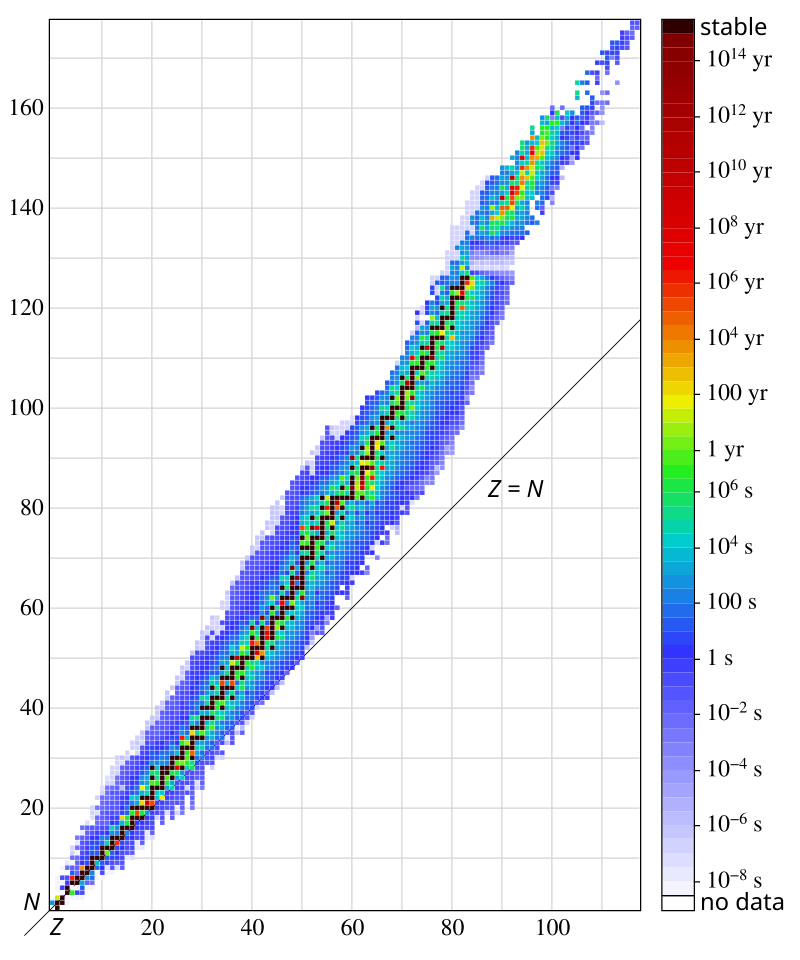
\includegraphics[width = 0.75\textwidth]{segre-chart.png}
  \caption{Tavola di Segré.}
  \label{segre-chart}
\end{figure}
\begin{figure}
  \centering
  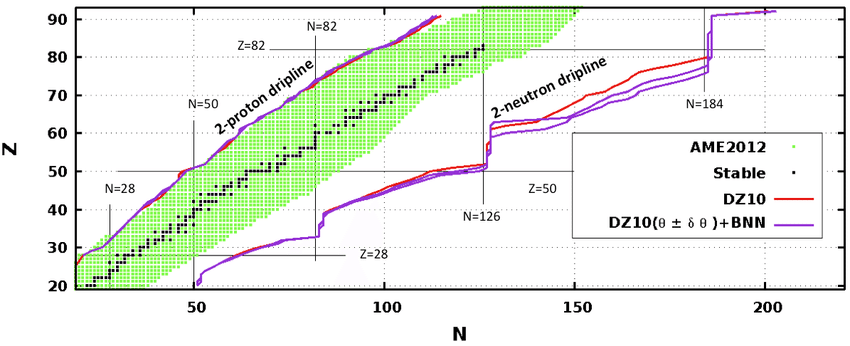
\includegraphics[width = 0.55\textwidth]{drip-lines.png}
  \caption{Nuclear driplines.}
  \label{drip-lines}
\end{figure}

\section{Evidenze sperimentali}

Le prime evidenze sperimentali dell'esistenza del nucleo atomico si devono al gruppo di ricerca di Rutherford, Geiger e Marsden: prima di loro, Thomson era riuscito ad estrarre delle cariche negative dall'atomo, identificando l'elettrone, ed aveva di conseguenza formulato la sua teoria della struttura atomica come sfera carica positivamente in cui sono immersi gli elettroni ($ \virgolette{plum pudding} $ model).\\
Con i loro esperimenti, Rutherford et al. dimostrarono invece che le cariche positive erano concentrate in una regione piccola al centro dell'atomo.

\subsection{Scattering di Rutherford}

L'esperimento condotto da Rutherford et al. consiste nell'irradiare una lamina sottile di oro con un fascio collimato di particelle $ \alpha $ (nuclei di $ \ch{^{4} He} $). Rutherford non aveva a disposizione acceleratori, e usò particelle $\alpha$ provenienti dai decadimenti radioattivi, con energie di pochi \mev, e dunque influenzate solo dall'interazione coulombiana. A livello puramente cinematico (ignorando la natura dell'interazione tra beam e target), essendo la velocità delle particelle $ \alpha $ $ v_0 \sim 0.1c $, è possibile trattare il problema come un urto elastico non-relativistico (conservazione della quantità di moto e dell'energia):
\begin{equation}
	\begin{cases}
	  m_{\alpha} \ve{v}_0 = m_{\alpha} \ve{v}_f + m_t \ve{v}_t \\
	  m_{\alpha} v_0^2 = m_{\alpha} v_f^2 + m_t v_t^2 \\
	\end{cases}
	\label{eq:2}
\end{equation}
Combinando le due equazioni e definendo $ \theta $ l'angolo tra $ \ve{v}_f $ e $ \ve{v}_t $ (velocità del target):
\begin{equation}
	\cos \theta = \frac{1}{2} \frac{v_t}{v_f} \left(1 - \frac{m_t}{m_{\alpha}}\right)
	\label{eq:3}
\end{equation}
Si possono distinguere due principali casi:
\begin{enumerate}
	\item $ m_t = m_e \ll m_{\alpha} $: $ \cos \theta > 0 $: la particella colpisce l'elettrone, e si parla di forward scattering, poiché non sono possibili grossi valori di $ \theta $ (deflessione) e la particella viene trasmessa attraverso il materiale;
	\item $ m_t = m_{Au} \gg m_{\alpha} $: $ \cos \theta < 0 $: urto tra oggetti massicci, dunque diventano possibili anche angoli di deviazione della traiettoria della particella $\alpha$ prossimi $ \pi $, e il rinculo del nucleo.
\end{enumerate}
Il modello di Thomson rientra nella prima casistica, poiché in tal caso all'interno dell'atomo lo scattering può avvenire solo con gli elettroni, che hanno $ m_e = 0.511 \mev/c^2 \ll m_{\alpha} = 4 \gev/c^2 \approx 4m_p , \frac{m_e}{m_{\alpha}} \approx 10^{-4} $. Questo implica che la massima quantità di moto trasferita al bersaglio elettronico è $\approx 10^{-4} p_i$, ovvero un piccolo cambiamento nella quantità di moto della particella $\alpha$.\\
Ciò che Rutherford et al. osservarono, però, è che occasionalmente delle particelle $ \alpha $ vengono riflesse dalla lamina d'oro: questo risultato è incompatibile con lo scattering con elettroni o con una carica positiva diffusa, dunque fu confermato che la carica positiva nell'atomo è concentrata in un unico punto massivo, il nucleo atomico. Infatti, $\frac{m_{Au-197}}{m_{\alpha}}\approx 50$, dove $m_{Au-197}=197 \gev/c^2$, ovvero il target è molto più massivo del proiettile. Questo implica che il nucleo può sottrarre fino al doppio del momento incidente, e la particella $\alpha$ può tornare indietro con una quantità di moto uguale e opposta a quella iniziale.

\subsubsection{Cross-section di Rutherford}

Nella trattazione cinematica è stata ignorata l'interazione tra particelle $ \alpha $ e nucleo atomico, che è ciò che effettivamente determina lo scattering: essa può essere modellata, in forma approssimativa (in particolare per parametro d'urto compreso tra il raggio nucleare e l'orbita elettronica più interna), dal potenziale coulombiano. Si assumono particelle puntiformi, poiché $\alpha$ non può penetrare nel nucleo. Dette $ Z $ il numero atomico dell'atomo target e $ Z' $ quello degli atomi del beam (nel caso specifico dello scattering di Rutherford $ Z = Z_{\ch{Au}} = 79 $ e $ Z' = Z_{\ch{He}} = 4 $), il potenziale d'interazione è:
\begin{equation}
	V(\ve{r}) = \frac{ZZ' e^2}{r}
	\label{eq:4}
\end{equation}
Dalla meccanica classica è possibile legare il parametro d'urto $ b $ all'angolo di scattering $ \theta $:
\begin{equation}
	b = \frac{ZZ' e^2}{2 E_0} \cot \frac{\theta}{2}
	\label{eq:5}
\end{equation}
dove $ E_0 $ è l'energia della particella incidente.\\
È possibile stimare quanto vicino al nucleo atomico si possono spingere le particelle $ \alpha $ tramite la distanza di closest approach $ a $, definita dalla condizione $ V(a) = E_0 $ ed esprimibile anche in funzione di $ b $ e $ \theta $ tramite $ \tan \frac{\theta}{2} = \frac{a}{2b} $: le particelle $ \alpha $ usate da Rutherford avevano $ E_{\alpha} \approx 5\mev $, dunque fu in grado di sondare il nucleo atomico poiché $ a \approx 45\fm $.\\
Per calcolare la cross-section dello scattering di Rutherford, si consideri un fascio incidente monoenergetico con energia $ E_0 $ e $ N_0 $ particelle incidenti per unità di area e di tempo: facendo variare il parametro d'urto tra $ b $ e $ b + db $, dunque variando l'angolo di scattering tra $ \theta $ e $ \theta - d \theta $, si avranno $ 2\pi N_0 b \,db $ particelle incidenti per unità di tempo (data la sezione d'urto $ \Delta\sigma = 2\pi b \,db $, Fig. \ref{rutherford}).
\begin{figure}
	\centering
	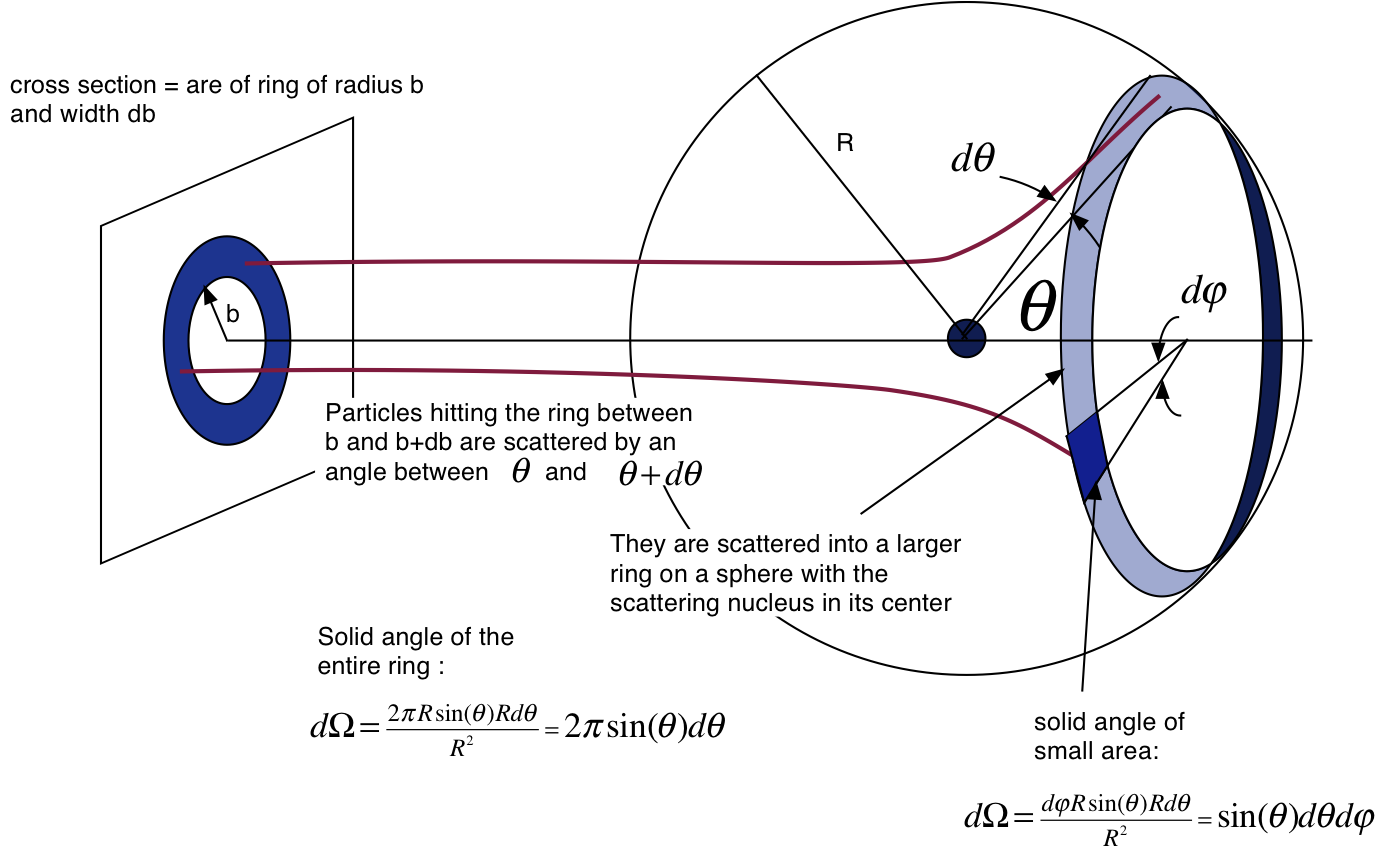
\includegraphics[width=0.95\textwidth]{rutherford.png}
	\caption{Sezione d'urto dello scattering di Rutherford.}
	\label{rutherford}
\end{figure}

Va notato che è possibile ignorare il fatto che la lamina target ha un numero elevato di atomi target e che ogni particella nel beam incidente ha un diverso parametro d'urto relativo a ciascuno di essi, poiché la lastra è considerata così sottile da rendere improbabili collisioni multiple della stessa particella incidente; inoltre, dal modello atomico di Rutherford ricaviamo che i nuclei atomici si trovano a distanze grandi rispetto alle loro dimensioni, rendendo significative solo le traiettorie con parametro d'urto vicino al nucleo atomico.\\
Nel caso di un potenziale d'interazione generico, $ \Delta\sigma $ può avere anche dipendenza azimuthale:
\begin{equation}
	\Delta\sigma(\theta,\phi) = b \,db\,d\phi = - \frac{d\sigma}{d\Omega} (\theta,\phi) \,d\Omega= - \frac{d\sigma}{d\Omega} (\theta,\phi) \sin \theta \,d\theta\,d\phi
	\label{eq:6}
\end{equation}
dov'è stata utilizzata la differential cross-section $ \frac{d\sigma}{d\Omega} $ e dove si è tenuto conto che un aumento di $ b $ porta ad una diminuzione di $ \theta $ tramite il segno negativo.\\
Essendo il potenziale coulombiano un potenziale centrale a simmetria sferica, è possibile semplificare il calcolo grazie alla simmetria azimuthale, ottenendo:
\begin{equation}
	\frac{d\sigma}{d\Omega} (\theta) = - \frac{b}{\sin \theta} \frac{db}{d\theta}
	\label{eq:7}
\end{equation}
Lo scattering di Rutherford può essere quindi completamente caratterizzato utilizzando l'Eq. \ref{eq:5}:
\begin{equation}
	\frac{d\sigma}{d\Omega} (\theta) = \left( \frac{ZZ' e^2}{4 E_0} \right)^2 \frac{1}{\sin^4 \frac{\theta}{2}}
	\label{eq:8}
\end{equation}
È anche possibile definire la sezione d'urto totale $ \sigma_{\text{tot}} $ come:
\begin{equation}
	\sigma_{\text{tot}} = \int_{\Omega} \frac{d\sigma}{d\Omega} (\theta,\phi) \,d\Omega
	\label{eq:9}
\end{equation}
Essa rappresenta una sorta di area di scattering effettiva che la sorgente del potenziale determina a tutti i possibili valori del parametro d'urto.\\
Nel caso dello scattering di Rutherford:
\begin{equation}
	\begin{split}
		\sigma_{\text{tot}} &= \int_0^{2\pi} \int_0^{\pi} \frac{d\sigma}{d\Omega} (\theta,\phi) \sin \theta \,d\theta\,d\phi = 2\pi \int_0^{\pi} \frac{d\sigma}{d\Omega} (\theta) \sin \theta \,d\theta \\
				    &= 8\pi \left( \frac{ZZ' e^2}{4 E_0} \right)^2 \int_0^1 \frac{1}{\sin^3 \frac{\theta}{2}} d\left( \sin \frac{\theta}{2} \right) \longrightarrow \infty
	\end{split}
	\label{eq:10}
\end{equation}
Questo risultato divergente è coerente con l'interpretazione data della sezione d'urto totale: il potenziale coulombiano è associato all'interazione elettromagnetica, la quale ha un range infinito, dunque anche l'area efficace di scattering sarà infita.\\
In maniera realistica, però, si può considerare che dopo un determinato valore di cutoff $ b_0 $ lo scattering non abbia più effetti osservabili sulla particella incidente, dunque la sezione d'urto totale osservabile si ottiene integrando la differential cross-section tra $ 0 $ e $ \theta_0 < \pi$, ottenendo dunque un valore finito.\\
La formula di Rutherford \ref{eq:8} cessa di essere valida quando $ E_0 $ diventa troppo alta, in particolare quando la particella $ \alpha $ riesce a penetrare nel nucleo, poiché a quel punto subentrano l'interazione nucleare fin'ora ignorata: studiando sperimentalmente a quale energia (a differenti angoli di scattering) si iniziano a manifestare le deviazioni dalla cross-section di Rutherford, è possibile stimare il raggio nucleare tramite la distanza di closest approach $ a $, trovando il fit sperimentale $ R = R_0 A^{1/3} $ con $ R_0 = 1.4\fm $.

\subsection{Scattering elettronico}

Data la dualità onda-particella che risulta da una descrizione quanto-meccanica della materia, la sezione d'urto da scattering non sarà determinata soltanto dall'interazione coulombiana ma anche da effetti diffrattivi, evidenziati dal pattern di diffrazione in Fig. \ref{diffraction}: l'analogo ottico è la diffrazione da disco opaco, poiché il nucleo atomico assorbe nucleoni, con la dovuta differenza che la superficie del nucleo ha una determinata diffusività, la quale determina dei minimi non-nulli nello spettro di diffrazione.
\begin{figure}
	\centering
	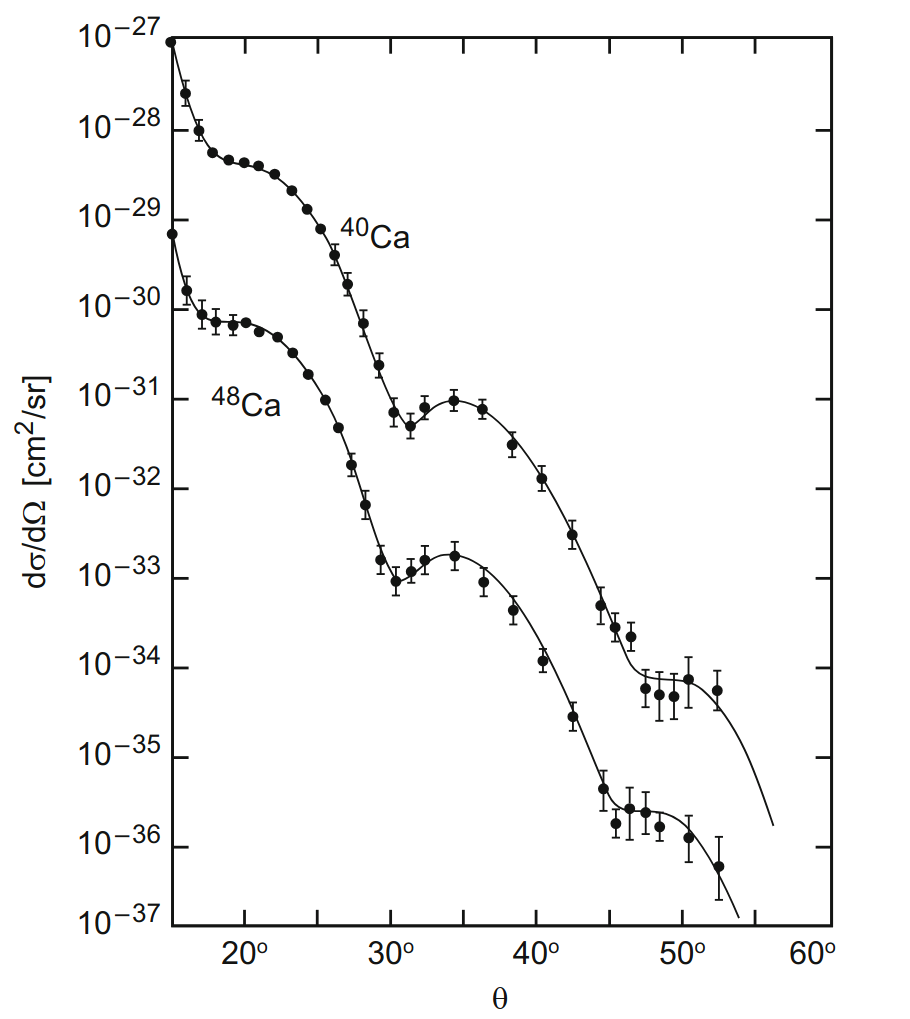
\includegraphics[width=0.95\textwidth]{diffraction.png}
	\caption{Sezione d'urto dello scattering elettronico.}
	\label{diffraction}
\end{figure}\\
Per evitare che all'interazione coulombiana si sovrapponga anche quella tra nucleoni, per studiare la struttura del nucleo atomico le sonde migliori sono gli elettroni: poiché per sondare una scala di lunghezze $ \Delta x $ è necessaria una lunghezza d'onda $ \lambda \sim \Delta x $, dalla relazione di de Broglie si ha che la quantità di moto degli elettroni incidenti deve essere $ p \sim h / \Delta x $. La struttura del nucleo atomico risulta visibile su scale di $ 1\fm $, dunque sono necessari elettroni con momento lineare $ p \approx 200 \mev/c $; nel caso si voglia studiare la struttura interna dei nucleoni, la stima aumenta di almeno un ordine di grandezza.\\
Va ricordato che gli elettroni, in quanto particelle cariche, quando percorrono una traiettoria curva irraggiano, dunque per questo tipo di scattering sono necessari accelleratori lineari.
Ricordando che $ E^2 = p^2 c^2 + m_0^2 c^4 $ ed $ E = K + m_0 c^2 $, considerando che $ m_e = 0.511 \mev/c^2 $, si vede che gli elettroni utilizzati per sondare il nucleo atomico sono in regime ultra-relativistico, dunque nel calcolo della cross-section sono da tenere in conto effetti relativistici legati allo spin ed il nuclear recoil (ovverosia il rinculo subito dal nucleo atomico a seguito dello scattering): trascurando quest'ultimo, si può applicare una correzione alla cross-section di Rutherford, detta cross-section di Mott:
\begin{equation}
	\left(\frac{d\sigma}{d\Omega}\right)_{\text{Mott}} = \left(\frac{d\sigma}{d\Omega}\right)_{\text{Ruth}} \left(1 - \beta^2 \sin^2 \frac{\theta}{2}\right)
	\label{eq:11}
\end{equation}
Queste sezioni d'urto, però, considerano scattering tra oggetti puntiformi, ma mentre un elettrone può effettivamente essere considerato tale, lo stesso non si può dire per il nucleo atomico, il quale avrà una certa distribuzione di carica $ \rho(\ve{r}) $ estesa nello spazio (essa coincide con la distribuzione di massa solo per nuclidi stabili); per considerare anche questo fatto, nel calcolo della cross-section si applica un'ulteriore correzione:
\begin{equation}
	\frac{d\sigma}{d\Omega} = \left(\frac{d\sigma}{d\Omega}\right)_{\text{Mott}} \abs{F(q)}^2
	\label{eq:12}
\end{equation}
dove $ \abs{F(q)}^2 $ è detto form factor e $ \ve{q} \defeq \frac{1}{\hbar} \abs{\ve{p}' - \ve{p}} $, con $ \ve{p} $ e $ \ve{p}' $ momento iniziale e finale dell'elettrone, esprime la variazione di quantità di moto dell'elettrone.\\
Dato che si sta considerando uno scattering elastico, si ha $ p = p' $ e dunque $ q = \frac{1}{\hbar} 2p \sin \frac{\theta}{2} $, con $ \theta $ angolo di scattering.\\
Nel caso dell'approssimazione di Born (elettroni come onde piane $ \psi(\ve{r}) = \frac{1}{\sqrt{V}} e^{i \ve{p}\cdot\ve{x} / \hbar} $) e trascurando il nuclear recoil, il form factor è la trasformata di Fourier della distribuzione di carica $ \rho(\ve{r}) $:
\begin{equation}
	F(q) = \int_{r \le R} e^{i \ve{p}\cdot\ve{r} / \hbar} \rho(\ve{r}) d^3\ve{r}
	\label{eq:13}
\end{equation}
con $ R $ raggio nucleare ed opportuna normalizzazione $ F(0) = 1 $.\\
In questa approssimazione, quindi, una misura della cross-section di scattering elettronico può dare informazioni sulla distribuzione di carica nel nucleo atomico; inoltre, è possibile dare una stima del raggio nucleare dallo studio dello spettro di diffrazione evidenziato dalla cross-section, poiché il primo minimo di diffrazione soddisfa la relazione $ \frac{q}{\hbar} \approx \frac{4.5}{R} $; se invece si considerano due isotopi, dal fatto che la separazione angolare tra due minimi è $ \Delta\theta = \frac{\hbar}{p R} $ si evince che all'aumentare del numero di massa aumenta anche il raggio nucleare (vedere Fig. \ref{diffraction}): ciò in generale è valido solo per nuclidi nella cosiddetta $ \virgolette{valle di stabilità} $, poiché per essi la distribuzione di neutroni segue quella di protoni, ovvero le distribuzioni ci carica e massa vanno a coincidere, dunque un nuclide con più nucleoni avrà un raggio nucleare maggiore; la difficoltà principale nella misura della distribuzione di nucleoni sta nel fatto che i neutroni sono trasparenti agli esperimenti di scattering, poiché non interagiscono né tramite interazione elettromagnetica né tramite interazione nucleare forte.

\subsubsection{Distribuzione di carica nucleare}

Compiendo esperimenti di scattering elettronico e raccogliendo dati relativi a vari nuclei atomici, si è giunti alla conclusione che i nuclidi non sono sfere con un confine ben delineato, ma al loro interno la densità di carica si mantiene approssimativamente costante, mentre verso la superficie essa si riduce su un intervallo radiale relativamente ampio; la distribuzione di carica nucleare può dunque essere approssimata da una distribuzione di Fermi:
\begin{equation}
	\rho(\ve{r}) = \frac{\rho_0}{1 + e^{(r - c) / a}}
	\label{eq:14}
\end{equation}
dove i parametri empirici valgono (per nuclei pesanti) $ c = 1.07\fm \cdot A^{1/3} $ e $ a = 0.54\fm $: $ c $ è il raggio nucleare a mezza altezza della distribuzione di carica, mentre $ a $ è la diffusività (ciò che rende la distribuzione smooth piuttosto che sharp).\\
Una volta nota la distribuzione di carica, è possibile calcolare il raggio quadratico medio: per nuclei medi e pesanti, si ha $ \sqrt{\langle r^2 \rangle} = 0.94\fm \cdot A^{1/3} $. Se si approssima il nucleo come una sfera uniformemente carica, il suo raggio, definito come raggio nucleare, è dato da $ R^2 = \frac{5}{3} \langle r^2 \rangle $, ovvero:
\begin{equation}
	R = 1.21\fm \cdot A^{1/3}
	\label{eq:14-bis}
\end{equation}
che è la definizione più diffusa di raggio nucleare.\\
È anche possibile definire una skin depth (o surface thickness) $ t $ come lo spessore del guscio sferico in cui la densità di carica diminuisce dal $ 90\% $ al $ 10\% $ del suo valore massimo: per nuclei pesanti, si trova $ t = 2a\ln9 \approx 4.4 a $.\\
Come si può vedere in Fig. \ref{charge-distr}, la densità di carica centrale $ \rho_0 $ diminuisce leggermente all'aumentare del numero di massa; se però viene considerata la presenza di neutroni e si moltiplica per un fattore $ A / Z $, si trova un valore quasi identico per tutti i nuclidi (questo è coerente con $ R \sim A^{1/3} $, poiché così $ \rho_0 \sim A / \text{Vol} $ rimane costante): questo corrisponde alla densità che teoricamente avrebbe della materia nucleare infinitamente estesa, pari a $ \rho_n \approx 0.17 \,\text{nucleoni} / \text{fm}^3 $, che corrisponde a $ c = 1.12\fm \cdot A^{1/3} $.
\begin{figure}[!ht]
	\centering
	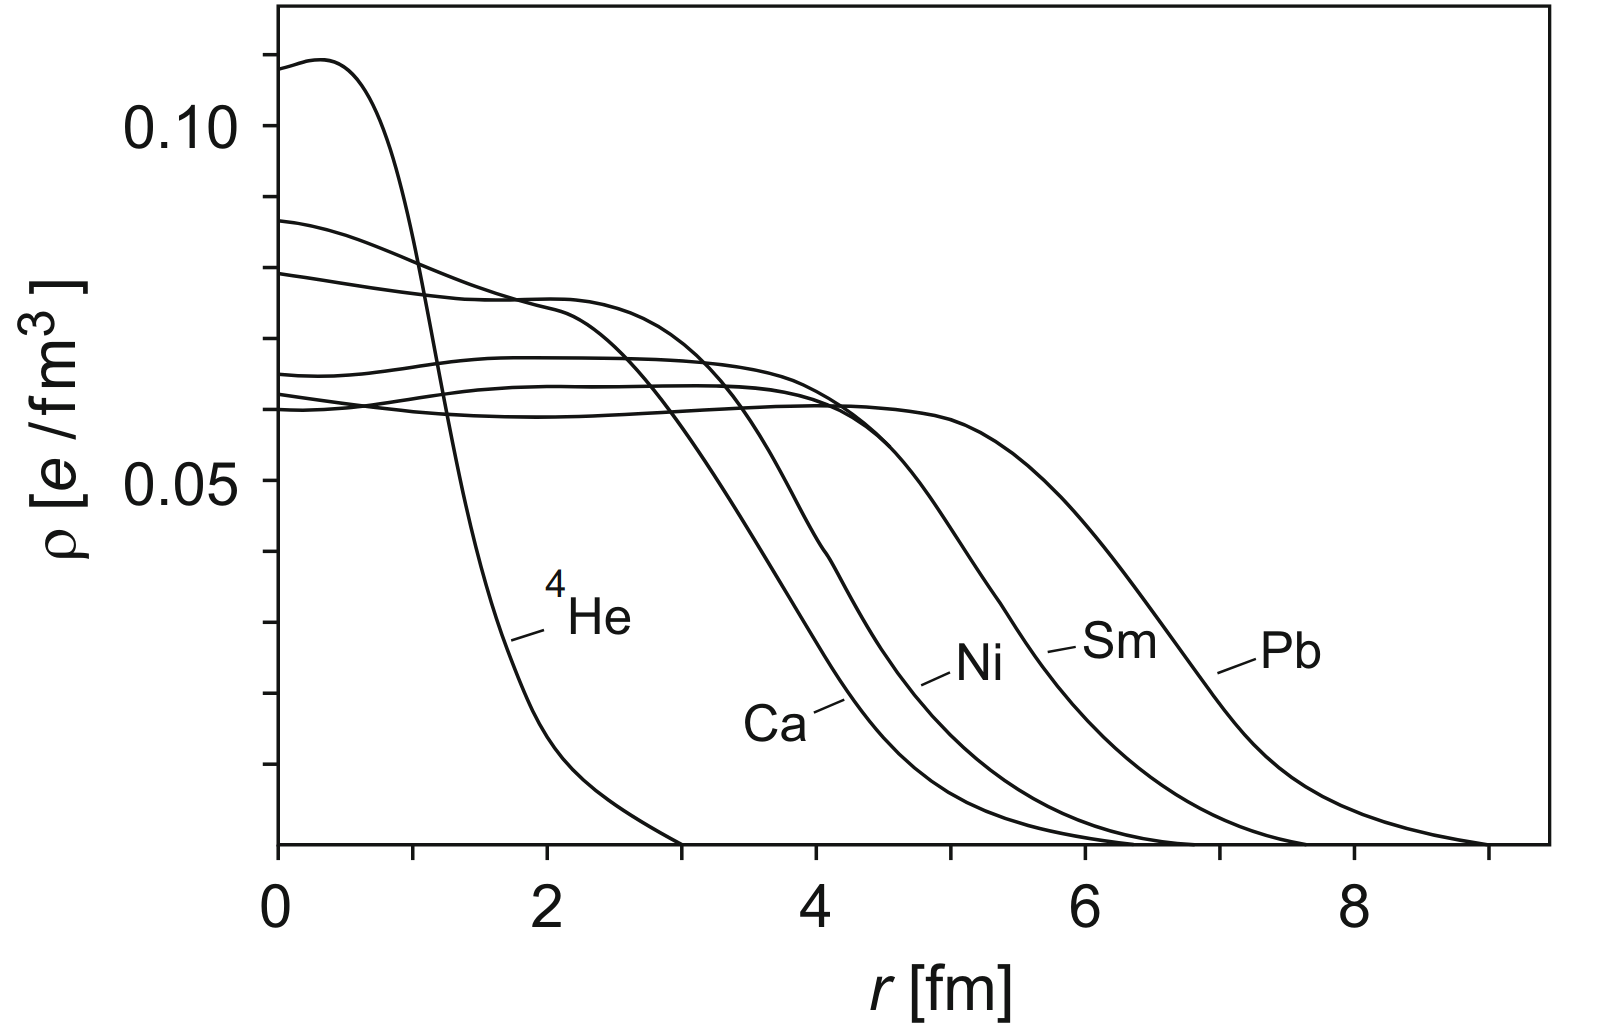
\includegraphics[width=0.95\textwidth]{charge-distribution.png}
	\caption{Distribuzione di carica in vari nuclidi.}
	\label{charge-distr}
\end{figure}

Sperimentalmente si trova che alcuni nuclidi (ad esempio i lantanidi) non hanno una forma sferica ma assumono deformazioni ellissoidali: queste forme non possono essere studiate con scattering elettronico, poiché esso evidenzia soltanto una superficie molto diffusa.\\
Va infine notato che nuclidi leggeri come $ \ch{^{6,7}Li} $, $ \ch{^{9}Be} $ e soprattutto $ \ch{^{4}He} $ costituiscono dei casi speciali: essi non presentano una densità di carica centrale costante, ma il suo andamento è approssimativamente gaussiano.

\subsubsection{Nuclidi instabili}

Quanto riportato fin'ora vale solo per nuclidi nella valle di stabilità (vedere Fig. \ref{segre-chart}), ovverosia l'insieme di nuclei stabili che non decadono radioattivamente (tipicamente per decadimento $ \beta $), i quali sono osservati in abbondanza sulla Terra.\\
Se, partendo dalla valle di stabilità, si percorre una catena isotopica, i nuclidi diventano via via più neutron-rich, fino a quando non si raggiungono le driplines, oltre le quali i nuclei non sono più sistemi legati a causa dell'interazione nucleare forte.\\
Lo spostamento verso nuclidi esotici neutron-rich causa un mutamento drastico rispetto ai loro isotopi stabili: in un lavoro pionieristico del 1985 di Tanihata et al., fu misurata la cross-section d'interazione tra nuclei di $ \ch{^{11}Li} $ (isotopo instabile) e dei nuclidi stabili target, la quale può essere teoricamente calcolata dal modello di Glauber per lo scattering relativistico di nuclidi (traiettorie iniziali e finali rettilinee) come $ \sigma_I \sim \pi \left( R_p^2 + R_t^2 \right) $, dove $ R_p $ è il raggio del nucleo proiettile ed $ R_t $ quello del nucleo target; dai dati fu possibile ricavare il raggio nucleare del $ \ch{^{11}Li} $, il quale dovrebbe essere dell'ordine di $ \sim 2.4\fm $, trovando un valore cinque volte maggiore (comparabile con quello del $ \ch{^{208}Pb} $): questa fu la prima verifica sperimentale dell'esistenza di sistemi ad alone, nuclidi con un corpo centrale sferico circondati da uno o due neutroni o protoni (si parla di neutron skin o proton skin), i quali vanno a formare un halo attorno al nucleo aumentandone considerevolmente le dimensioni osservate.\\
Condurre esperimenti di scattering elettronico su nuclei instabili è estremamente difficile, poiché pochi di essi hanno delle vite medie abbastanza lunghe, dunque non è possibile predisporre un target composto del materiale da studiare: in alcuni laboratori si è riusciti a costruire delle trappole con le quali i nuclidi instabili sono accellerati e confinati, così da poter essere bombardati da fasci elettronici.

\paragraph{Luminosità}

Nello studio dei rilevatori di scattering un importante parametro è la luminosità:
\begin{equation}
	\mathcal{L} = N_b N_t
	\label{eq:15}
\end{equation}
dove $ N_b $ è il numero di particelle incidenti per unità di tempo e $ N_t $ il numero di nuclidi target per unità d'area.\\
Questo parametro è legato all'efficienza del rilevatore, misurata dal numero di eventi rilevati nell'unità di tempo $ \dot{N} $:
\begin{equation}
	\dot{N} (E, \theta) = \mathcal{L}\, \frac{d\sigma}{d\Omega} (E,\theta) \,\Delta\Omega
	\label{eq:16}
\end{equation}
Nel caso dello scattering elettronico, la cross-section è molto piccola, dunque sono necessari collisori dall'elevata luminosità (tecnicamente difficile): si va da $ \mathcal{L}_{\text{min}} \sim 10^{26} \,\text{cm}^{-2} \,\text{s}^{-1} $ per sondare nuclidi con $ Z \sim 80 $ a $ \mathcal{L}_{\text{min}} \sim 10^{31} \,\text{cm}^{-2}\,\text{s}^{-1} $ per $ Z \sim 10 $.\\
Inoltre, la luminosità varia anche in base al target considerato: per nuclidi stabili si raggiungono luminosità per scattering elettronico di $ 10^{33} \,\text{cm}^{-2}\,\text{s}^{-1} $ (es: STABLE), mentre su nuclidi instabili si arriva a $ 10^{27} \,\text{cm}^{-2}\,\text{s}^{-1} $ (es: SCRIT).

\section{Proprietà dei nuclidi}

\subsection{Masse nucleari}

Preso un atomo di una specie chimica $ ^A_Z \text{X}_N $, se si sommano le masse degli $ N $ neutroni, dei $ Z $ protoni e dei $ Z $ elettroni, si trova una massa minore di quella misurata per l'atomo: questo avviene poiché, essendo l'atomo uno stato legato, parte della massa dei suoi costituenti viene convertita in energia di legame (positiva, poiché stato legato), ovvero:
\begin{equation}
	M_{\text{atom}} = N m_n + Z \left( m_p + m_e \right) - \frac{1}{c^2} \left( B_{\text{atom}} + B_{\text{nucleus}} \right)
	\label{eq:1.17}
\end{equation}
dove si è distinto tra binding energy atomica e nucleare: queste ultime sono conosciute con incertezze maggiori, dato che $ (\delta m / m)_{\text{atom}} \sim 10^{-10} $ e $ (\delta m / m)_{\text{nucleus}} \sim 10^{-7} $.\\
Si trova quindi che la binding energy di un nuclide può essere espressa come:
\begin{equation}
	B(A,Z) = \left[ Z m({\ch{^{1}H}}) + N m_n - M(A,Z) \right] c^2
	\label{eq:1.18}
\end{equation}
dove si sono usate le masse atomiche, poiché misurate con più precisione (si ricordi la conversione $ 1u \approx 931.494\mev/c^2 $).\\
La misura delle masse atomiche è importante poiché permette di fare misure indirette sulle masse nucleari, e dunque studiare l'abbondanza isotopica di un elemento, e di stimare le binding energies, le quali sono legate alla natura della forza nucleare.\\
Ci sono varie tecniche per misurare le masse atomiche: spettrometri di massa, cinematica delle reazioni (solitamente quando i primi non si possono utilizzare), trappole (ad oggi gli strumenti più precisi) ed anelli di accumulazione (storage rings).

\subsubsection{Spettrometri di massa}

Uno spettrometro di massa permette di misurare le masse di ioni di un determinato elemento.
\begin{figure}[!b]
	\centering
	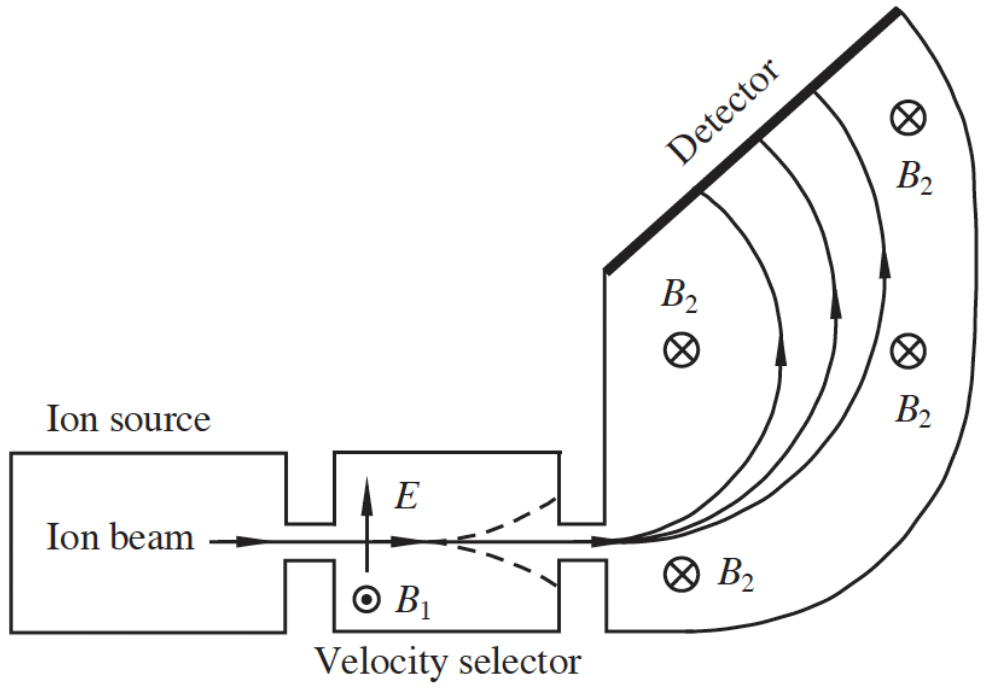
\includegraphics[width=0.75\textwidth]{spectrometer.png}
	\caption{Schematizzazione di uno spettrometro di massa.}
	\label{spettr}
\end{figure}

Schematicamente (Fig. \ref{spettr}), esso è costituito da:
\begin{itemize}
	\item una sorgente di ioni;
	\item un selettore di velocità;
	\item uno spettrometro magnetico;
	\item un focal plane detector.
\end{itemize}
La sorgente di ioni ionizza gli atomi da studiare, li accellera e li collima in un fascio; questo fascio viene diretto in un selettore di velocità: questo è solitamente un filtro di Wien, composto da un campo elettrico e un campo magnetico incrociati che determinano traiettorie rettilinee solo se $ \ve{F}_E + \ve{F}_B = \ve{0} $, ovvero, assumendo un fascio già collimato nella direzione desiderata, se $ v = E / B $.\\
L'elemento ottico di questo setup è lo spettrometro magnetico: in esso le traiettorie degli ioni curvano in base al loro momento e alla loro carica, dato che il raggio di girazione è $ r = \frac{vm}{qB} $: di conseguenza, sperimentalmente vanno misurati sia il raggio di girazione che la carica per poter determinare la massa dello ione, e ciò è proprio quello che fa il focal plane detector.\\
Va notato che, in generale, le misure assolute di massa non permettono una grande precisione, perciò si preferisce effettuare misurazioni rispetto a ioni di cui già di conosce bene la massa: in particolare, le precisioni maggiori si raggiungono sui mass ratios tra ioni di egual carica, poiché in tal caso $ m_1 / m_2 = r_1 / r_2 $. Il campione di riferimento solitamente utilizzato è il carbonio, poiché dati i suoi numerosi composti permette di effettuare misure su un vasto range di ioni.

\paragraph{Abbondanze isotopiche}

Tendenzialmente, un elemento avrà più di un isotopo stabile (if any at all), dunque con una spettrografia di massa risulterà una distribuzione di massa con picchi di abbondanza relativa corrispondenti agli isotopi stabili: ciò permette di misurarne le masse $ m_i $ e l'abbondanza percentuale nel campione $ w_i $, così da poter stimare la massa atomica dell'elemento come media ponderata $ m = \sum_{i} w_i m_i $.\\
In generale, le abbondanze isotopiche sono diverse nell'Universo rispetto alla Terra, ed anche sulla Terra possono avere forti fluttuazioni tra una zona geografica e l'altra; ad esempio, si considerino due campioni di $ \ch{Xe} $, uno prelevato da una roccia metamorfica vecchia di $ 2.7 \text{Gy} $ ed uno dall'atmosfera: le relative analisi spettrografiche (riportate in Fig. \ref{iso-distr}) mostrano delle diverse abbondanze isotopiche nei due campioni, dovute alla presenza nella roccia metamorfica di prodotti della fissione nucleare spontanea dell'uranio.
\begin{figure}[!b]
	\centering
	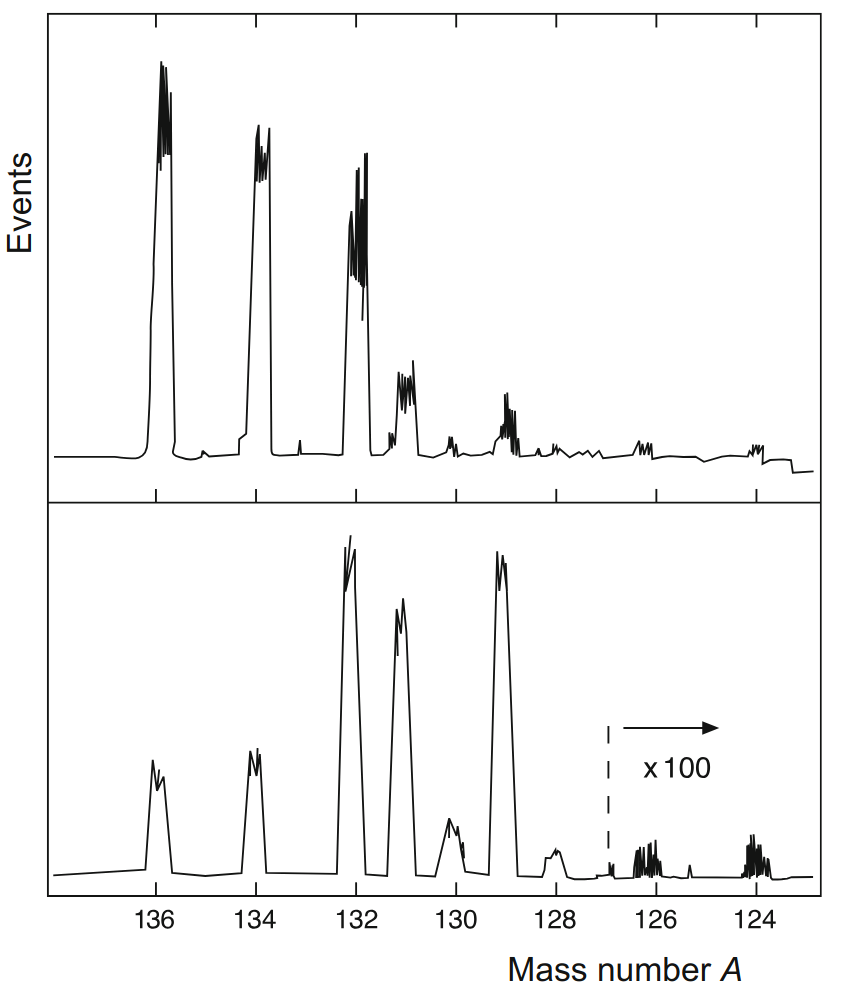
\includegraphics[width=0.55\textwidth]{isotop-distr.png}
	\caption{Distribuzioni isotopiche di due campioni di $ \ch{Xe} $, il primo prelevato da una roccia metamorfica, il secondo dall'atmosfera.}
	\label{iso-distr}
\end{figure}

\begin{figure}[!ht]
	\centering
	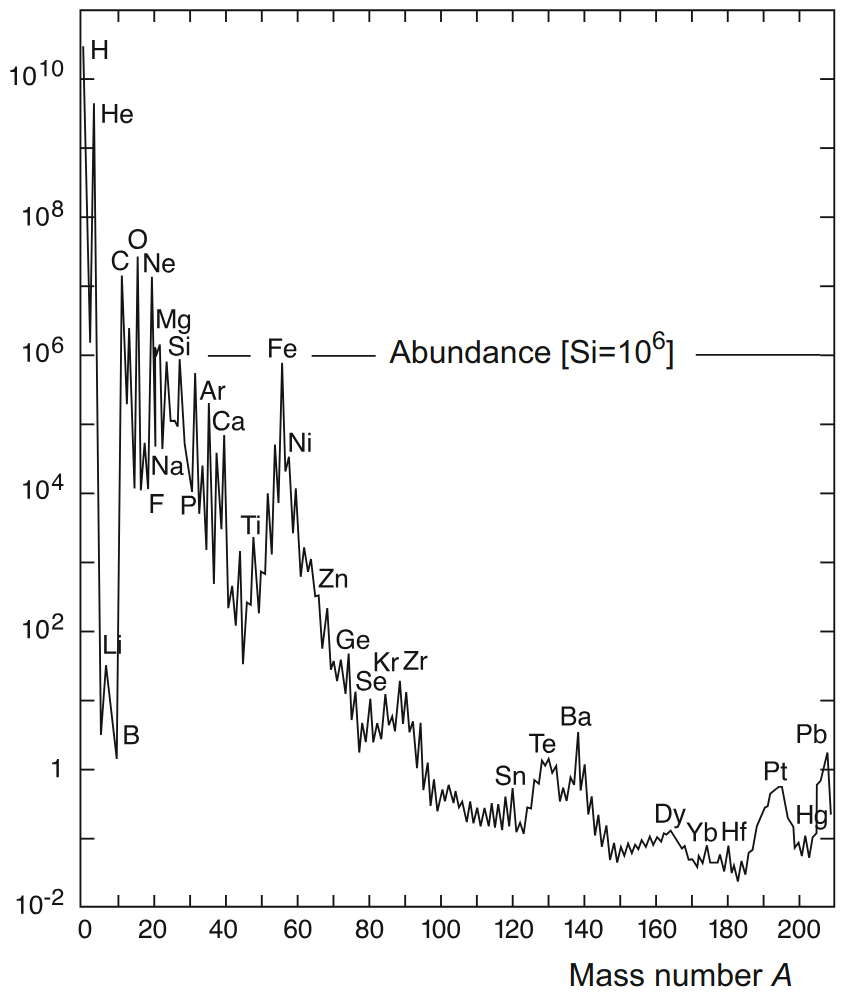
\includegraphics[width=0.75\textwidth]{isotop-distr-univ.png}
	\caption{Distribuzioni isotopiche dei principali elementi nel Sistema Solare, normalizzati all'abbondanza del $ \ch{Si} $: l'abbondanza del $ \ch{Li} $ è uno dei problemi nella ricostruzione dell'origine dell'Universo.}
	\label{iso-distr-univ}
\end{figure}
Lo studio delle abbondanze relative nell'Universo (Fig. \ref{iso-distr-univ}) permette di studiarne l'evoluzione: secondo gli attuali modelli, la sintesi di deuterio ed elio è avvenuta all'origine dell'Universo dalla fusione nucleare dell'idrogeno, mentre i nuclidi fino al $ \ch{^{56}Fe} $ vengono sintetizzati dalla fusione nucleare nei nuclei stellari; per quanto riguarda i nuclei pesanti, invece, la loro sintesi avviene nelle esplosioni di stelle molto massive.

\subsubsection{Cinematica delle reazioni}

Qualora il tempo di volo tra il generatore di ioni ed il piano focale fosse maggiore della vita media dello ione che si vuole studiare, al posto della spettroscopia di massa è possibile calcolare la massa dello ione studiandone le sue reazioni.\\
Si consideri una reazione del tipo:
\begin{equation}
	a + \text{X} \longrightarrow b
	\label{eq:1.19}
\end{equation}
dove $ a $ è la particella proiettile, $ \text{X} $ lo ione target e $ b $ rappresenta l'insieme di prodotti della reazione.\\
Assumendo uno scattering elastico, la conservazione dell'energia ci dà:
\begin{equation}
	m_a c^2 + T_a + m_{\text{X}} c^2 + T_{\text{X}} = m_b c^2 + T_b
	\label{eq:1.20}
\end{equation}
È possibile definire il cosiddetto Q-value della reazione:
\begin{equation}
	Q \defeq T_{\text{final}} - T_{\text{initial}} = T_b - T_a - T_{\text{X}}
	\label{eq:1.21}
\end{equation}
così da poter calcolare la massa dell'isotopo $ \text{X} $ come:
\begin{equation}
	m_{\text{X}} = \frac{1}{c^2} Q + m_b - m_a
	\label{eq:1.22}
\end{equation}
Con questo metodo, è possibile raggiungere una precisione $ \delta m / m \sim 10^{-6} $.

\subsubsection{Trappole}

Le trappole sono dispositivi in grado di confinare ioni grazie a campi elettromagnetici finemente controllati. Esse vengono usate soprattutto quando la vita media dello ione radioattive non permette l'utilizzo né di spettrometri di massa (a causa del tempo di volo) né di reazioni cinematiche (per sezioni d'urto bassissime).\\
Il vantaggio delle trappole è che permettono lo studio prolungato anche di singoli radioisotopi in regimi energetici bassissimi, dunque con velocità pressoché nulle, limitatamente alle loro vite medie.\\
Sebbene le trappole abbiano incertezze relative bassissime ($ \delta m / m \sim 10^{-8} $ per nuclidi instabili e $ 10^{-11} $ per nuclidi stabili), in determinati si sceglie di usare gli anelli di accumulazione poiché, nonostante le incertezze leggermente più alte, permettono di raggiungere energie relativistiche, rendendo possibili misurazioni su isotopi con vite medie cortissime.

\paragraph{Trappola di Penning}

Una trappola costituita da 4 elettrodi pensata per isotopi prodotti con velocità basse (principalmente tecnica ISOL\footnote{Ioni incidono su una lastra di carbonato di uranio a $ 4000\cels$ così da poter effondere e diffondere attraverso la superficie con un'energia cinetica bassissima; sono possibili anche tecniche di accellerazione e post-accellerazione.}), i quali vengono confinati radialmente da un campo magnetico (per moto di ciclotrone) ed assialmente da un campo elettrostatico di quadrupolo.\\
Il moto all'interno della trappola è molto complicato, poiché somma di un moto di magnetone circolare attorno all'asse di $ \ve{B} $ con frequenza $ \omega_- $, un moto di ciclotrone spiraleggiante attorno alle linee di $ \ve{B} $ con frequenza $ \omega_+ $ ed un moto oscillatorio longitudinale determinato da $ \ve{E}_{\text{quad}} $ con frequenza $ \omega_z $. Si dimostra il seguente teorema d'invarianza:
\begin{equation}
	\omega_c^2 = \omega_+^2 + \omega_-^2 + \omega_z^2
	\label{eq:1.23}
\end{equation}
Ciò permette di misurare la massa dello ione, ricordando che la frequenza di ciclotrone è $ \omega_c = \frac{q B}{m} $.\\
Le misure effettuate sono sempre misurazioni relative di massa (solitamente con campione $ \ch{^{12}C} $), così da includere eventuali errori sistematici.

\subsubsection{Anelli di accumulazione}

Un anello di accumulazione è un accelleratore di particelle circolare in cui un fascio di ioni viene fatto circolare a velocità relativistica per un periodo prolungato di tempo.\\
Gli ioni vengono prodotti con velocità relativistiche (principalmente tecnica in flight\footnote{Nuclei radioattivi (es: $ \ch{^{238}U} $) vengono accellerati a diverse centinaia di MeV per nucleone e fatti scontrare su target di $ \ch{^{9}Be} $, frammentandosi in prodotti con velocità relativistiche, i quali vengono poi selezionati da strumenti ottici in base al rapporto $ m/q $.}) ed immessi nell'anello; la loro massa è determinata dal periodo di rivoluzione:
\begin{equation}
	\frac{\Delta T}{T} = \frac{1}{\gamma_t^2}\frac{\Delta (m/q)}{m/q} - \left( 1 - \frac{\gamma^2}{\gamma_t^2} \right) \frac{\Delta v}{v}
	\label{eq:1.24}
\end{equation}
Il secondo termine è una correzione dovuta alla transition energy (il valore per cui l'energia diventa indipendente dalla specie chimica nell'anello) e alla dispersione delle velocità, ed è eliminabile tramite tecniche ingegneristiche: in particolare, esistono anelli di accumulazione progettati col metodo di Schottky (cool fragments), per i quali $ \frac{\Delta v}{v} \rightarrow 0 $, e quelli a traiettorie isocrone (hot fragments, così da avere energia pari all'energia di transizione), per i quali $ \gamma_t \rightarrow \gamma $. Con questi anelli di accumulazione si raggiunge $ \delta m / m \sim 10^{-8} $.

\subsection{Binding energy}

Riprendendo l'Eq. \ref{eq:1.18}, si definisce la binding energy di un nuclide $ ^A_Z \text{X}_N $ come:
\begin{equation}
	B(A,Z) = \left[ Z m({\ch{^{1}H}}) + N m_n - M(A,Z) \right] c^2
	\label{eq:1.25}
\end{equation}
La binding energy è positiva nel caso di nuclidi legati, ovvero quelli che possono effettivamente esistere nel loro stato fondamentale (anche se con vite medie corte).\\
Come si può vedere in Fig. \ref{bind-en}, se si restringe l'analisi ai nuclidi stabili e long-lived, si nota che, a seguito di rapide variazioni per bassi $ A $, la binding energy per nucleone si stabilizza a circa $ 8\mev/\text{nucleone} $ per i pesanti (oltre il $ \ch{^{56}Fe} $): i nuclei più stabili sono $ \ch{^{62}_{28}Ni} $, $ \ch{^{58}_{26}Fe} $ e $ \ch{^{56}_{26}Fe} $.
\begin{figure}[!ht]
	\centering
	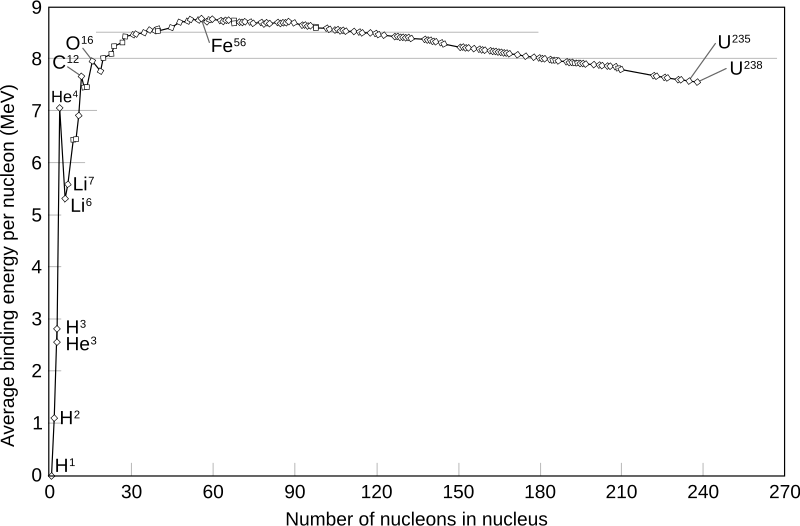
\includegraphics[width=0.75\textwidth]{bind-en.png}
	\caption{Binding energy table for stable and long-lived nuclei.}
	\label{bind-en}
\end{figure}

Sempre dal grafico in Fig. $ \ref{bind-en} $ è possibile fare alcune considerazioni:
\begin{enumerate}
	\item i nuclei pari-pari (numero pari di neutroni e di protoni) sono energeticamente favoriti rispetto a quelli pari-dispari, poiché più legati (es: $ \ch{^{4}He} $ è il nuclide leggero più legato), inoltre non ci sono nuclidi stabili per $ A = 5,8 $;
	\item il rapporto $ B/A \sim 8\mev $ costante per i nuclei pesanti evidenzia la natura a corto raggio dell'interazione forte, la quale viene saturata (un nucleone risente solo dei nucleoni vicini);
	\item il picco attorno ad $ A \sim 60 $ mostra come, tendendo all'equilibrio, i nuclidi leggeri guadagnano energia formando nuclei più pesanti tramite fusione nucleare (es: ambiente stellare), mentre i nuclidi pesanti perdono energia separandosi in nuclei leggeri tramite fissione nucleare.
\end{enumerate}
È necessario fare una precisazione: un nuclide può essere legato ma comunque instabile. Ad esempio, il $ \ch{^8 Be} $ ha $ B = 56.5\mev $, ma rispetto al decadimento $ \alpha $ si ha $ \ch{^8 Be} \rightarrow 2\alpha $, il quale ha una variazione d'energia $ B_{\text{decay}} = - 0.092\mev $: si evince che nel suo stato fondamentale il $ \ch{^8 Be} $ non esiste in uno stato legato, ma come risonanza di due particelle $ \alpha $, la quale sussiste per un certo periodo di tempo prima di decadere.\\
In generale, se esiste almeno una combinazione di neutroni e protoni non legata, allora il nuclide allo stato fondamentale non esiste in uno stato legato e decade; inoltre, di solito sono possibili varie modalità di decadimento, dette decay branches.

\subsubsection{Formula semi-empirica di Weizsäcker}

È possibile dare un'interpretazione fenomenologica della binding energy tramite un modello semplificato del nucleo atomico: il modello a goccia. Questo modello si basa sulle seguenti ipotesi:
\begin{enumerate}
	\item l'energia d'interazione tra due nucleoni è indipendente dal tipo e dal numero di nucleoni (non si distingue tra neutroni e protoni);
	\item l'interazione tra nucleoni è attrattiva a breve raggio per $ r < R_{\text{int}} $ e repulsiva a brevissimo raggio per $ r \ll R_{\text{int}} $;
	\item la binding energy del nucleo è proporzionale al numero di nucleoni (e dunque al volume del nucleo).
\end{enumerate}
Questo modello implica delle forze sature tra nucleoni, in cui ciascuno nucleone è legato solo ai nucleoni immediatamente vicini; definendo l'energia d'interazione tra due nucleoni $ \langle U \rangle $, ciò implica che la binding energy del nucleo non è data dalla somma di tutte le coppie di nucleoni, ma solo delle coppie vicine in un volume $ V_{\text{int}} < V_{\text{nucleo}} $. Ricordando che $ V_{\text{nucleo}} \sim A $, si ha:
\begin{equation}
	B_0 = \sum_{r < R_{\text{int}}} U = \frac{A(A-1)}{2}\langle U \rangle \frac{V_{\text{int}}}{V_{\text{nucleo}}} \sim b_0 A
	\label{eq:1.26}
\end{equation}
A questa stima cruda vanno aggiunti dei termini correttivi per effetti di cui il modello a goccia non tiene conto.\\
Innanzitutto, va considerato un termine di superficie, dovuto al fatto che i nucleoni sulla superficie del nucleo interagiscono con un minor numero di nucleoni, dunque sono meno legati; dato che il raggio atomico è $ R \sim A^{1/3} $, il termine di superficie va come $ B_{\text{sup}} \sim - b_1 A^{2/3} $.\\
Bisogna anche considerare la repulsione coulombiana tra protoni, la quale può essere approssimata col modello della sfera uniformemente carica (dai form factors, $ \rho $ è circa costante all'interno del nucleo):
\begin{equation}
	 U_e = \int_0^R V(r) \rho(r) 4\pi r^2 dr = \int_0^R \frac{Ze}{4\pi \epsilon_0 r} \left( \frac{r}{R} \right)^3 \frac{Ze}{\frac{4}{3}\pi R^3} 4\pi r^2 dr = \frac{3}{5} \frac{(Ze)^2}{4\pi \epsilon_0 R}
	\label{eq:1.27}
\end{equation}
Dunque va aggiunta una correzione $ B_{\text{Coulomb}} \sim - b_2 \frac{Z^2}{A^{1/3}} $.\\
Essendo il nucleo un sistema quantistico, è naturale che nella sua descrizioni siano inclusi gli effetti quantistici: in particolare, il calcolo dell'energia cinetica dei nucleoni può essere svolto prendendo come modello un gas di Fermi, il quale tiene conto della statistica dei fermioni e del principio di esclusione di Pauli (questo favorisce la formazione di nuclei con egual numero di protoni e neutroni); l'energia cinetica totale risulta essere:
\begin{equation}
	K_{\text{tot}} \approx 20 \mev \left( A + \frac{5}{9} \frac{(N - Z)^2}{A} \right)
	\label{eq:1.28}
\end{equation}
Il primo termine si aggiunge al termine di volume $ B_0 $, mentre il secondo termine determina un termine correttivo $ B_{\text{sym}} \sim - b_3 \frac{(N - Z)^2}{A} $.\\
Infine, lo studio delle masse nucleari mostra che i nuclei con un numero pari di protoni e/o neutroni sono più stabili: ciò viene interpretato come un accoppiamento a doppietti sia dei protoni che dei neutroni (in base ai loro spin e momento angolare, in modo da avere spin totale nullo). Empiricamente, ciò determina un fattore correttivo alla binding energy pari a:
\begin{equation}
	B_{\text{parity}} \sim - \delta A^{-1/2}, \qquad \delta =
	\begin{cases}
		+11.2\mev & \text{dispari-dispari} \\
		0\mev & \text{dispari-pari o pari-dispari} \\
		-11.2\mev & \text{pari-pari}
	\end{cases}
	\label{eq:1.29}
\end{equation}
Si è sostanzialmente ricavata la \textit{formula semi-empirica di Weizsäcker}:
\begin{equation}
	B(A,Z) = a_V A - a_S A^{2/3} - a_C \frac{Z^2}{A^{1/3}} - a_a \frac{(N - Z)^2}{A} - \delta A^{-1/2}
	\label{eq:1.30}
\end{equation}
dove $ \delta $ è definito in Eq. $ \ref{eq:1.29} $ e gli altri parametri fenomenologici si trovano essere $ a_V = 15.835\mev $, $ a_S = 18.33\mev $, $ a_C = 0.714\mev $ e $ a_a = 23.20\mev $.\\
Lungo le catene isotopiche ($ A = $ const.) $ B(Z) $ è una parabola: è possibile trovare $ Z_{\text{min}} $ analiticamente, ottenendo che per $ A $ grande è $ Z_{\text{min}} < \frac{A}{2} $, mentre per $ A $ piccolo $ Z_{\text{min}} \approx \frac{A}{2} $, e questa condizione dà il nuclide più stabile della catena isotopica considerata. Nel caso di catene con $ A $ pari, si ha una doppia parabola a causa del termina di pairing $ \delta $ (vedere Fig. \ref{iso-chain}).
\begin{figure}[!h]
	\centering
	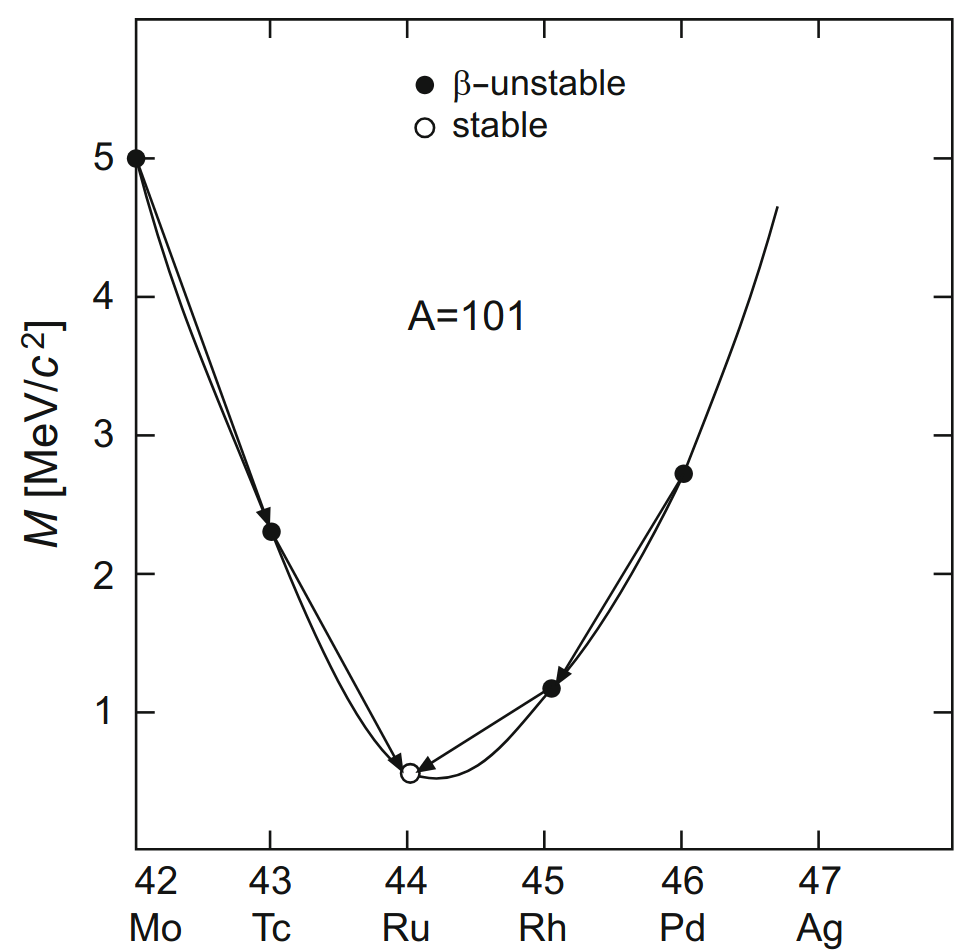
\includegraphics[width=0.45\textwidth]{iso-chain-odd.png}
	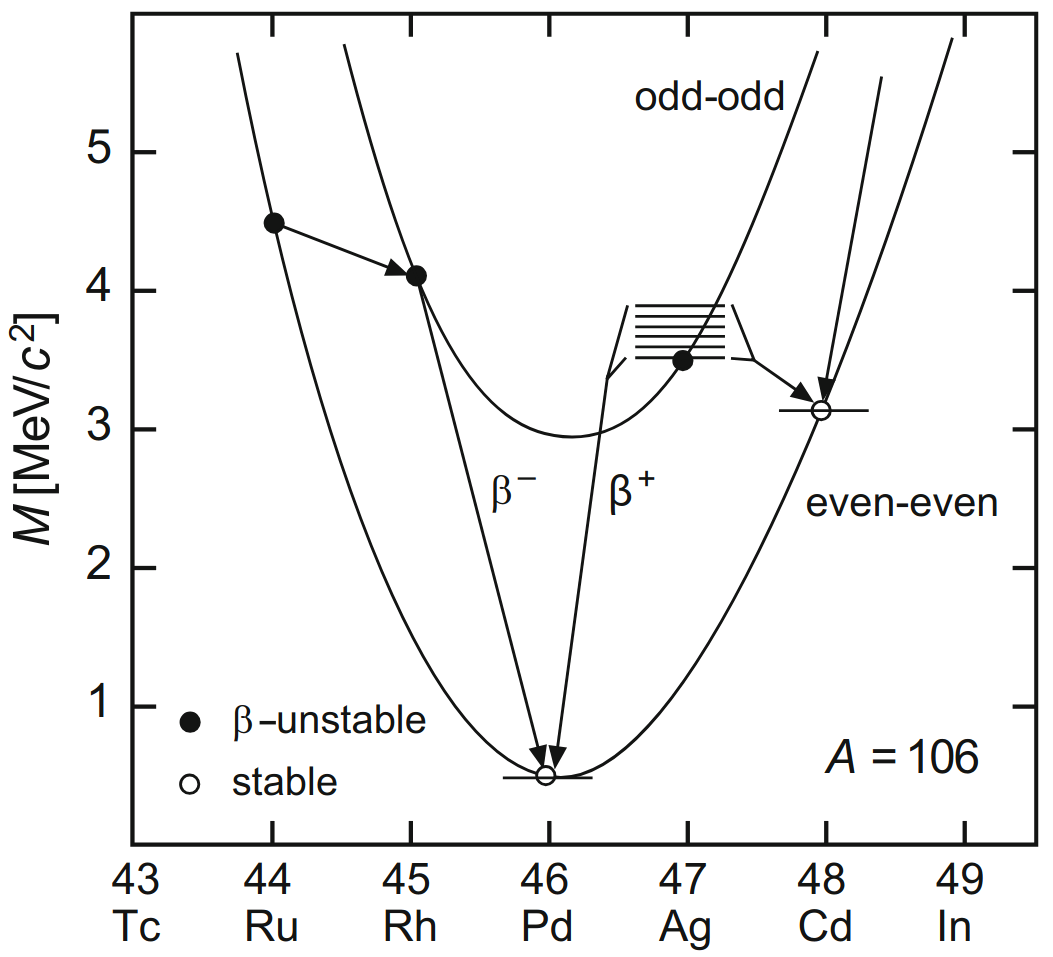
\includegraphics[width=0.45\textwidth]{iso-chain-even.png}
	\caption{Isotopic chain with $ A = 101 $ and $ A = 106 $.}
	\label{iso-chain}
\end{figure}

Tendenzialmente, i nuclidi instabili si riconducono alla stabilità tramite decadimento $ \beta $, sia $ p^+ \rightarrow n $ che $ n \rightarrow p^+ $. In casi particolari, alcuni nuclidi con $ N $ e $ Z $ dispari possono decadere con un doppio decadimento $ \beta $.\\
La formula semi-empirica ha un ottimo accordo coi dati sperimentali per i nuclei pesanti, con errori di circa $ \pm 1\% $, mentre per i nuclei leggeri sono presenti alcune discrepanze: a basso $ A $, il modello a goccia diventa poco accurato.\\
Inoltre, va notato che il modello presenta delle grosse incertezze (sia per le masse che per le abbondanze isotopiche) per isotopi senza valori sperimentali delle masse.

\subsection{Momento angolare e spin}

Gli elettroni negli atomi si dispongono su orbite quantizzate dai numeri quantici dell'elettrone:
\begin{itemize}
	\item numero quantico principale $ n \in \N $, determina il livello energetico dell'elettrone;
	\item numero quantico orbitale $ \ell \in \left[ 0, n-1 \right] \subset \N $, determina il momento angolare orbitale dell'elettrone;
	\item numero quantico magnetico $ m \in \left[ -\ell, \ell \right] \subset \N $, legato alla proiezione del momento angolare sull'asse $ z $ (convenzione);
	\item numero quantico di spin $ s = \pm \frac{1}{2} $, determinante lo spin dell'elettrone.
\end{itemize}
Si ricordi che lo spin, sebbene rappresentato come una rotazione su sé stesso dell'elettrone, è un concetto puramente quanto-meccanico introdotto da Dirac: l'elettrone è privo di struttura interna, quindi non può ruotare su sé stesso.\\
Data la dualità onda-particella, gli elettroni non sono localizzati nello spazio, ma sono caratterizzati da distribuzioni di probabilità che determinano la probabilità d'interazione di un elettrone in un singolo punto: queste distribuzioni sono determinate dalla funzione d'onda dell'elettrone, la quale è ricavata risolvendo l'equazione di Schrödinger per l'atomo considerato, ed in particolare si ha $ P(x) = \abs{\psi(\ve{x})}^2 $.\\
Per l'atomo più semplice, $ \ch{^1 H} $, si trova:
\begin{equation}
	\psi(r,\theta,\phi) = R_{n,\ell,m}(r) Y_{\ell}^m(\theta,\phi)
	\label{eq:1.31}
\end{equation}
dove $ R_{n,\ell,m}(r) $ è la parte radiale della soluzione e $ Y_{\ell}^m(\theta,\phi) $ quella angolare, data dalle armoniche sferiche:
\begin{equation}
	Y_{\ell}^m(\theta,\phi) = \sqrt{\frac{(2\ell+1)(\ell-m)!}{4\pi(\ell+m)!}} e^{im\phi} P_{\ell}^m(\cos\theta)
	\label{eq:1.32}
\end{equation}
Le deistribuzioni di probabilità per i primi orbitali dell'atomo di $ \ch{^1 H} $ sono plottate in Fig. \ref{hyd-pd}.
\begin{figure}
	\centering
	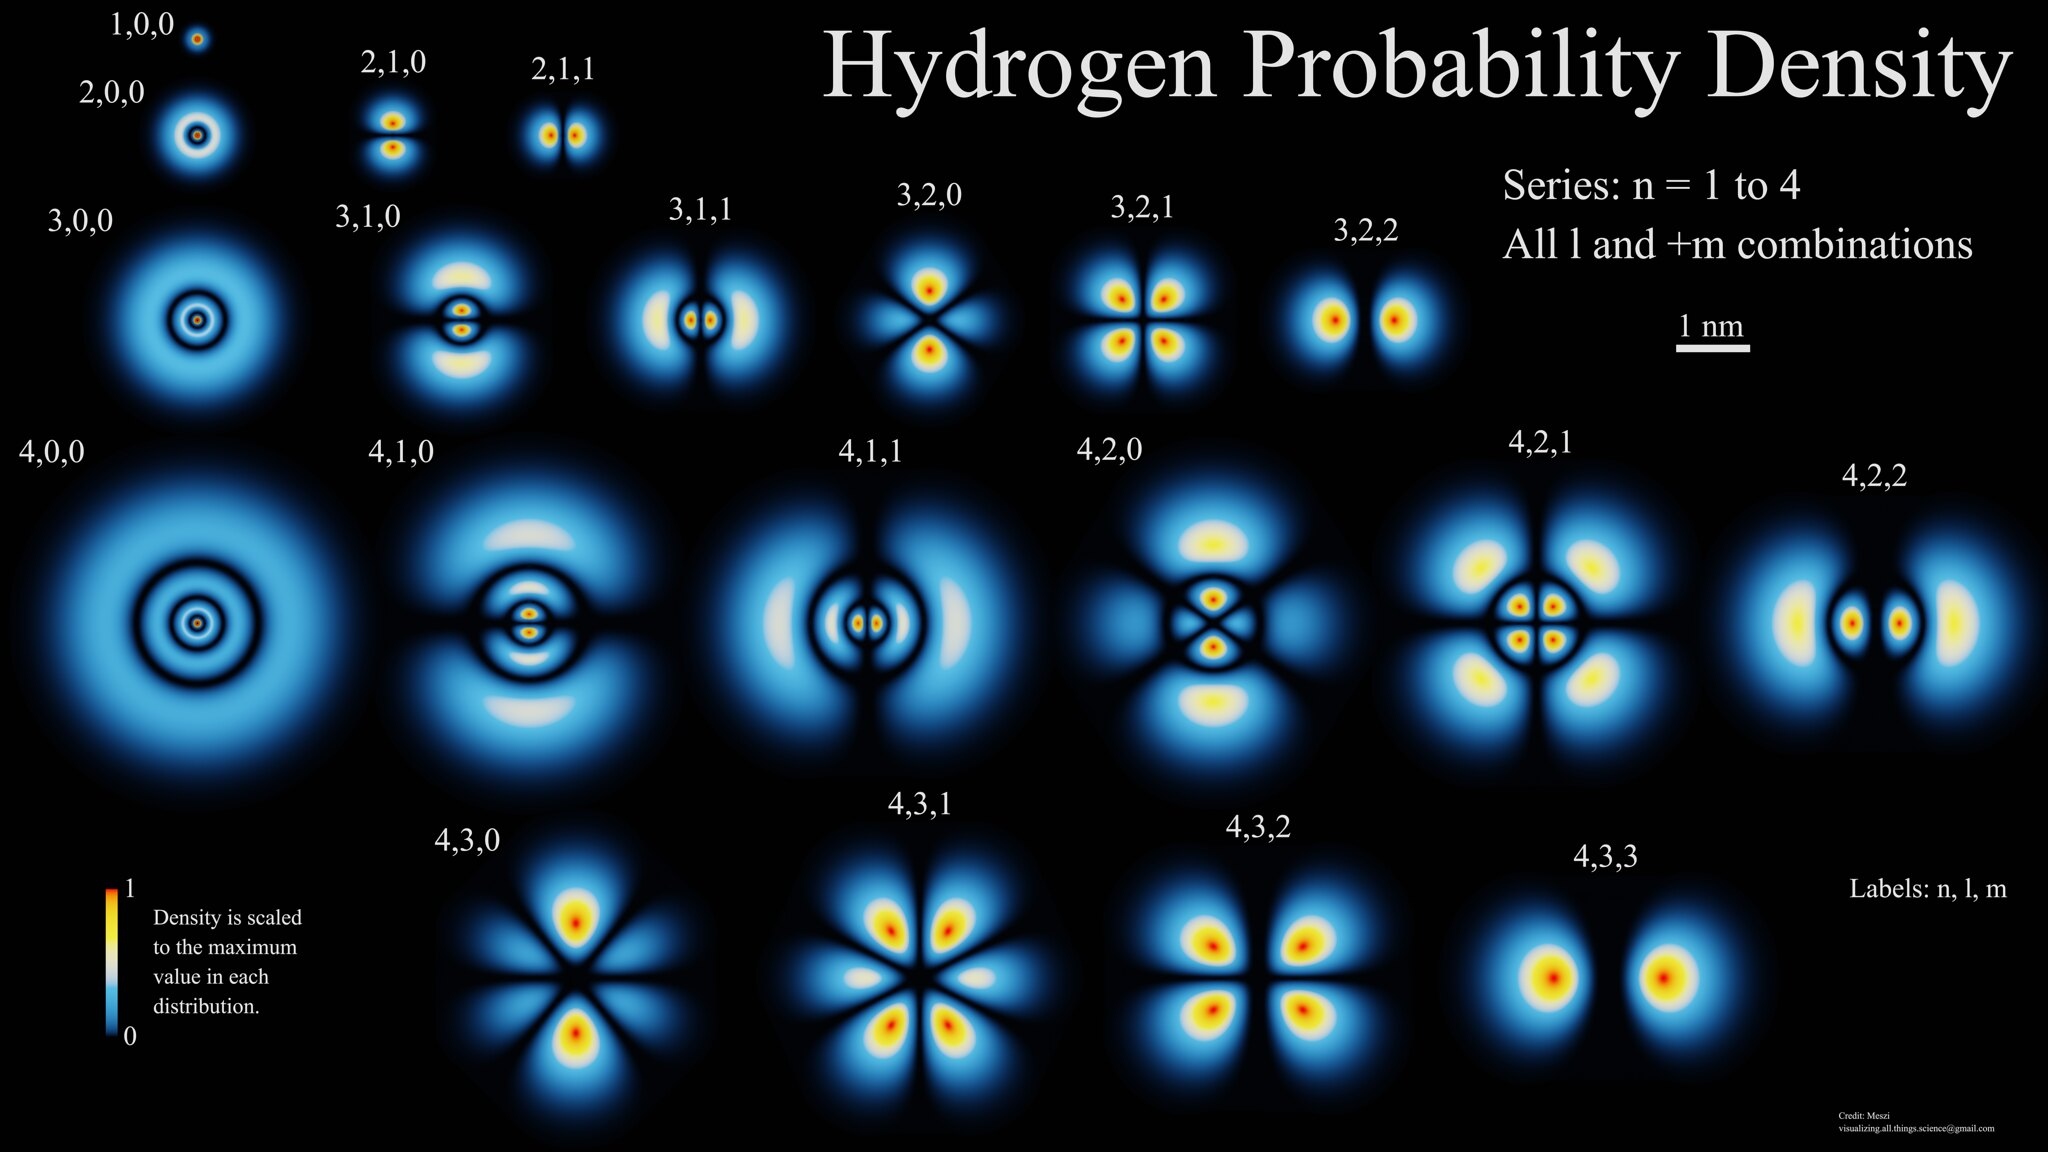
\includegraphics[width=\textwidth]{hydrogen-pd.png}
	\caption{Probability distributions for $ \ch{^1 H} $ atom.}
	\label{hyd-pd}
\end{figure}

Lo stesso modello adottato per gli elettroni è stato adottato anche per quanto riguarda protoni e neutroni nel nucleo: in questo caso, essendo i nucleoni dotati di struttura interna, ha senso immaginare lo spin come il momento angolare associato ad una rotazione del nucleone su sé stesso, basti ricordare che il suo momento angolare $ \ve{J} = \ve{L} + \ve{S} $ è dato dalla somma del momento angolare orbitale e di quello di spin.\\
Prendendo il nucleo nel suo insieme, analogamente al modello elettronico, è possibile avere una stratificazione di densità di probabilità in orbite nucleoniche, separate per protoni e neutroni; il momento angolare nucleare è dato dalla somma dei momenti angolari dei vari nucleoni: $ \ve{J} = \sum_i \ve{J}_i $.

\subsubsection{Parità}

L'operatore parità $ \mathcal{P} $ riflette le posizioni rispetto all'origine: $ \ve{r} \mapsto -\ve{r} $. In coordinate cartesiane, ciò corrisponde a $ (x,y,z) \mapsto (-x,-y-z) $ mentre in coordiante sferiche $ (r,\theta,\phi) \mapsto (r,\pi-\theta,\phi+\pi) $. Applicato alle armoniche sferiche:
\begin{equation}
	\mathcal{P}Y_{\ell}^m(\theta,\phi) = Y_{\ell}^m(\pi-\theta,\phi+\pi) = \left( -1 \right)^{\ell} Y_{\ell}^m(\theta,\phi)
	\label{eq:1.33}
\end{equation}
Si distinguono stati con parità positiva, tali per cui $ \mathcal{P}\psi = \psi $ ($ \ell = 0,2,4,\dots $), e stati a parità negativa, per cui $ \mathcal{P}\psi = -\psi $ ($ \ell = 1,3,5,\dots $). La funzione d'onda di un insieme di particelle è dato dal prodotto delle singole funzioni d'onda, quindi uno stato nucleare ha una parità $ \pi $ ben definita, dal prodotto delle parità di ciascun nucleone: in generale, si indica lo stato nucleare con $ I^{\pi} $, dove $ I $ è il numero di spin del nuclide: questo è la somma in modulo del momento angolare di ciascun nucleone, ovvero $ I = \sum_i J_i $, dunque può assumere una vasta gamma di valori data dal complesso coupling dei vari momenti angolari.
Ad esempio, per $ \ch{^1 H} $ può essere solo $ I = \frac{1}{2} $, mentre per $ \ch{^2 H} $ si può avere $ I = 0,1 $. In generale, per i nuclidi pari-pari $ I = 0 $ a causa del coupling in coppie di spin opposto dei nucleoni, mentre nei nuclidi dispari-dispari sopravvivono nucleoni spaiati che generano uno spin intero; negli altri casi (pari-dispari e dispari-pari) lo spin è semi-intero.\\
Il modulo dello spin nucleare è pari a:
\begin{equation}
	L = \hbar \sqrt{I(I+1)}
	\label{eq:1.34}
\end{equation}
La proiezione di dello spin nucleare su un generico asse $ z $ è $ L_z = \hbar m_I $, con $ m_I \in \left[ -I, I \right] \subset \N $.

\subsubsection{Momento magnetico}

Approssimando l'elettrone come una carica distribuita in orbita circolare a distanza $ r $ dal nucleo con velocità $ v $, si può associare ad esso un momento di dipolo magnetico:
\begin{equation}
	\mu_e = \frac{-e}{T} S = - \frac{ev}{2\pi r} \pi r^2 = - \frac{1}{2} e v r = \frac{-e}{2 m_e} L_z
	\label{eq:1.35}
\end{equation}
In generale, è possibile scrivere:
\begin{equation}
	\mu_{\ell} = g_{\ell} \mu \ell
	\label{eq:1.36}
\end{equation}
dove $ g_{\ell} $ è il fattore $ g $ orbitale, che vale $ g_{\ell} = -1 $ per l'elettrone, $ g_{\ell} = +1 $ per il protone e $ g_{\ell} = 0 $ per il neutrone, mentre $ \mu $ può assumere i valori $ \mu_B \defeq \frac{e\hbar}{2m_e} = 5.7884\cdot10^{-5}\ev/\text{T} $ per l'elettrone (magnetone di Bohr) o $ \mu_N = \frac{e\hbar}{2m_p} = 3.1525\cdot10^{-8}\ev/\text{T} $ per il protone (magnetone nucleare). Si vede chiaramente che il momento magnetico elettronico è preponderante su quello nucleare.\\
Analogamente, si può associare un momento magnetico anche allo spin:
\begin{equation}
	\mu_s = g_s \mu s
	\label{eq:1.37}
\end{equation}
dove $ g_s $ è il fattore $ g $ di spin, pari in modulo a 2 per particelle con spin $ \frac{1}{2} $ prive di struttura. Sperimentalmente si osserva:
\begin{align*}
	\mu_s &= -2.002319\, \mu_B s \qquad\text{(elettrone)} \\
	\mu_s &= +5.585691\, \mu_B s \qquad \text{(protone)} \\
	\mu_s &= -3.826084\, \mu_B s \qquad \text{(neutrone)} \\
\end{align*}
Questa è una delle dimostrazioni sperimentali che, a differenza dell'elettrone, i nucleoni non sono structureless.\\
È possibile definite il $ g $-factor $ g_j $ come:
\begin{equation}
	\ve{\mu}_j = g_{\ell} \mu \ve{L} + g_s \mu \ve{S} \eqdef g_j \mu \ve{J}
	\label{eq:1.38}
\end{equation}
Analiticamente, si trova (definendo $ J_z = \hbar j $):
\begin{equation}
	g_j = \frac{1}{2} \left( g_{\ell} + g_s \right) + \frac{1}{2} \frac{\ell (\ell + 1) - s (s + 1)}{j (j + 1)} \left( g_{\ell} - g_s \right)
	\label{eq:1.39}
\end{equation}
detto nuclear $ g $-factor. Si può anche generalizzare al momento magnetico di una generale coppia di momenti angolari soggetti a coupling tali per cui $ J_{1,z} = \hbar j_1 $ e $ J_{2,z} = \hbar j_2 $:
\begin{equation}
	g_j = \frac{1}{2} \left( g_1 + g_2 \right) + \frac{1}{2} \frac{j_1 (j_1 + 1) - j_2 (j_2 + 1)}{j (j + 1)} \left( g_1 - g_2 \right)
	\label{eq:1.40}
\end{equation}

\paragraph{Quark confinement model}

L'Eq. \ref{eq:1.40} può essere utilizata per dare validità al modello a quark dei nucleoni, secondo il quale il protone è composto da due quark up ed un quark down, mentre il neutrone da due quark down ed un quark up.\\
Il quark up ha spin $ s = \frac{1}{2} $, carica $ q = +\frac{2}{3}e $ e massa $ m_u \approx \frac{1}{3}m_p $, mentre il quark down ha $ s = \frac{1}{2} $, $ q = -\frac{1}{3}e $ e $ m_d \approx \frac{1}{3}m_p $; assumendoli entrambi structureless:
\begin{align*}
	\mu_u &= 2 \frac{\frac{2}{3} e}{2 \frac{1}{3}m_p} \hbar s = 4 \mu_N s \\
	\mu_d &= 2 \frac{-\frac{1}{3} e}{2 \frac{1}{3}m_p} \hbar s = -2 \mu_N s \\
\end{align*}
dunque è possibile definire $ g_u = +4 $ e $ g_d = -2 $. Calcolando i momenti magnetici dei nucleoni dal coupling dei momenti magnetici dei quark:
\begin{equation*}
	\begin{split}
		g_{uu} &= \frac{1}{2} (4 + 4) + \frac{1}{2} \frac{\frac{1}{2} \left( \frac{1}{2} + 1 \right) - \frac{1}{2} \left( \frac{1}{2} + 1 \right)}{1 (1 + 1)} \left( 4 - 4 \right) = +4\\
		       &\Longrightarrow g_p \equiv g_{uud} = \frac{1}{2} (4 - 2) + \frac{1}{2} \frac{1 \left( 1 + 1 \right) + \frac{1}{2} \left( \frac{1}{2} + 1 \right)}{\frac{1}{2} \left( \frac{1}{2} + 1 \right)} (4 + 2) = +6\\
		g_{dd} &= \frac{1}{2} (-2 -2) + \frac{1}{2} \frac{\frac{1}{2} \left( \frac{1}{2} + 1 \right) - \frac{1}{2} \left( \frac{1}{2} + 1 \right)}{1 (1 + 1)} \left( -2 +2 \right) = -2\\
		       &\Longrightarrow g_n \equiv g_{ddu} = \frac{1}{2} (-2 + 4) + \frac{1}{2} \frac{1 \left( 1 + 1 \right) + \frac{1}{2} \left( \frac{1}{2} + 1 \right)}{\frac{1}{2} \left( \frac{1}{2} + 1 \right)} (-2 -4) = -4\\
	\end{split}
\end{equation*}
Questi valori approssimativi (poiché modello approssimativo) sono in accordo con i valori sperimentali $ g_p = +5.58 $ e $ g_n = -3.82 $.\\
Se ci si riduce a considerare solo nuclei con $ A $ dispari, si trova:
\begin{equation}
	\langle \mu_z \rangle =
	\begin{cases}
		\left[ g_{\ell} \left( j - \frac{1}{2} \right) + \frac{1}{2} g_s \right] \mu_N & j = \ell - \frac{1}{2} \\
		\left[ g_{\ell} \left( j + \frac{3}{2} \right) + \frac{1}{2} g_s \right] \frac{j}{j + 1} \mu_N & j = \ell + \frac{1}{2}
	\end{cases}
	\label{eq:1.41}
\end{equation}
Queste, dette linee di Schmidt, costituiscono gli estremi per il valore del momento magnetico del nuclide, ma non fittano i dati sperimentali (se non moltiplicati per un fattore scala): questo è dovuto al fatto che il modello adottato assuma che il momento magnetico del nuclide sia dato dall'unico nucleone spaiato (a causa del pairing in coppie di spin nullo). In realtà, sebbene spaiato, il singolo nucleone interagisce comunque con i nucleoni nelle sue vicinanze e col mezzo nucleare, dunque il modello adottato è solo approssimativo.

\paragraph{Risonanza magnetica nucleare}

La MRI (Magnetic Resonance Imaging) o NMR (Nuclear Magnetic Resonance) è una tecnica di imaging utilizzata per avere immagini dei tessuti corporei ad alta risoluzione. Il suo funzionamento si basa sullo spin splitting.\\
Quando un nuclide viene posto in un campo magnetico abbastanza intenso, c'è un'interazione tra il momento magnetico nucleare ed il campo magnetico esterno: ciò fa sí che si rompa la degenerazione sui valori dello spin, con importanti conseguenze dal punto di vista applicativo.\\
Prendendo il caso di un tessuto umano, i nucleoni in esso sono distribuiti con spin casuali, ma introducendo il tessuto in un forte campo magnetico essi si allineano alla direzione del campo: di conseguenza, essi precedono con frequenza di Larmor \footnotemark attorno alla direzione del campo e, dato che lo spin è quantizzato $ s = \pm\frac{1}{2} $, la precessione avviene in due direzioni diverse, una parallela ed una antiparallela al campo (splitting).\\
Facendo oscillare il campo magnetico ad una specifica frequenza, determinata dalla differenza di energia tra i due stati splittati, è possibile indurre una transizione dallo stato con energia più bassa a quello con energia più alta (spin flip): una volta spento il campo esterno, il sistema tende a tornare alla sua configurazione d'equilibrio, ovvero allo stato di energia più bassa. Questa transizione avviene emettendo radiazione rilevabile, con tempi di rilassamento dipendenti dal tessuto.\\
La MRI porta il sistema in stati eccitati, riorientandone gli spin, e ne rileva il rilassamento con emissione di radiazione, dunque non viene utilizzata nessuna forma di radiazione sul tessuto (come per esempio i raggi X): questo tipo di esame non è nocivo.

\footnotetext{La frequenza di Larmor è la frequenza di precessione del momento magnetico di un oggetto attorno ad un campo magnetico esterno; essa è pari a $ \omega_L = \abs{\gamma B} $, con $ \gamma \defeq \frac{\mu_B}{L} $ il rapporto giroscopico dell'oggetto considerato (es. $ \gamma_e = g_e\frac{-e}{2m_e} $ per l'elettrone).}












\chapter{Decadimenti}
\selectlanguage{italian}

\section{Radioattività}

I primi indizi verso la radioattività sono derivati dalla rilevazione dei raggi X: questi sono onde elettromagnetiche, ovvero fotoni, generate da transizioni di elettroni tra livelli energetici ($ \Delta E_e = \hbar \omega $); questi dunque non sono processi nucleari, dato che avvengono all'interno della nube elettronica dell'atomo.\\
Quando si parla di radioattività in senso stretto, però, si fa riferimento ai decadimenti dei nuclidi.

\subsection{Decadimenti radioattivi}

I decadimenti radioattivi sono processi in cui un nuclide stabile raggiunge una configurazione con energia più bassa emettendo spontaneamente radiazione.\\
Utilizzando un campo magnetico, Rutherford riuscì a distinguere tre tipologie di radiazione, e dunque di decadimenti radioattivi:
\begin{enumerate}
  \item decadimento $ \alpha $, in cui la radiazione è costituita da un nucleo di $ \ch{^4_2 He} $ ed è poco penetrante, coinvolge l'interazione elettromagnetica e quella forte;
  \item decadimento $ \beta^{\pm} $, in cui la radiazione è costituita da un $ e^{\pm} $ ed è mediamente penetrante, coinvolge l'interazione debole:
    \begin{itemize}
      \item decadimento $ \beta^- $: $ n \rightarrow p^+ + e^- + \bar{\nu}_e $;
      \item decadimento $ \beta^+ $: $ p^+ \rightarrow n + e^+ + \nu_e $;
    \end{itemize}
  \item decadimento $ \gamma $, in cui la radiazione è costituita da un fotone con energia dell'ordine delle decine di MeV, dunque estremamente penetrante.
\end{enumerate}
A questi si aggiunge la cattura elettronica, un decadimento in cui un nuclide proton-rich cattura un elettrone dalle shell interne dell'atomo, seguendo la reazione $ p^+ + e^- \rightarrow n + \nu_e $, emettendo raggi X a seguito del rimpiazzo dell'elettrone interno con uno dalle shell esterne.

\subsection{Energy balance}

Un decadimento radioattivo può essere visto come un caso particolare di reazione nucleare; è quindi possibile definire il $ Q $-value del decadimento come la differenza di energia a riposo (massa) tra reagenti (nuclide instabile) e prodotti, così da poter stabilire qualora esso sia possibile, ovvero spontaneo, con la condizione $ Q > 0 $.\\
In particolare, si definiscono i $ Q $-values dei seguenti decadimenti:
\begin{enumerate}
  \item decadimento $ \alpha $: $ Q_{\alpha} \equiv \left[ M(Z,A) - M(Z-2,A-4) - m(\ch{^4_2 He}) \right] c^2 $;
  \item decadimento $ \beta^- $: $ Q_{\beta^-} \equiv \left[ M(Z,A) - M(Z+1,A) - m_e \right] c^2 $;
  \item decadimento $ \beta^+ $: $ Q_{\beta^+} \equiv \left[ M(Z,A) - M(Z-1,A) - m_e \right] c^2 $;
  \item electron capture: $ Q_{e} \equiv \left[ M(Z,A) + m_e - M(Z-1,A) \right] c^2 $;
\end{enumerate}
Si vede subito che $ Q_e > Q_{\beta^+} $: di conseguenza, nell'electron capture i prodotti di decadimento hanno maggior energia cinetica disponibile, inoltre ci sono dei casi in cui può avvenire l'electron capture ma non il decadimento $ \beta^+ $.

\subsection{Radioactive decay law}

Il processo di decadimento ha natura aleatoria, dunque va trattato in maniera statistica.\\
Il numero di decadimenti al secondo è proporzionale al numero di nuclidi radioattivi:
\begin{equation}
	- \frac{dN}{dt} = \lambda N(t)
	\label{eq:2.1}
\end{equation}
Si trova quindi la legge di decadimento esponenziale:
\begin{equation}
	N(t) = N_0 e^{-\lambda t}
	\label{eq:2.2}
\end{equation}
Si definisce inoltre il decay rate (o activity) come $ A(t) \defeq \lambda N(t) $, misurato in Bequerel $ 1\,\text{Bq} = 1 \,\text{decay}/\text{s} $ o in Curie $ 1\,\text{Ci} = 3.7\cdot10^{10}\,\text{Bq} $ (activity di $ 1\,\text{g} $ di radio). Si definiscono inoltre la half-life $ t_{1/2} \equiv \frac{\ln 2}{\lambda} $ e la vita media $ \tau = \frac{1}{\lambda} $ rispettivamente come il tempo dopo il quale il campione si è ridotto di $ \frac{1}{2} $ e di $ \frac{1}{e} $: si ha $ t_{1/2} \approx 0.693 \tau < \tau $.\\
Per i decay rates si trova facilmente che, definendo $ A_0 \equiv \lambda N_0 $:
\begin{equation}
	A((n+1)t) = A(t) \left( \frac{A(t)}{A_0} \right)^n
	\label{eq:2.3}
\end{equation}
Nel caso di una miscela di radioisotopi, è possibile risalire alle singole costanti di decadimento nel caso in cui le vite medie siano molto diverse, poiché quando la specie con la $ \tau $ più corta è completamente decaduta si può misurare direttamente la $ \lambda $ dell'altra specie, per poi risalire a quella della prima tramite la differenza delle activities.

\subsubsection{Decay branches}

Può capitare che lo stesso nuclide radioattivo possa decadere in due o più modi differenti, detti decay branches: detta $ \lambda_k $ la costante di decadimento parziale della $ k $-esima branch, nel caso di $ n $ branches si ha:
\begin{equation}
	\lambda \equiv \lambda_1 + \dots + \lambda_n
	\label{eq:2.4}
\end{equation}
e questa costante totale è l'unica che si osserva, anche quando si rileva una sola delle branches. Si definiscono i branching ratios come $ B_k \defeq \frac{\lambda_k}{\lambda} $.

\subsubsection{Decay chains}

Spesso, in un decadimento radioattivo, capita che anche i prodotti siano radiaottivi: ciò dà vita ad una catena di decadimenti $ N_1 \xrightarrow{\lambda_1} N_2 \xrightarrow{\lambda_2} N_3 \dots $, dove le $ \lambda_k $ sono diverse tra loro.\\
Una decay chain è descritto da un sistema di coupled differential equations. Nel caso, ad esempio, di un doppio decadimento (quindi con prodotto $ N_3 $ stabile):
\begin{equation}
	\begin{cases}
		\dot{N}_1 = - \lambda_1 N_1 \\
		\dot{N}_2 = \lambda_1 N_1 - \lambda_2 N_2 \\
		\dot{N}_3 = \lambda_2 N_2
	\end{cases}
	\quad\Longrightarrow\quad
	\begin{cases}
		N_1(t) = N_0 e^{-\lambda_1 t} \\
		N_2(t) = \frac{\lambda_1}{\lambda_1 + \lambda_2} N_0 \left( e^{-\lambda_1 t} - e^{-\lambda_2 t} \right) \\
		N_3(t) = \frac{\lambda_1 \lambda_2}{\lambda_1 + \lambda_2} N_0 \left( \frac{1 - e^{-\lambda_1 t}}{\lambda_1} - \frac{1 - e^{-\lambda_2 t}}{\lambda_2} \right)
	\end{cases}
	\label{eq:2.5}
\end{equation}
La soluzione generale al caso di $ n $ decadimenti è dato dall'\textit{equazione di Bateman}:
\begin{equation}
	N_k(t) = \sum_{i = 1}^{k} \left[ N_0^{(i)} \left( \prod_{j = 1}^{k-1} \lambda_j \right) \left( \sum_{j = i}^{k} \frac{e^{-\lambda_j t}}{\prod_{p=i, p\neq j}^{k} (\lambda_p - \lambda_j)} \right) \right]
	\label{eq:2.6}
\end{equation}

\paragraph{Equilibrio radioattivo} Si parla di equilibrio radioattivo quando la specie radioattiva madre e quella figlia hanno la stessa attività, ovverosia quando la specie figlia decade allo stesso rate a cui è prodotta. In una decay chain, l'equilibrio radioattivo può instaurarsi tra ciascuna coppia di nuclidi della catena: la condizione generale da soddisfarre è che $ (t_{1/2})_{\text{madre}} > (t_{1/2})_{\text{figlia}} $.\\
In particolare, si parla di:
\begin{enumerate}
	\item equilibrio transiente: si ha quando $ (t_{1/2})_{\text{madre}} \approx (t_{1/2})_{\text{figlia}} $, dunque, dopo un periodo di transienza iniziale, l'activity della specie madre e quella della specie figlia diventano uguali;
	\item equilibrio secolare: si ha quando $ (t_{1/2})_{\text{madre}} \rightarrow \infty $ (comparabile all'età della Terra), dunque la sua activity è praticamente costante; di conseguenza, dopo un certo periodo di tempo, anche l'activity della specie figlia diventerà costante e pari a quella della specie madre (si vede analiticamente dall'Eq. 2.5 ponendo $ \lambda_1 \ll \lambda_2 $). Si parla di equilibrio secolare anche quando, più genericamente, $ (t_{1/2})_{\text{madre}} \gg (t_{1/2})_{\text{figlia}} $.
\end{enumerate}

\paragraph{Serie radioattive naturali}

Ci sono 4 serie decay chains naturali principali, tutte composte da decadimenti $ \alpha $ e $ \beta^- $:
\begin{enumerate}
  \item serie del torio: inizia col $ \ch{^{232} Th} $ e termina col $ \ch{^{208} Pb} $, il decadimento col tempo di dimezzamento più lungo è $ \ch{^{232} Th} \rightarrow \ch{^{228} Ra} $ con $ t_{1/2} = 14 \,\text{Gy} $;
  \item serie dell'uranio: inizia col $ \ch{^{238} U} $ e termina col $ \ch{^{206} Pb} $, il decadimento col tempo di dimezzamento più lungo è $ \ch{^{238} U} \rightarrow \ch{^{234} Th} $ con $ t_{1/2} = 4.5 \,\text{Gy} $;
  \item serie del plutonio: inizia col $ \ch{^{239} Pu} $ e termina col $ \ch{^{207} Pb} $, il decadimento col tempo di dimezzamento più lungo è $ \ch{^{235} U} \rightarrow \ch{^{231} Th} $ con $ t_{1/2} = 0.71 \,\text{Gy} $;
  \item serie del nettunio: inizia col $ \ch{^{237} Np} $ e termina col $ \ch{^{209} Bi} $, il decadimento col tempo di dimezzamento più lungo è $ \ch{^{237} Np} \rightarrow \ch{^{233} Pa} $ con $ t_{1/2} = 2.3 \,\text{My} $;
\end{enumerate}
Quest'ultima serie non è più osservabile in natura poiché la sua vita media non è comparabile con l'età della Terra, a differenza delle altre tre.

\paragraph{Carbon dating}

Il $ \ch{^{14}C} $ è un isotopo radioattivo del carbonio con $ t_{1/2} = 5730\,\text{y} $; nonostante questa vita media relativamente corta, esso è prodotto continuamente grazie ai raggi cosmici in atmosfera tramite neutron capture: $ \ch{^{14}N} + n \rightarrow \ch{^{14}C} + p^+ $; una volta assorbito dai sistemi biologici, esso decade per decadimento $ \beta^- $: $ \ch{^{14}C} \rightarrow \ch{^{14}N} + e^- + \bar{\nu}_e $.\\
Misurata la specific activity $ a $ del campione da datare, si può risalire al time since death comparandola alla standard specific activity $ a_0 = 0.266\,\text{Bq}/\text{g} $: $ T = \frac{t_{1/2}}{\ln 2} \ln \frac{a}{a_0} = - 8033\,\text{y} \cdot \ln \frac{a}{a_0} $.\\
L'assunzione fondamentale di questo metodo di datazione è che la concentrazione naturale di $ \ch{^{14}C} $ rimanga costante nel tempo: con la Guerra Fredda questo è diventato un problema, poiché i test nucleari hanno fatto raddoppiare per un periodo tale concentrazione, e solo ultimamente si sta tornando ai livelli precedenti. Inoltre, va notato che il carbon dating è efficacie solo per oggetti non più vecchi di 50'000 anni: per epoche precedenti, sono necessari altre coppie isotopiche, come ad esempio $ \ch{^{40}K} $ - $ \ch{^{40}Ar} $, $ \ch{^{235}U} $ - $ \ch{^{207}Pb} $ o $ \ch{^{238}U} $ - $ \ch{^{208}Pb} $.

\section{Decadimento \texorpdfstring{$ \alpha $}{TEXT}}

Il decadimento $ \alpha $ consiste nell'emissione di un nucleo di $ \ch{^4 He} $ da parte di un nucleo instabile, secondo la reazione:
\begin{equation}
	\ch{^A_Z X_N} \rightarrow \ch{^{A-4}_{Z-2} Y_{N-2}} + \ch{^4_2 He_{2}}
	\label{eq:2.7}
\end{equation}
Questo avviene grazie alla repulsione coulombiana tra nucleo e $ \alpha $, espressa dall'andamento dell'energia potenziale:
\begin{equation}
	U(r) = \frac{2(Z-2)e^2}{4\pi \epsilon_0 r}
	\label{eq:2.8}
\end{equation}
È il decadimento prevalente nei nuclei pesanti: ad elevati $ A $ conviene ridurre la massa del sistema per acquisire maggiore stabilità (si veda Fig. \ref{bind-en}). Per lo stesso motivo, non si osservano decadimenti $ \alpha $ in nuclei più leggeri del $ \ch{^{126}_{62} Sm} $.

\paragraph{Bilancio energetico}

È fondamentale studiare il bilancio energetico del decadimento $ \alpha $: in particolare, esso è possibile quando il $ Q $-value dell'Eq. $ \ref{eq:2.7} $ è positivo. Assumendo che il nuclide instabile sia inizialmente a riposo:
\begin{equation}
	Q = T_{\ch{Y}} + T_{\alpha} = \left( m_{\ch{X}} - m_{\ch{Y}} - m_{\alpha} \right) c^2
	\label{eq:2.9}
\end{equation}
A ciò va aggiunta la conservazione del momento lineare, la quale impone che $ \ve{p}_{\ch{Y}} = -\ve{p}_{\alpha} $, con la quale si trova (trattando non-relativisticamente, dato che i valori tipici sono $ T_{\alpha} \sim 5\mev $):
\begin{equation}
	T_{\alpha} = \frac{m_{\ch{Y}}}{m_{\ch{Y}} + m_{\alpha}} Q \approx \left( 1 - \frac{4}{A} \right) Q
	\label{eq:2.10}
\end{equation}
Dunque $ \alpha $ trasporta circa il $ 98\% $ del $ Q $-value ($ \sim 5\mev $), mentre il restante $ 2\% $ ($ \sim 0.1\mev $) viene trasmesso al nuclide figlio $ \ch{Y} $ come recoil energy (può diventare significativa in decay chains, portando a radioactive material leaks).\\
Si osserva inoltre che, essendo il decadimento $ \alpha $ un decadimento a due corpi, le particelle emesse sono mono-energetiche, ovvero, fissata la specie nucleare che decade, le particelle $ \alpha $ vengono emesse tutte praticamente con la stessa energia fissata dall'Eq. \ref{eq:2.10}. Ciò non vale per i decadimenti a tre o più corpi.

\subsection{Systematics}

Osservazioni sperimentali (condotte originariamente da Geiger e Nuttall) rivelano che, sebbene il processo di decadimento sia fondamentalmente sempre lo stesso, i tempi di dimezzamento possono variare di svariati ordini di grandezza tra le varie specie nucleari, in relazione anche a come varia il $ Q $-value: si va dal $ \ch{^{232}Th} $ con $ t_{1/2} = 14 \,\text{Gy} $ e $ Q = 4.08\mev $ al $ \ch{^{218}Th} $ con $ t_{1/2} = 0.1 \,\mu\text{s} $ e $ Q = 9.85\mev $, ovvero una variazione di 24 ordini di grandezza nella half-life a fronte di un solo fattore 2 nel $ Q $-value.\\
Plottando i dati sperimentali (Fig. \ref{geiger-nuttall}) si osserva un trend che prende il nome di \textit{legge di Geiger-Nuttall}:
\begin{equation}
	\ln t_{1/2} = a(Z) + \frac{b(Z)}{\sqrt{Q}}
	\label{eq:2.11}
\end{equation}
dove $ a $ e $ b $ sono parametri empirici. La conferma teorica di questa legge è stata una delle prime prove della meccanica quantistica.\\
Studiando invece la dipendeza di $ Q $ da $ A $ (Fig. \ref{gn-mass}) si può osservare un'importante discontinuità in corrispondenza di $ N = 126 $, mostrando ancora una volta la presenza di una nuclear shell structure.

\begin{figure}
	\centering
	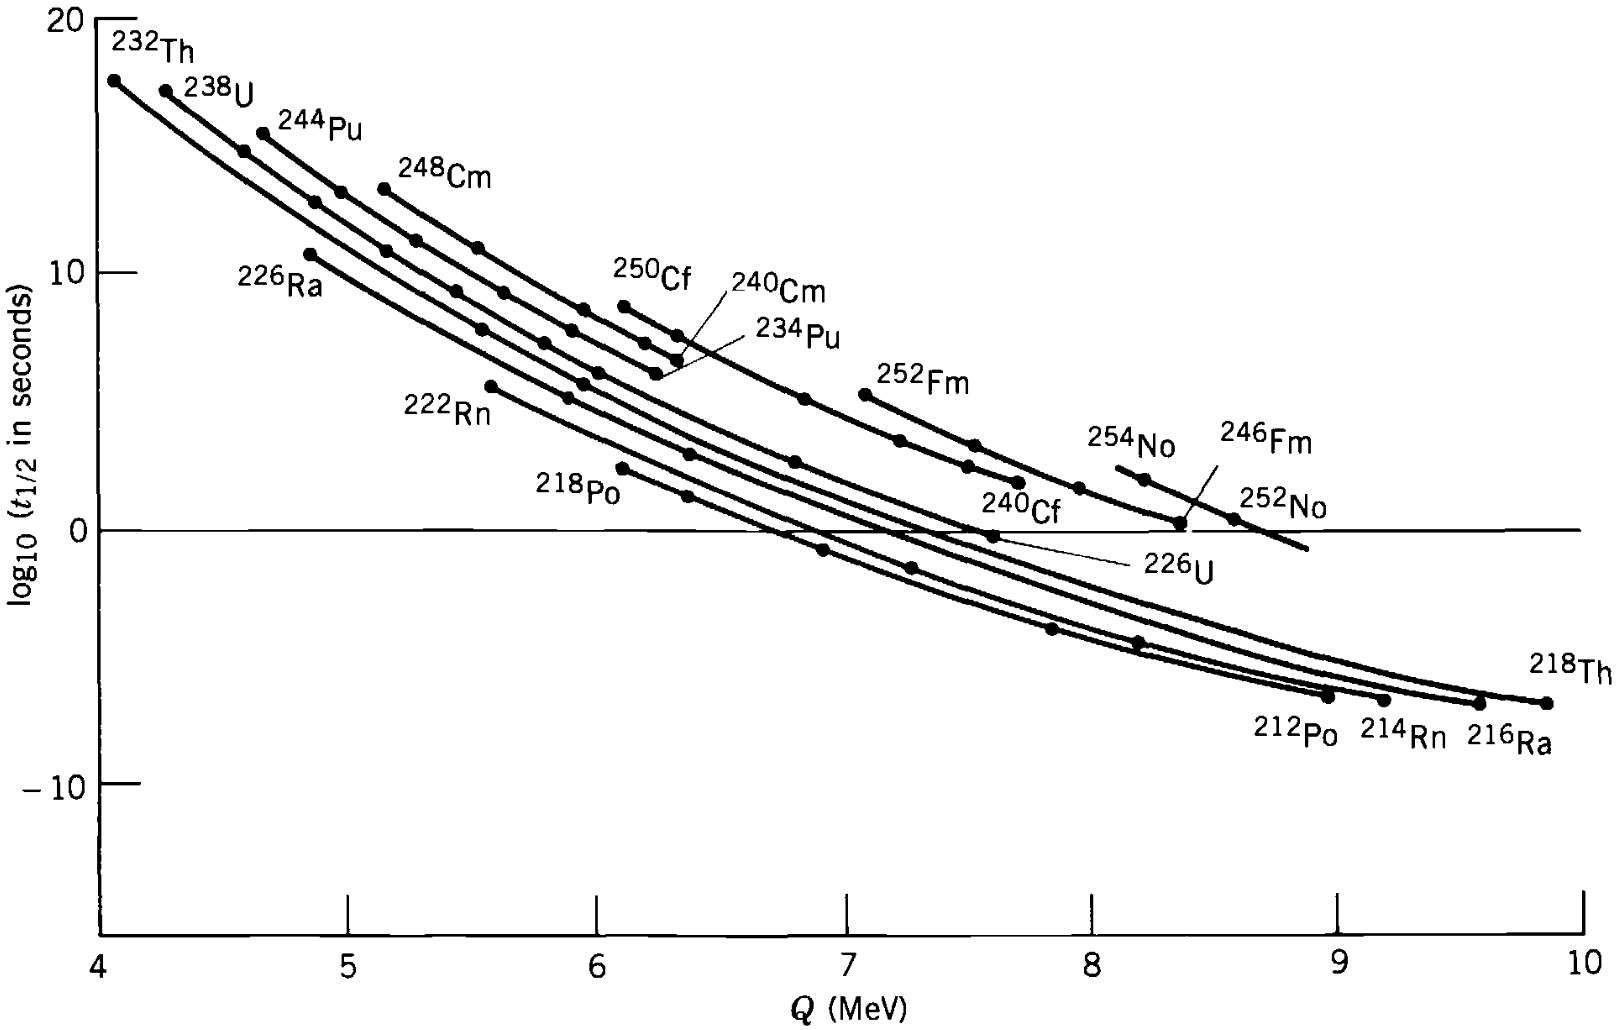
\includegraphics[width=0.75\textwidth]{geiger-nuttall.png}
	\caption{Legge di Geiger-Nuttal in famiglie isotopiche con nuclidi pari-pari.}
	\label{geiger-nuttall}
\end{figure}
\begin{figure}
	\centering
	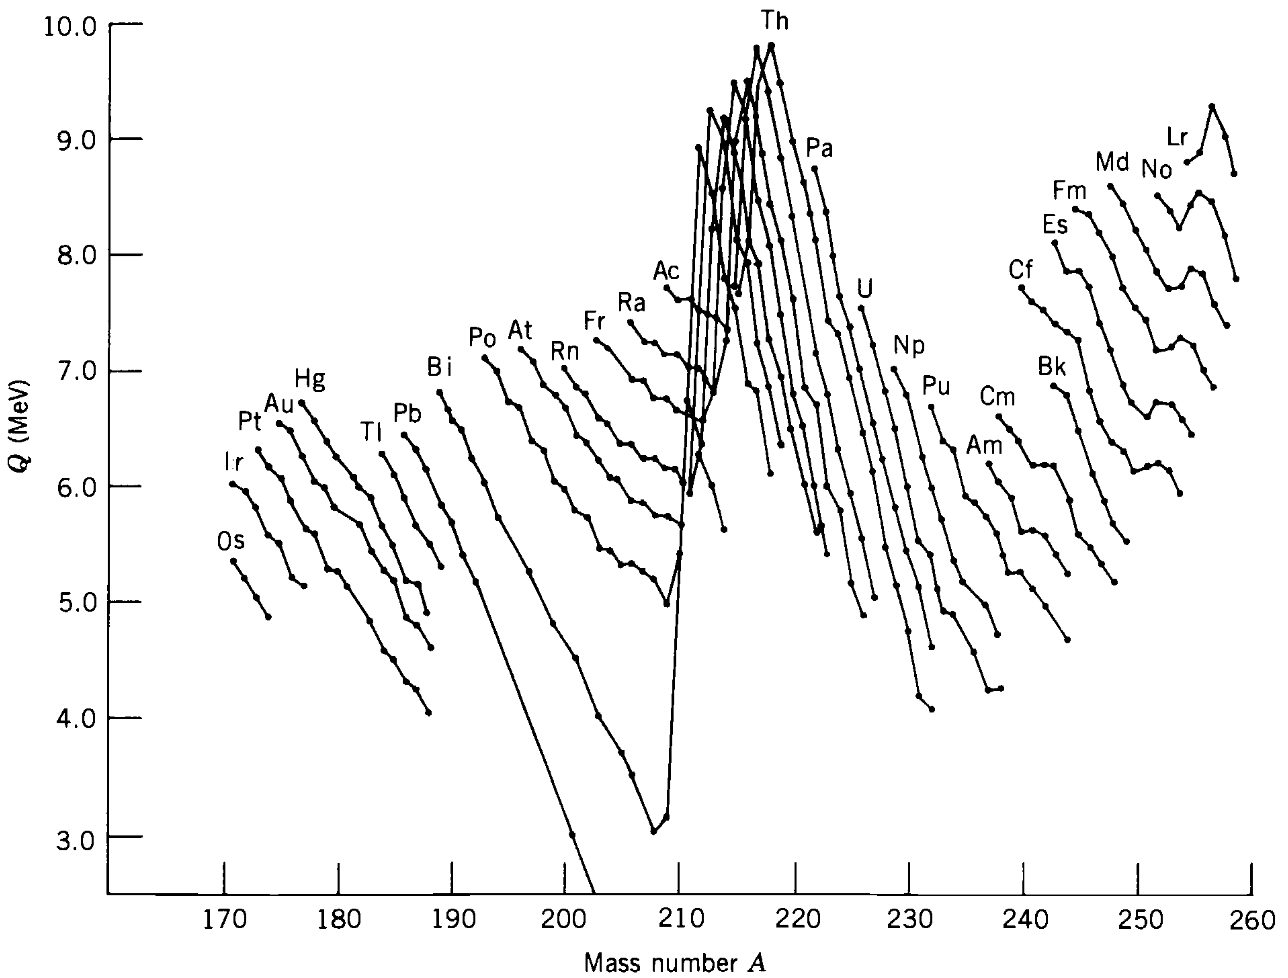
\includegraphics[width=0.75\textwidth]{gn-mass.png}
	\caption{Energia emessa per decadimento $ \alpha $ in famiglie isotopiche.}
	\label{gn-mass}
\end{figure}

\subsection{Teoria di Gamow}

La prima interpretazione teorica del decadimento $ \alpha $ fu data da Gamow nel 1929, qualche anno dopo le osservazioni di Geiger e Nuttall.\\
È possibile pensare alla particella $ \alpha $ come un corpo stabile preformato all'interno del nuclide $ \ch{^A X} $ che periodicamente di viene a trovare sulla superficie del nucleo, ad una distanza $ R \equiv R_{\ch{Y}} + R_{\alpha} $. Il moto della particella $ \alpha $ è determinato dal'energia potenziale d'interazione col nucleo, plottata in Fig. \ref{alpha-pot}, che fu proposta da Gamow essere:
\begin{equation}
	U(r) =
	\begin{cases}
		-V_0 & r < R \\
		\frac{2(Z-2)e^2}{4\pi \epsilon_0 r} & r > R
	\end{cases}
	\label{eq:2.12}
\end{equation}
Il senso fisico di tale espressione è che in prossimità del nucleo a prevalere è la forza nucleare, che ha natura attrattiva, mentre allontanandosi da esso prevale l'interazione coulombiana, che è repulsiva: si vede quindi la presenza di una barriera coulombiana in $ r = R $.\\
Con una trattazione classica la particella $ \alpha $ sarebbe emessa solo se $ E_{\alpha} > U(R) $ e ciò avverrebbe in un tempo comparabile al tempo di attraversamento del nucleo, ovvero $ t \sim R / v_{\alpha} = R \sqrt{2E_{\alpha} / m_{\alpha}} $: stimando $ R \approx 1.2\fm \left( (A - 4)^{1/3} + 4^{1/3} \right) $, per un nucleo con $ A \sim 230 $ e $ Q \sim 4\mev $ si trova $ R \sim 9\fm $ e $ t \sim 10^{-21}\,\text{s} $, ovvero un decadimento praticamente istantaneo. Ciò però non è quello che si osserva sperimentalmente.\\
Quantisticamente, invece, grazie all'effetto tunnel è possibile che anche le particelle $ \alpha $ con $ E_{\alpha} < U(R) $ (cosa che è praticamente sempre, dato che $ U(R) \sim 20\mev $) possono essere emesse con probabilità inderiori e dunque tempi di decadimento più lunghi.\\
È possibile svolgere il calcolo esplicitamente approssimando il potenziale coulombiano tra $ r = R $ ed $ r = R_{\alpha} $ (determinato da $ U(R_{\alpha}) = E_{\alpha} $) come una successione di barriere di potenziale di spessore $ dr $: dalla meccanica quantistica è noto che un'onda (particella) incidente su una barriera di potenziale di spessore $ L $ risulta in un'onda riflessa ed una trasmessa, le cui rispettive distribuzioni di probabilità (funzioni d'onda) sono determinate dai coefficienti di riflessione e trasmissione.

\begin{figure}[!hb]
	\centering
	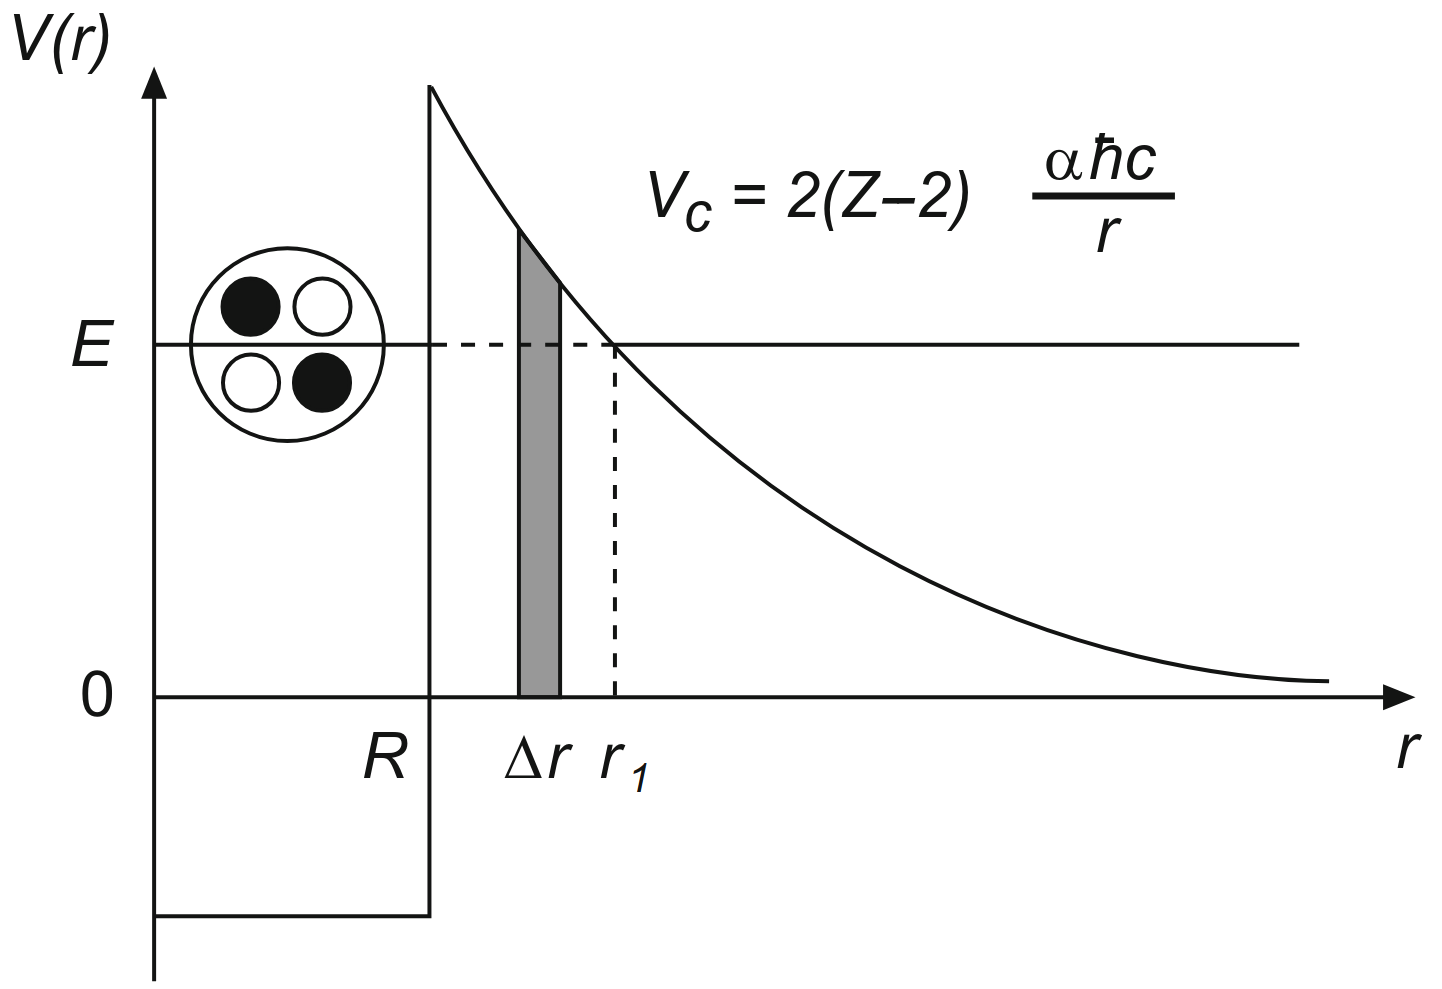
\includegraphics[width=0.60\textwidth]{alpha-pot.png}
	\caption{Potenziale d'interazione per il decadimento $ \alpha $.}
	\label{alpha-pot}
\end{figure}

Nel caso del decadimento $ \alpha $ è d'interesse solo il coefficiente di trasmissione nell'approssimazione $ E \ll V_0 $:
\begin{equation}
	T(E) = \left[ 1 + \frac{U_0^2}{4E (U_0 - E)} \sinh^2 \left( \frac{L}{\hbar} \sqrt { 2m (U_0 - E)} \right) \right]^{-1} \approx \frac{16 E (U_0 - E)}{U_0^2} e^{-2 \frac{L}{\hbar} \sqrt{2m (U_0 - E)}}
	\label{eq:2.13}
\end{equation}
Nel modello approssimato della successione di barriere di potenziale, quindi, si trova una probabilità di tunneling data da:
\begin{equation}
	P(E_{\alpha}) = \exp{\left[ -2 \int_{R}^{R_{\alpha}} dr \frac{1}{\hbar} \sqrt{2 m (U(r) - E_{\alpha}}) \right]} \eqdef e^{-2G}
	\label{eq:2.14}
\end{equation}
dove è stato definito il \textit{fattore di Gamow} $ G $. Svolgendo il calcolo col potenziale in Eq. \ref{eq:2.12} ed approssimando per una thick barrier $ R_{\alpha} \gg R $ (equivalente a $ E_{\alpha} \ll U(R) $, dato che dalla definizione $ R / R_{\alpha} = E_{\alpha} / U(R) $):
\begin{equation}
	\begin{split}
		G(E_{\alpha})
		&= \frac{2 (Z - 2) e^2}{\hbar} \sqrt{\frac{2m_{\alpha}}{E_\alpha}} \left[ \arccos \sqrt{\frac{R}{R_{\alpha}}} - \sqrt{\frac{R}{R_{\alpha}} - \frac{R^2}{R^2_{\alpha}}} \right]\\
		&\approx \frac{2 (Z - 2) e^2}{\hbar} \sqrt{\frac{2m_{\alpha}}{E_{\alpha}}} \left( \frac{\pi}{2} - \sqrt{\frac{R}{R_{\alpha}}} \right)
	\end{split}
	\label{eq:2.15}
\end{equation}
Questa espression mostra bene la fortissima dipendenza della probabilità di decadimento dall'energia della particella $ \alpha $: una piccola variazione di $ E_{\alpha} $ può portare $ P(E_{\alpha}) $ a variare di vari ordini di grandezza.\\
È anche possibile ricavare la legge di Geiger-Nuttall, dato che fenomenologicamente di può scrivere:
\begin{equation}
	\lambda = S \nu P(E_{\alpha})
	\label{eq:2.16}
\end{equation}
dove $ \lambda $ è la costante di decadimento, $ S $ è la probabilità che si formi una particella $ \alpha $ nel nucleo (può essere presa $ S \approx 1 $) e $ \nu $ è la knocking frequency, ovvero la frequenza con cui la particella $ \alpha $ urta con la barriera coulombiana. Si può stimare $ \nu $ a partire dal tempo che impiega la particella $ \alpha $ ad attraversare il nucleo (già trovato in precedenza): $ \nu \sim t^{-1} \sim 10^{21} \,\text{Hz} $. Dall'Eq. \ref{eq:2.16} si ha:
\begin{equation}
	\ln \lambda = \ln S + \ln \nu - 2 G(E_{\alpha}) \sim a(Z) - b \frac{Z}{\sqrt{E_{\alpha}}}
	\label{eq:2.17}
\end{equation}
che, ricordando che $ t_{1/2} = \frac{\ln 2}{\lambda} $, è proprio la legge di Geiger-Nuttall.\\
Ovviamente tutte queste relazioni sono qualitative e non quantitative, dato che sono state fatte alcune approssimazioni dalle quali la realtà si discosta notevolmente, prima su tutti la simmetria sferica: i nuclidi pesanti hanno forme notevolmente deformate (tendenti ad ellissoidi di rotazione), dunque le loro emissioni presentano notevoli anisotropie nella distribuzione angolare di particelle $ \alpha $.

\subsection{Spettri}

Per molti nuclidi che decadono tramite decadimento $ \alpha $ è possibile la presenza di più branch di decadimento, con percentuali di decadimento basse rispetto a quella dominante, che non portano direttamente allo stato fondamentale del nucleo figlio, ma a qualche suo stato eccitato: ciascuna di queste branch ha una propria energia di decadimento (deve essere sempre mono-energetico), e solitamente la branch con l'energia più alta è quella che va a popolare lo stato fondamentale del nucleo figlio.\\
Lo studio degli spettri di decadimento così prodotti (ad esempio immettendo le particelle $ \alpha $ in uno spettrometro magnetico) è importante per studiare i vari livelli energetici del nucleo figlio, specialmente nel caso in cui esso appartenga ad una specie nucleare di difficile sintesi.

\subsection{Cluster decay}

Spesso, quando un nuclide risulta instabile rispetto al decadimento per $ \ch{^4 He} $, esso lo è anche rispetto a quello per $ \ch{^8_4 Be} $, $ \ch{^{12}_6 C} $ ed altri nuclei, tendenzialmente formati da più particelle $ \alpha $, i cosiddetti \textit{nuclear clusters}. Anche questi sono sistemi particolarmente stabili preformati nel nucleo e, per un nuclear cluster di $ n $ particelle $ \alpha $, si può approssimare $ Q_n \sim Q_{\alpha}^n $: di conseguenza, per la legge di Geiger-Nuttall, i tempi di decadimento sono enormemente più lungi rispetto a quelli del decadimento $ \alpha $, con conseguenza che i branching ratios sono praticamente trascurabili, sebbene occasionalmente questi cluster decays vengano osservati e siano stati ampiamente studiati.

\section{Fissione}

Dopo la scoperta del neutrone da parte di Chadwick nel 1932, furono condotti numerosi esperimenti nei quali vari nuclidi venivano irraggiati con neutroni: in particolare, Fermi et al. studiarono la radioattività a seguito della neutron capture, ottenendo il Nobel nel 1938 per gli studi sul decadimento $ \beta^- $, mentre Meitner e Hahn osservarono la fissione negli elementi transuranici.

\paragraph{Neutroni}

Si utilizza una specifica terminologia per classificare i neutroni in base alla loro energia $ E_n $:
\begin{enumerate}
	\item high energy neutrons: $ E_n > 100\mev $;
	\item fast neutrons: $ 100\kev < E_n < 100\mev $;
	\item epithermal neutrons: $ 0.1\ev < E_n < 100\kev $;
	\item thermal/slow neutrons: $ 1\,\text{meV} < E_n < 0.1\ev $,
	\item cold/ultracold neutrons: $ E_n < 1\,\text{meV} $.
\end{enumerate}
Come si può vedere in Fig. \ref{fission-cs}, sperimentalmente si trova che i neutroni a basse energie, specialmente i thermal neutrons, sono quelli più efficaci per indurre reazioni di fissione nucleare.

\begin{figure}
	\centering
	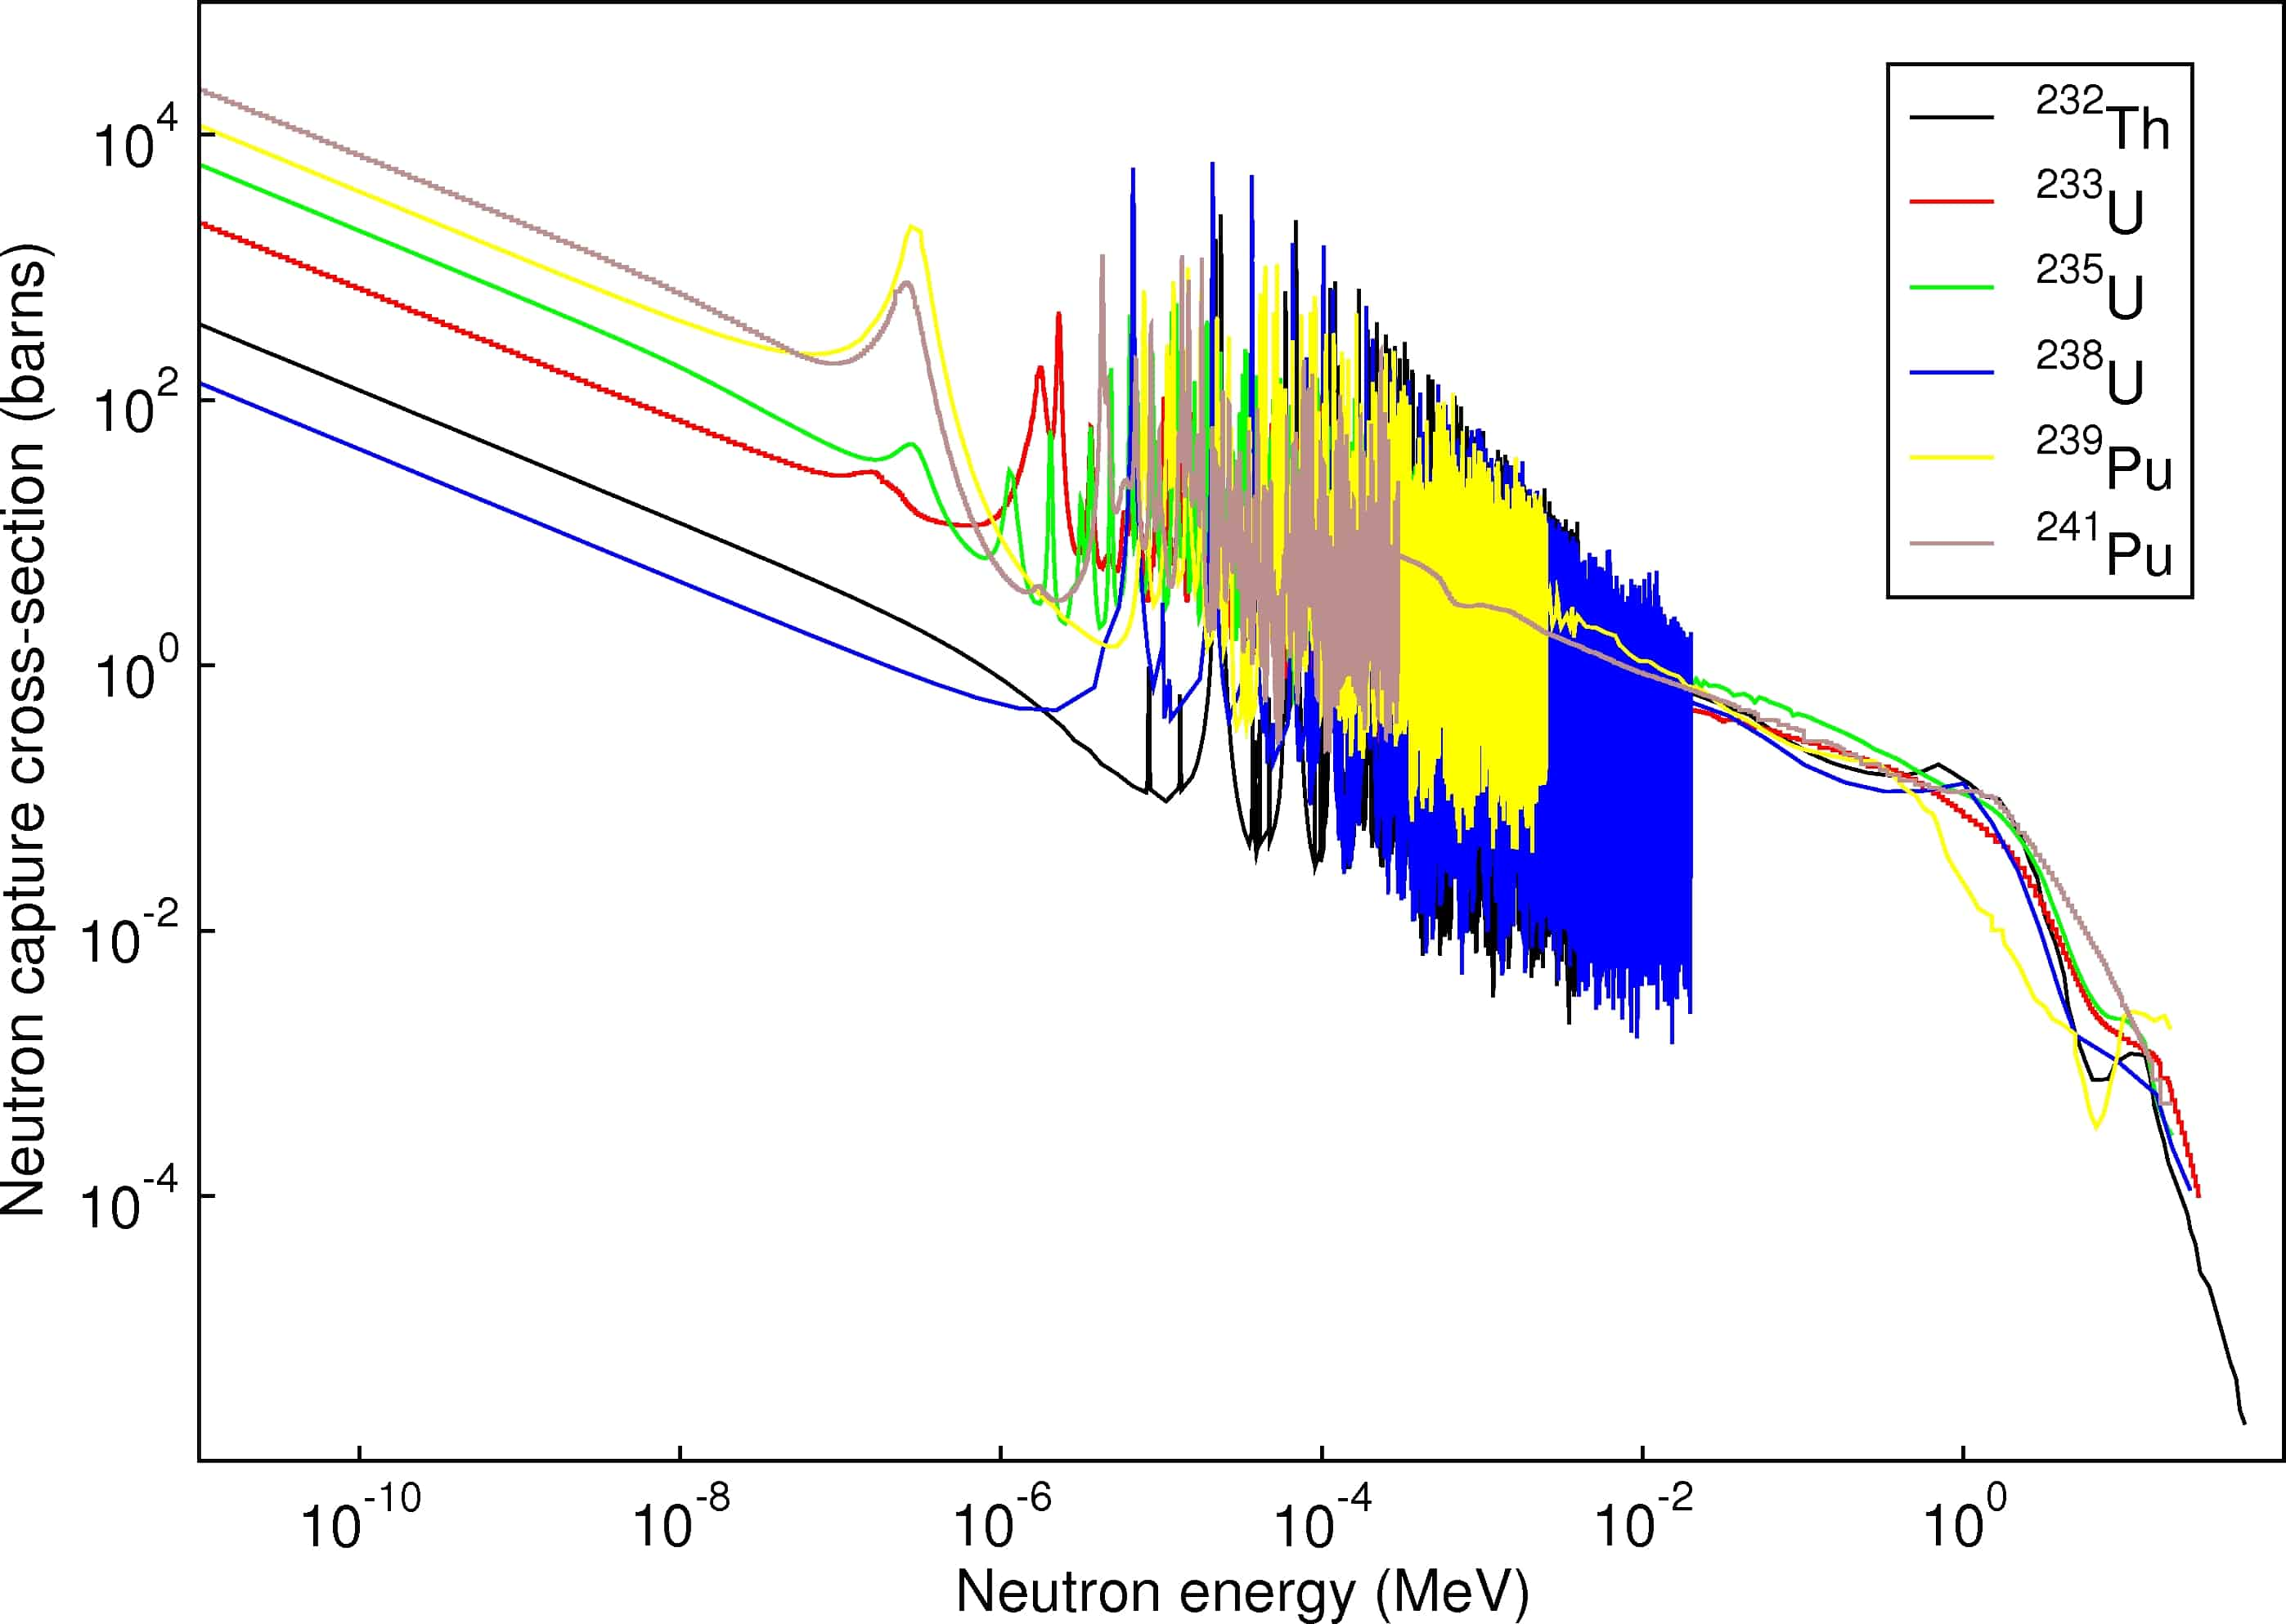
\includegraphics[width=0.75\textwidth]{fission-cs.jpg}
	\caption{Neutron-induced fission cross-section.}
	\label{fission-cs}
\end{figure}
\begin{figure}
	\centering
	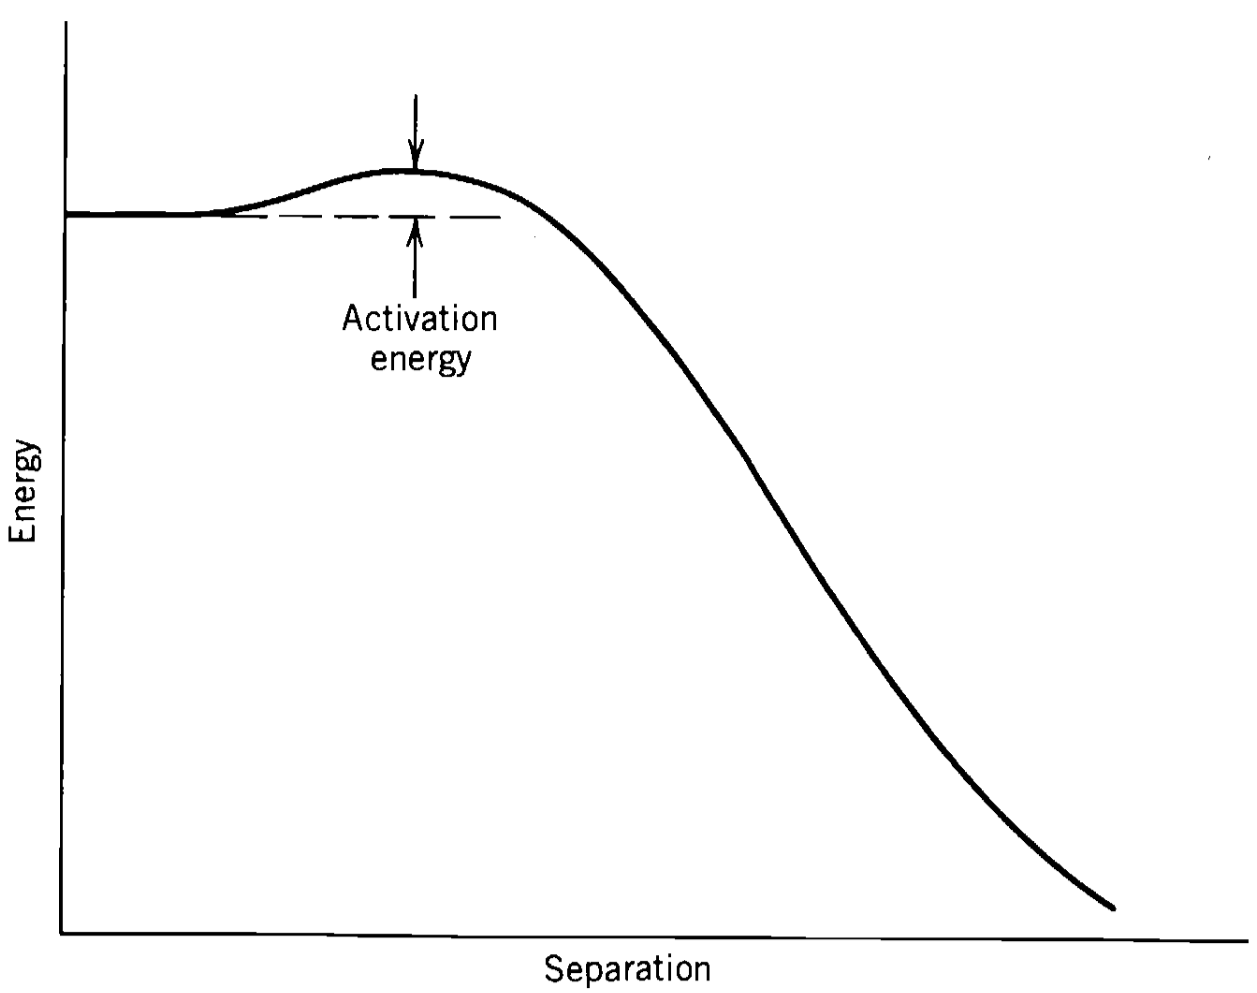
\includegraphics[width=0.75\textwidth]{fission-pot.png}
	\caption{Coulomb potential in a fissioning nucleus.}
	\label{fission-pot}
\end{figure}

\subsection{Fissione spontanea}

La tendenza dei nuclei pesanti a fissionare è evidente dall'andamento della binding energy rispetto ad $ A $ (Fig. \ref{bind-en}): ad esempio, se si considera la fissione dell'uranio $ \ch{^{235}_{92} U} \rightarrow \ch{^{90}_{36} Kr} + \ch{^{142}_{56} Ba} + 3 n $, il $ Q $-value della reazione è $ 166.73\mev $, dunque è una reazione energeticamente fortemente favorita. Va però notato che il decay branch per decadimento $ \alpha $ è fortemente dominante in natura, basta confrontare, ad esempio, i seguenti decadimenti:
\begin{equation*}
	\begin{split}
		\ch{^{238}_{92} U} \xrightarrow{4\,\text{Gy}} \ch{^{234}_{90} Th} + \alpha &\qquad \ch{^{238}_{92} U} \xrightarrow{\sim 10^7\,\text{Gy}} \ch{^{140}_{54} Xe} + \ch{^{96}_{38} Sr} + 2n\\
		\ch{^{235}_{92} U} \xrightarrow{0.7\,\text{Gy}} \ch{^{231}_{90} Th} + \alpha &\qquad \ch{^{235}_{92} U} \xrightarrow{\sim 10^8\,\text{Gy}} \ch{^{142}_{56} Ba} + \ch{^{90}_{36} Kr} + 3n
	\end{split}
\end{equation*}
La fissione è osservata solo in nuclei pesanti (il nuclide fissile più leggero è $ \ch{^{226}_{88} Ra} $), e la fissione spontanea diventa il decay mode dominante solo in nuclidi con $ A \ge 250 $.\\
Ciò che inibisce la fissione è una barriera coulombiana analoga a quella del decadimento $ \alpha $: in questo caso, però, essa ha un andamento liscio (in senso analitico), com'è possibile vedere in Fig. \ref{fission-pot}. L'energia necessaria affinché i due prodotti della fissione (supposti preformati) oltrepassino la barriera coulombiana è, nella maggior parte dei casi, troppo alta per rendere la fissione un decay mode significativo; a livello teorico, dovrebbero esistere anche dei nuclidi in cui la barriera si annulla, ovvero in cui i due prodotti hanno sempre l'energia necessaria per superarla, e tali nuclidi dovrebbero fissionare istantaneamente: naturalmente essi non esistono in natura, e si dovrebbero trovare attorno ad $ A = 300 $.\\
L'altezza della barriera coulombiana rispetto all'energia del ground state è detta activation energy ed è possibile calcolarla sia assumendo il modello semplificato a goccia sia tenendo conto degli effetti delle shell nucleari: entrambi i casi sono pllottati in Fig. \ref{act-en}.

\begin{figure}
	\centering
	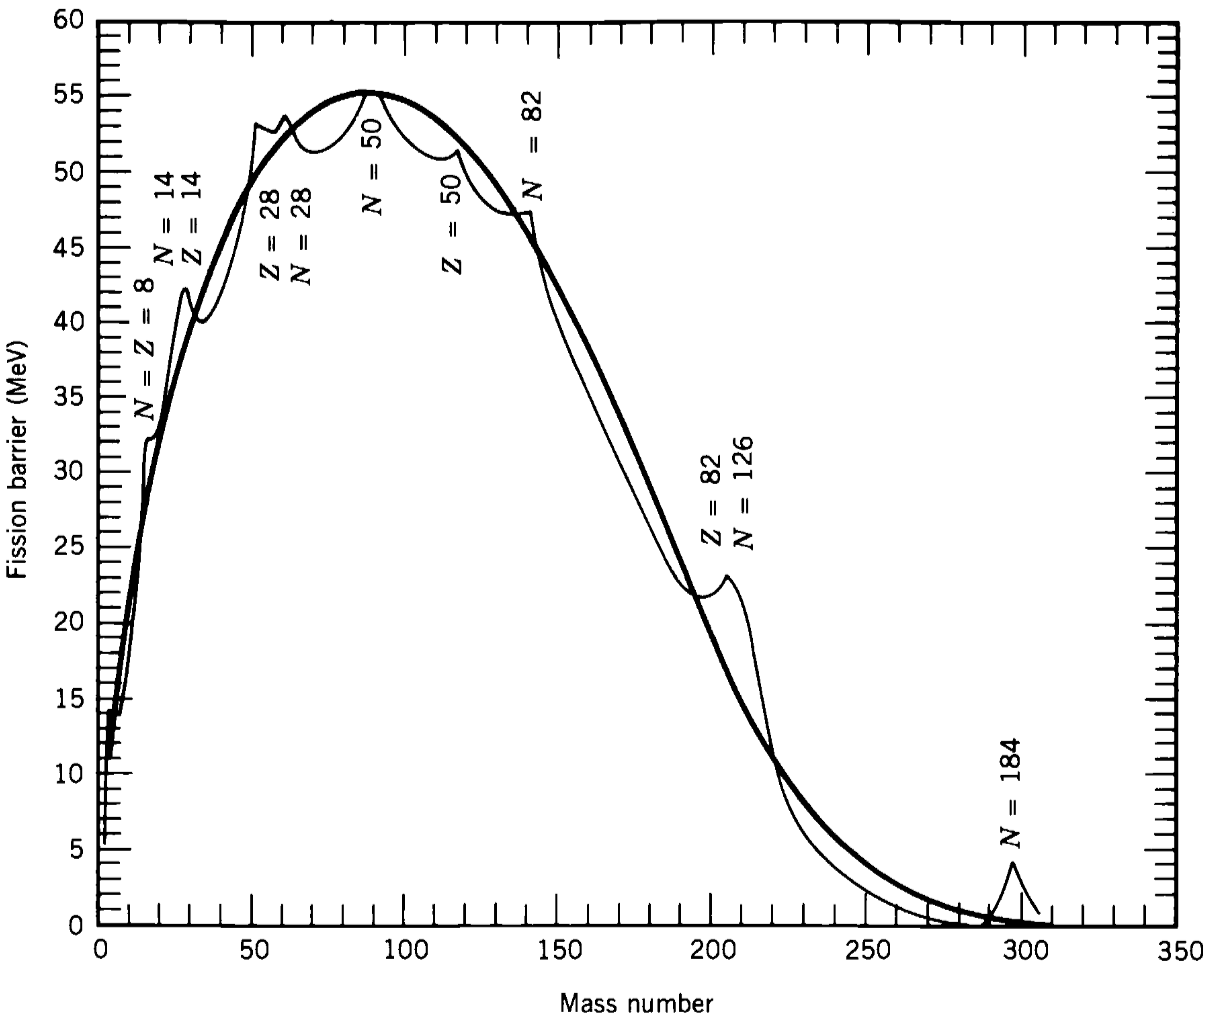
\includegraphics[width=0.65\textwidth]{act-en.png}
	\caption{Activation energy of nuclear fission.}
	\label{act-en}
\end{figure}
\begin{figure}
	\centering
	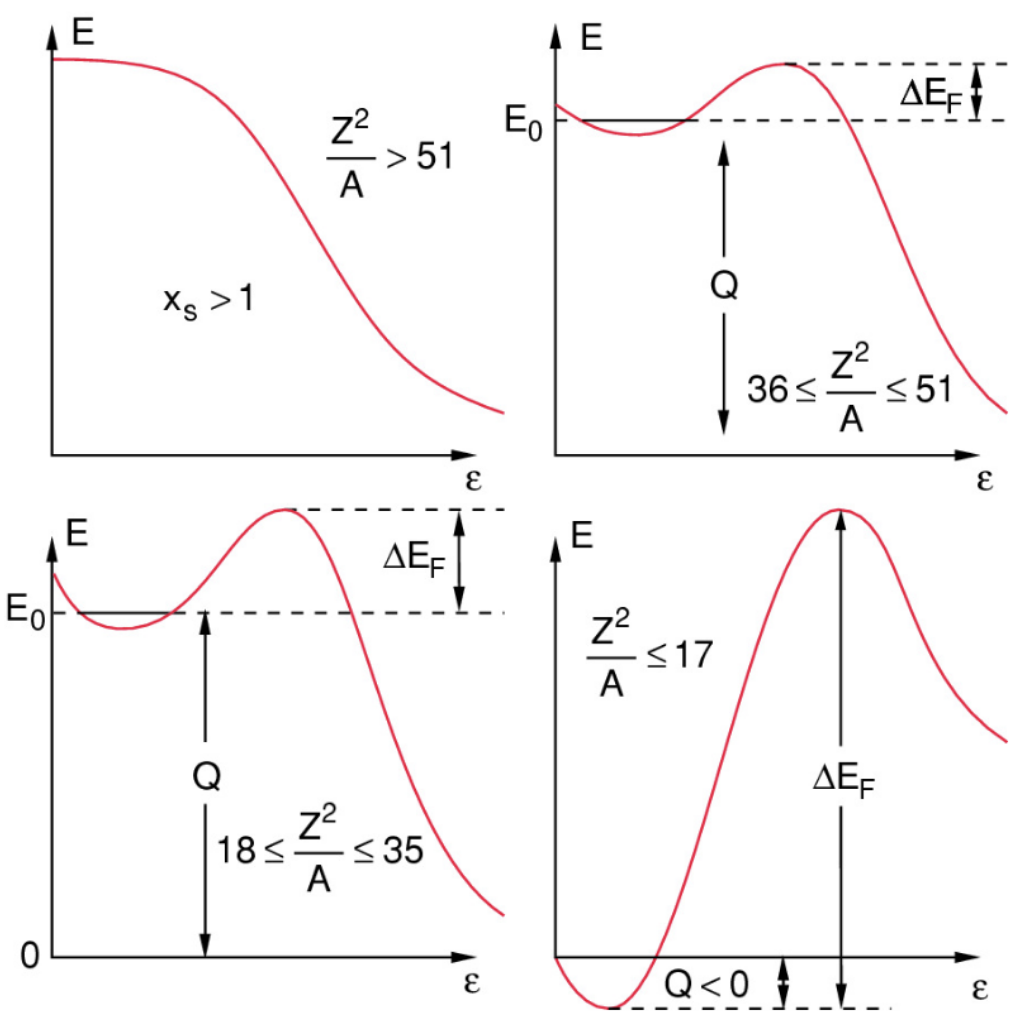
\includegraphics[width=0.60\textwidth]{act-en-z.png}
	\caption{Potential barrier as a funzion of the deformation parameter for various fissility values.}
	\label{act-en-z}
\end{figure}

\paragraph{Liquid drop model}

Semplificando, questo modello considera solo le proprietà nucleari medie, assumendo un nuclide sferico nel suo ground state. Nel caso di un nucleo fissile, l'instabilità porta ad una deformazione del nuclide in un ellissoide: assumendo il raggio iniziale $ R $ e l'eccentricità dell'ellissoide $ \varepsilon $, si possono calcolare i semiassi come:
\begin{equation}
	a = R \left( 1 + \varepsilon \right) \qquad b = R \left( 1 + \varepsilon \right)^{-1/2}
	\label{eq:2.18}
\end{equation}
Si vede dunque che il volume $ V = \frac{4}{3}\pi R^3 = \frac{4}{3} \pi ab^2 $ rimane inalterato, mentre la superficie varia di un fattore approssimabile ad $ \varepsilon $: $ S = 4\pi R^2 \left( 1 + \frac{2}{5} \varepsilon^2 + \dots \right) $; analogamente, si mostra che l'energia d'interazione coulombiana varia di un fattore $ \left( 1 - \frac{1}{5} \varepsilon^2 + \dots \right) $.\\
Dalla formula semi-empirica di Weizsäcker (Eq. \ref{eq:1.30}) deriva che, a seguito della deformazione, la binding energy varia di:
\begin{equation}
	\Delta B = - a_S A^{2/3} \left( 1 + \frac{2}{5} \varepsilon^2 + \dots \right) - a_C \frac{Z^2}{A^{1/3}} \left( 1 - \frac{1}{5} \varepsilon^2 + \dots \right) \approx \left( -\frac{2}{5} a_S A^{2/3} + \frac{1}{5} a_C \frac{Z^2}{A^{1/3}} \right) \varepsilon^2
	\label{eq:2.19}
\end{equation}
Se $ \Delta B > 0 $, il nucleo risulta instabile rispetto alla deformazione e fissiona, dunque si trova una condizione per la fissione spontanea:
\begin{equation}
	\Chi \defeq \frac{a_C}{2a_S} \frac{Z^2}{A} > 1
	\label{eq:2.20}
\end{equation}
dove è stata definita la fissility $ \Chi $. Utilizzando i valori di $ a_S $ ed $ a_C $ interpolati si trova la condizione $ Z^2 / A > 51 $, ovvero $ Z > 114 $ e $ A > 270 $; al di sotto di questi valori la fissione è possibile solo fornendo la necessaria energia di attivazione (vedere Fig. \ref{act-en-z}).\\
Bisogna specificare che per $ Z^2 / A > 51 $ la fissione spontanea è istantanea, mentre per nuclidi con $ Z^2 / A \lesssim 51 $ è possibile anche una delayed fission per effetto tunnel (a causa della repulsione tra protoni), analogamente al decadimento $ \alpha $, ma nella maggior parte dei casi quest'ultimo è dominante.
Infine, si può notare in Fig. \ref{fission-lt} come i tempi di decadimento aumentino al diminuire di $ Z^2 / A $.

\begin{figure}[!hb]
	\centering
	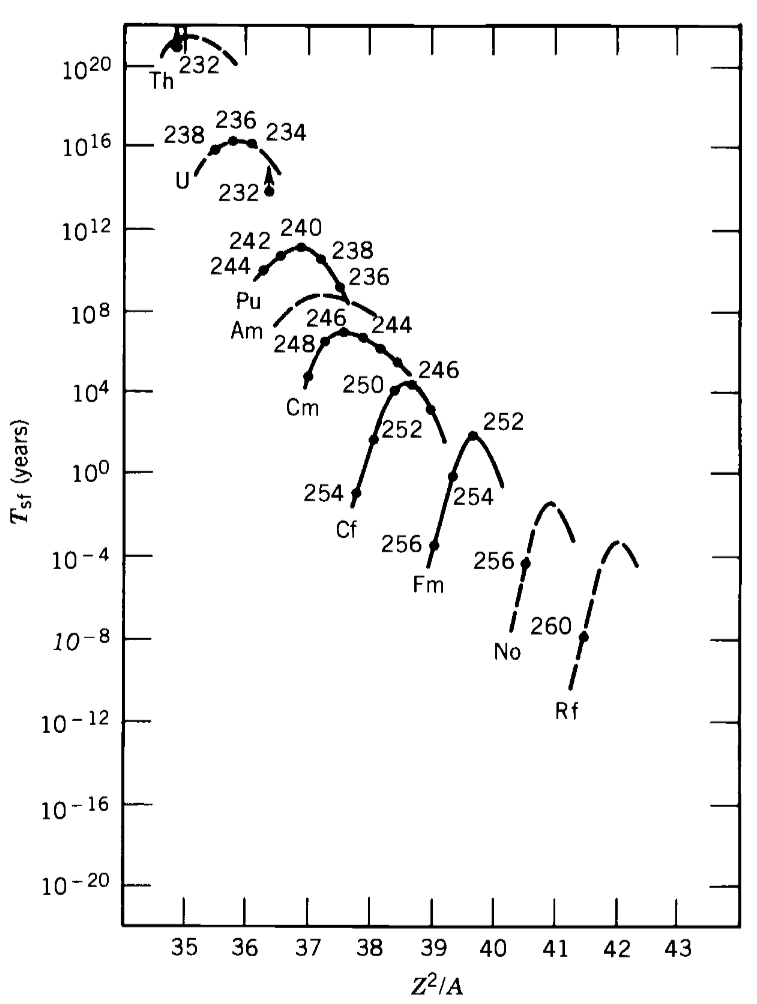
\includegraphics[width=0.80\textwidth]{fission-lt.png}
	\caption{Lifetimes for spontaneous fission.}
	\label{fission-lt}
\end{figure}

\subsection{Fissione indotta}

Dato che i neutroni non sono affetti dal potenziale coulombiano, è possibile indurre la fissione di un nuclide facendolo scatterare con un neutrone termico. Bisogna però notare una differenza tra la fissione di nuclidi pari-pari e nuclidi pari-dispari, dovuta al termine di pairing nella formula di Weizsäcker (Eq. \ref{eq:1.30}).\\
Si considerino ad esempio due campioni di $ \ch{^{235}_{92} U} $ e $ \ch{^{235}_{92} U} $ e li si irraggi con neutroni termici:
\begin{enumerate}
	\item $ \ch{^{235}_{92} U} + n \rightarrow \ch{^{236}_{92} U}^* $: $ Q = 6.5\mev > \Delta E_F = 6.1\mev $;
	\item $ \ch{^{238}_{92} U} + n \rightarrow \ch{^{239}_{92} U}^* $: $ Q = 4.8\mev < \Delta E_F = 6.4\mev $;
\end{enumerate}
Si vede dunque che la fissione di $ \ch{^{235}_{92} U} $ può avvenire con neutroni termici, mentre per quella di $ \ch{^{238}_{92} U} $ sono necessari neutroni veloci. Ciò è dovuto al fatto che i nuclidi pari-pari sono energeticamente favoriti, dunque il termine di pairing favorisce processi da pari-dispari a pari-pari, mentre ostacola quelli da pari-pari a pari-dispari: nel caso considerato, infatti, la differenza di energia ammonta a $ \Delta E = \delta (236^{-1/2} + 238^{-1/2}) = 1.5\mev $.\\
È interessante notare che $ \ch{^{235}_{92} U} $ e $ \ch{^{238}_{92} U} $ sono gli unici isotopi dell'uranio rimasti in natura, con abbondanze isotopiche rispettivamente del $ 0.72\% $ e $ 99.28\% $.

\subsection{Caratteristiche}

Il processo di fissione del nuclide non presenza grosse differenze tra il caso spontaneo e quello indotto: in maniera quasi istantanea ($ \sim 10^{-17}\,\text{s} $) il nucleo si deforma radicalmente andando a formare i due frammenti di fissione (sono possibili fissioni ternarie ma sono estremamente rare), i quali si separano in tempi brevissimi ($ \sim 10^{-14}\,\text{s} $): questi sono nuclidi molto neutron-rich, dunque espellono i neutroni con energie di legame superiori all'energia di legame media, andando così a formare i prodotti di fissione; quest'ultimi possono decadere tramite decadimenti $ \beta $ e $ \gamma $, con tempi su una scala dai secondi ai milioni di anni, muovendosi verso la valle di stabilità.

\subsubsection{Asimmetria di fissione}

I due frammenti altamente eccitati in cui si separa il nucleo a seguito della fissione non sono uguali, ma presentano una notevole asimmetria; per di più, variando il nuclide fissile si osserva che la distribuzione dei frammenti pesanti rimane praticamente inalterata, mentre la massa in eccesso viene inglobata dai frammenti leggeri (vedere Fig. \ref{fission-md}).\\
Ciò può essere spiegato dal fatto che la fissione, sebbene trattata in maniera elementare utilizzando il liquid drop model, risente in realtà degli effetti delle shell nucleari: come si può notare in Fig. \ref{fission-asimm}, la distribuzione dei frammenti pesanti si sovrappone ad una regione di completamento di shell nucleari, con la presenza anche del nuclide doubly-magic $ \ch{^{132}_{50} Sn_{82}} $, che ha una configurazione estremamente stabile; tutto ciò non accade, invece, per la distribuzione dei frammenti leggeri, i quali non si sovrappongono a nessun magic nucleus.\\
Circa metà dei prodotti di fissione decadono in meno di un anno, mentre i restanti possono avere tempi di decadimento anche di milioni di anni: questi formano le scorie radioattive.\\
I prodotti di fissione sono molto neutron-rich, dunque per la maggior parte sono instabili per decadimento $ \beta^- $: la fissione nucleare è un importante strumento di ricerca per la regione $ \beta^- $-instabile, difficilmente raggiungibile con altri metodi: i prodotti di fissione possono dar luogo ad intere catene di decadimenti $ \beta^- $.

\begin{figure}
	\centering
	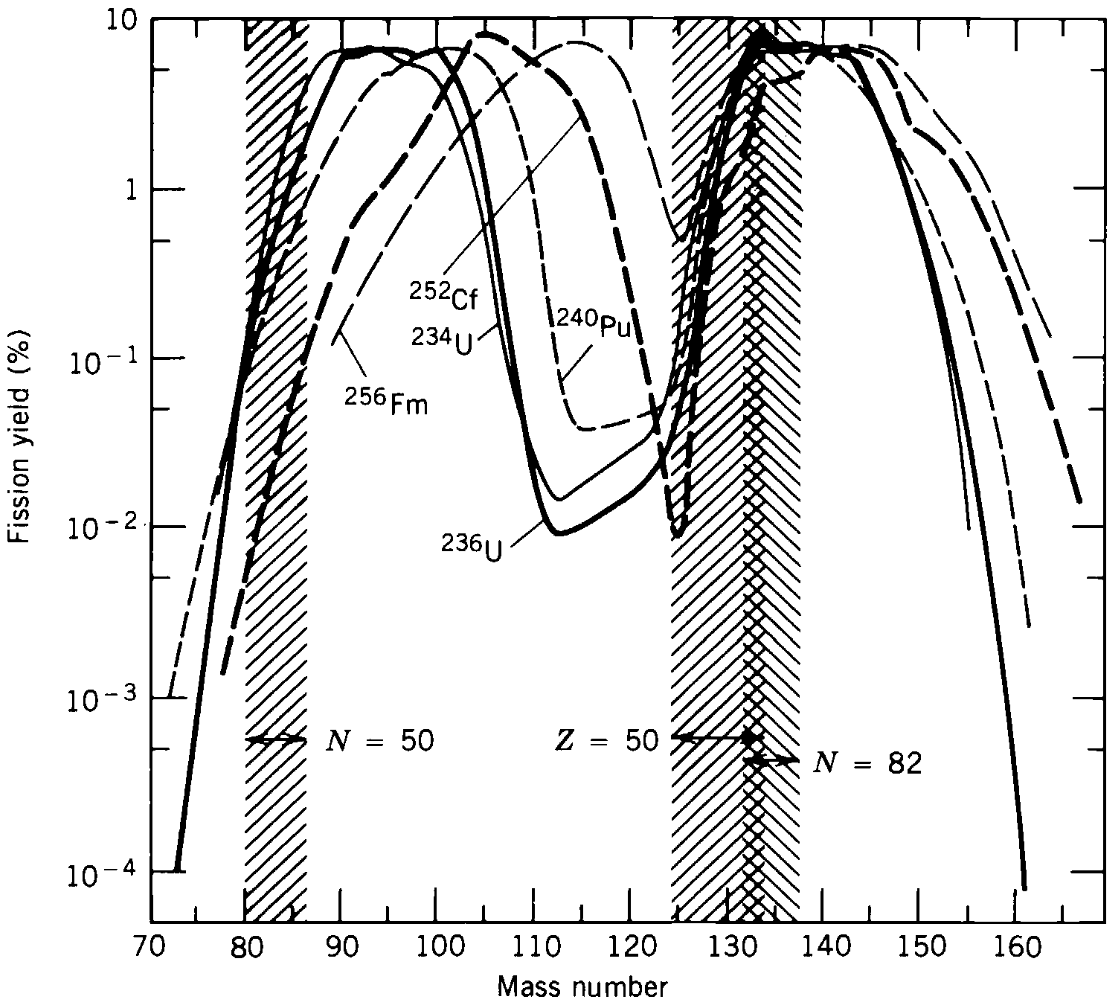
\includegraphics[width=0.60\textwidth]{fission-asimm.png}
	\caption{Asimmetry in fission products.}
	\label{fission-asimm}
\end{figure}
\begin{figure}
	\centering
	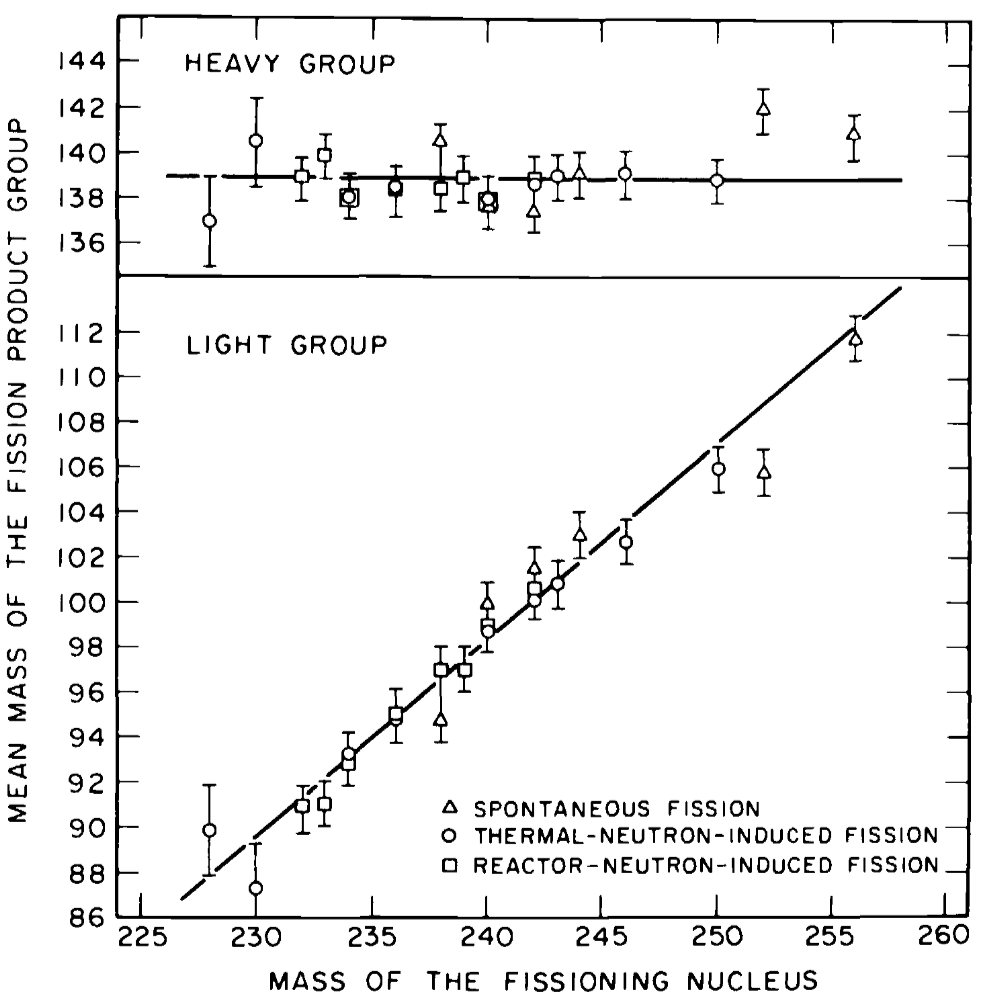
\includegraphics[width=0.60\textwidth]{fission-md.png}
	\caption{Distributions of light and heavy fission products.}
	\label{fission-md}
\end{figure}

\subsubsection{Emissione di neutroni}

I neutroni prodotti dalla fissione di un nuclide si possono distinguere in due categorie: prompt neutrons and delayed neutrons.\\
I prompt neutrons vengono emessi praticamente in contemporanea al processo di fissione, venendo emessi dal nuclide fissile e dai frammenti di fissione: il numero di prompt neutrons viene indicato come $ \nu_n $ e generalmente si ha $ \langle \nu_n \rangle \approx 2.4 $.\\
La distribuzione di prompt neutrons in base alla loro energia cinetica è una distribuzione di Maxwell, mentre $ \nu_n $ si distribuisce secondo una gaussiana indipendentemente dalla fissione considerata, come visibile in Fig. \ref{n-neut-dist}: i prompt neutrons vengono prodotti con energia di circa $ 2\mev $, in media.\\
I delayed neutrons, d'altro canto, sono quelli prodotti nelle decay chains iniziate dai prodotti di fissione, solitamente tra $ 0.2\,\text{s} $ e $ 60\,\text{s} $ dopo la fissione, e costituiscono appena l'$ 1\% $ dei neutroni totali prodotti dalla fissione.

\begin{figure}[!b]
	\centering
	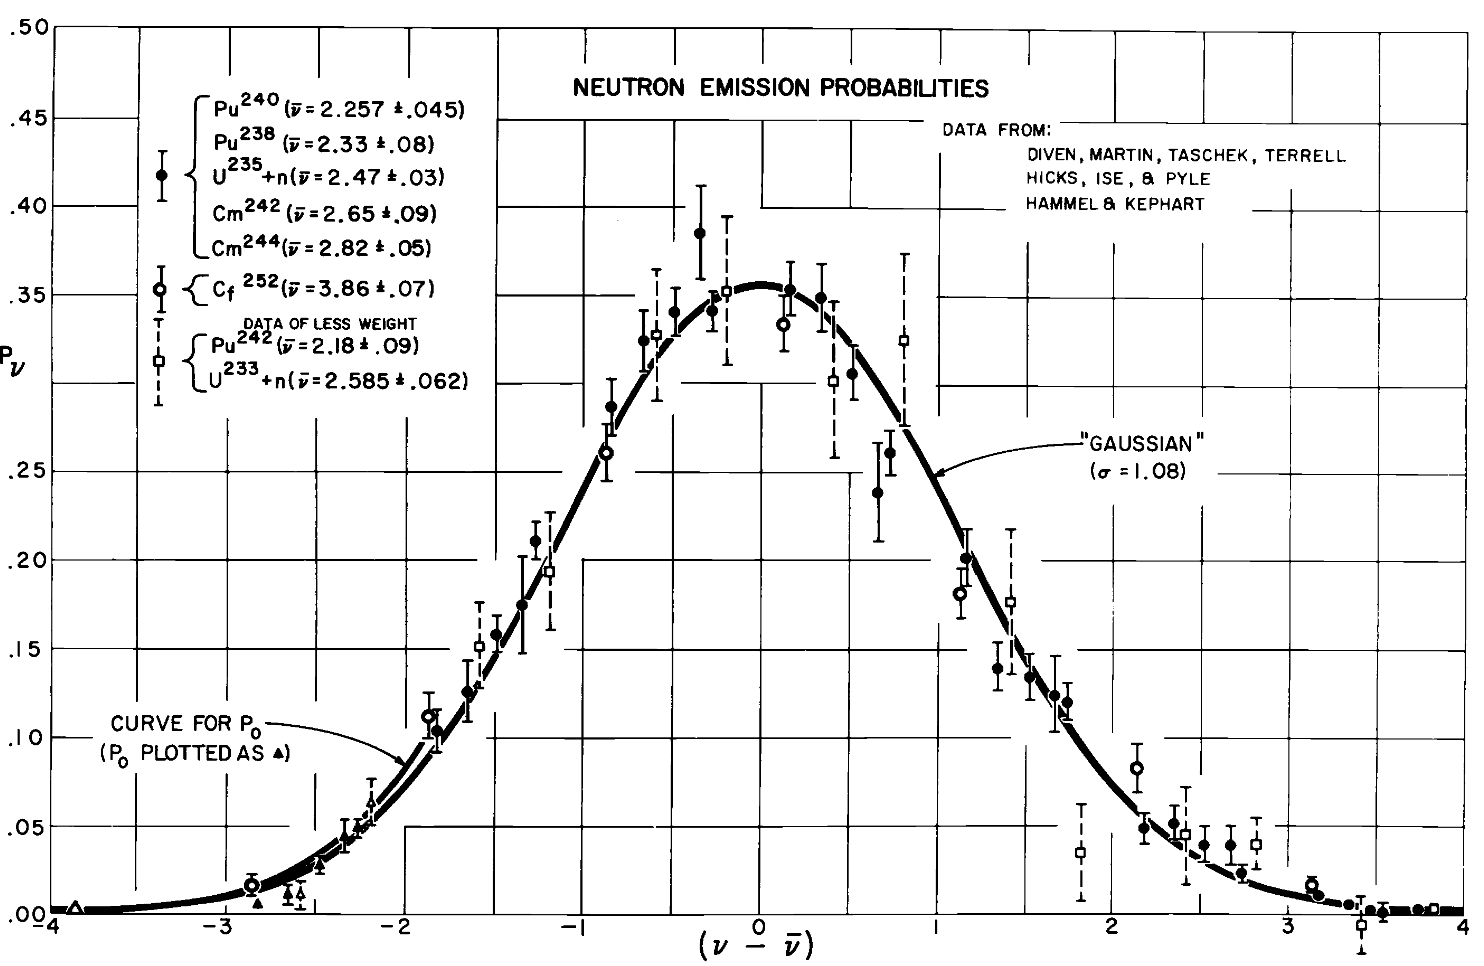
\includegraphics[width=0.75\textwidth]{n-neut-d.png}
	\caption{Prompt neutrons' number distribution.}
	\label{n-neut-dist}
\end{figure}

\subsubsection{Bilancio energetico}

Considerando, ad esempio, la fissione del $ \ch{^{235}_{92} U} $, i $ 210\mev $ di energia rilasciata vengono ripartiti nel seguente modo:
\begin{enumerate}
	\item frammenti di reazione: $ \ch{Y}_{\text{small}} \approx 100\mev $ e $ \ch{Y}_{\text{large}} \approx 70\mev $;
	\item prompt emissions: neutrons $ \approx 5\mev $ e fotoni $ \approx 7\mev $;
	\item decadimenti: $ \beta^- \approx 20\mev $ (di cui $ \approx 12\mev $ persi in neutrini) e $ \gamma \approx 8\mev $.
\end{enumerate}
La differenza tra i due frammenti è dovuta alla conservazione del momento lineare: trascurando i neutroni si ha $ m_1 \ve{v}_1 = m_2 \ve{v}_2 $, dunque $ K_1 / K_2 = m_2 / m_1 $, ovvero il frammento leggero acquista la maggior parte del'energia cinetica disponibile.

\subsection{Applicazioni}

\subsubsection{Studio della stuttura nucleare}

Dato che la fissione produce nuclidi neutron-rich eccitati molto esotici, essa può essere usata per studiare una zona difficilmente popolabile della nuclear chart, quella $ \beta^- $-instabile.\\
Inoltre, a partire dalla fissione è possibile ottenere la cosiddetta spallazione del nuclide fissile: quando il l'energia della particella proiettile è molto elevata la fissione produce frammenti multipli. Essendo il processo non più binario, la distribuzione dei frammenti non è più a doppia campana (come in Fig. \ref{fission-asimm}), ma si va a popolare anche la conca centrale: più è alta l'energia del proiettile, più saranno i frammenti di masse intermedie prodotti.\\
Questo, ad esempio, è ciò che avviene nell'esperimento ISOLDE al CERN: nuclei esotivi vengono prodotti con irraggiamento di protoni, i quali, provenendo da LHC, hanno energie dell'ordine di $ 1.5\gev $.

\subsubsection{Reattori a fissione}

Il funzionamento dei reattori a fissione nucleare si basa sulle reazioni a catena dell'uranio: queste avvengono poiché la fissione di $ \ch{^{235}_{92} U} $ produce in media 3 neutroni, i quali potenzialmente possono dar luogo ad ulteriori fissioni.\\
Il problema principale è che $ \ch{^{235}_{92} U} $ richiede un neutrone termico per fissionare, mentre i neutroni prodotti dalla fissione sono neutroni veloci: per rallentare questi neutroni, è necessario alternare nel reattore strati di materiale fissile a strati di materiale moderatore. Quest'ultimo solitamente è costituito da acqua o da grafite, materiali leggeri con una cross-section elevata per scattering neutronico (elastico) ai quali viene ceduta una grande frazione dell'energia cinetica.\\
È inoltre necessaria, come materiale fissile, una miscela di uranio con almeno il $ 3\% $ di $ \ch{^{235}_{92} U} $: per fare ciò, è necessario arricchire l'uranio estratto in natura. Il $ \ch{^{238}_{92} U} $ non è inerte, ma può fissionare quando dei neutroni veloci sfuggono alle barre di moderazione.\\
Per mantenere la reazione sotto controllo bisogna avere il giusto numero di neutroni: se non vengono prodotti abbastanza neutroni dalle fissioni la catena non riesce ad autosostenersi, mentre se ne vengono prodotti troppi c'è il rischio che essa non sia più controllabile ed esploda esponenzialmente. In particolare, data una certa massa di materiale fissile, si definisce il neutron reproduction factor $ k $ come il rapporto tra i numeri di neutroni fissili (quelli che effettivamente danno luogo a fissioni) di due generazioni successive di nuclidi fissili a catena avviata: la massa si dice critica se $ k = 1 $, supercritica se $ k > 1 $ e subcritica se $ k < 1 $.\\
L'obbiettivo, in un reattore a fissione, è mantenere il materiale fissile in stato critico, dunque controllabile: per mantenere la catena sotto controllo si utilizzano delle barre fatte di materiale ad alto potere d'assorbimento di neutroni (ad esempio bario, boro, cadmio, indio etc.), le quali possono essere inserite all'interno del materiale fissile per bloccare totalmente o in parte la reazione.\\
Un altro parametro importante nella caratterizzazione di un reattore a fissione è il numero medio di neutroni termici fissili: infatti, non tutti i neutroni termici prodotti da fissione generano a loro volta delle fissioni, poiché subentrano processi d'assorbimento. Considerando del materiale fissile composto da $ \ch{X}_i $ specie nucleari con frazioni $ x_i $, si hanno le cross-section di fissione e di assorbimento
\begin{equation}
	\sigma_f = \sum_{i} x_i \sigma_f\left( \ch{X}_i \right) \qquad \sigma_a = \sum_{i} x_i \sigma_a\left( \ch{X}_i \right)
	\label{eq:2.21}
\end{equation}
Il numero medio di neutroni termici fissili $ \eta $ risulta essere dunque:
\begin{equation}
	\eta = \frac{\sigma_f}{\sigma_f + \sigma_a} \langle \nu_n \rangle
	\label{eq:2.22}
\end{equation}
Ad esempio, per una miscela naturale di $ \ch{^{235}_{92} U} $ al $ 0.72\% $ e $ \ch{^{238}_{92} U} $ al $ 99.28\% $, dato che $ \sigma_f(235) = 584\,\text{barn} $, $ \sigma_a(235) = 97\,\text{barn} $, $ \sigma_f(238) = 0 $ ($ \ch{^{238}_{92} U} $ non fissiona con neutroni termici) e $ \sigma_a(238) = 2.75\,\text{barn} $, si hanno $ \sigma_f = 4.20\,\text{barn} $ e $ \sigma_{a} = 3.43\,\text{barn} $, quindi $ \eta = 1.33 $.\\
Considerando invece una miscela con $ \ch{^{235}_{92} U} $ arricchito al $ 3\% $, si ottiene $ \eta = 1.84 $, che permette una maggior perdita neutronica per altri processi d'assorbimento senza entrare in regime subcritico.

\section{Decadimento \texorpdfstring{$ \beta $}{TEXT}}

Il termine \textit{decadimento $ \beta $} indica collettivamente tutte le transizioni tra isobari (stesso $ A $) mediate dall'interazione debole: questi processi tendono ad ottimizzare il rapporto $ N/Z $ dei nuclidi, percorrendo catene isobariche verso la valle di stabilità. In particolare, in questi decadimenti l'interazione debole cambia un neutrone in un protone (o viceversa), producendo una coppia leptone-antileptone o trasformando un elettrone in un neutrino.\\
Si distinguono tre decadimenti separati:
\begin{enumerate}
	\item decadimento $ \beta^- $: $ n \rightarrow p^+ + e^- + \bar{\nu}_e $;
	\item decadimento $ \beta^+ $: $ p^+ \rightarrow n + e^+ + \nu_e $;
	\item electron capture: $ p + e^- \rightarrow n + \nu_e $.
\end{enumerate}
Nel caso dell'electron capture avviene che un elettrone delle shell più interne (tipicamente la shell K), il quale ha un alta probabilità di trovarsi all'interno del nucleo, venga catturato da quest'ultimo, lasciando un buco nella shell che viene subito colmato da una transizione a catena degli elettroni dell'atomo, emettendo dei raggi X caratteristici.

\subsection{Decadimento dei nucleoni}

Il decadimento $ \beta^+ $ del protone e quello $ \beta^- $ del neutrone possono essere spiegati tramite il modello a quark dei nucleoni.\\
Il protone è formato da due quark up ed un quark down: nel caso in cui esso sia parte di un nucleo può accadere che, tramite interazione debole, un quark up diventi un quark down, come mostrato nel seguente diagramma di Feynman:

\begin{figure}[h!]
	\centering
\begin{tikzpicture}
	\begin{feynman}
		\vertex (a1) {\(u\)};
		\vertex[right=4cm of a1] (ai);
		\vertex[right=4cm of ai] (a2) {\(d\)};

		\vertex[below=2em of a1] (b1) {\(u\)};
		\vertex[below=2em of b1] (c1) {\(d\)};
		\vertex[below=2em of a2] (b2) {\(u\)};
		\vertex[below=2em of b2] (c2) {\(d\)};

		\vertex[above=1.5cm of a2] (d1) {\(\nu_e\)};
		\vertex[above=3em of d1] (d2) {\(e^+\)};
		\vertex at ($(d1)!0.5!(d2) - (2cm, 0)$) (d3);

		\diagram* {
			{[edges=fermion]
				(a1) -- (ai) -- (a2),
				(b1) -- (b2),
				(c1) -- (c2),
			},
			(d2) -- [fermion, out=180, in=45] (d3) -- [fermion, out=-45, in=180] (d1),
			(ai) -- [scalar, bend left, edge label=\(W^+\)] (d3),
		};

		\draw [decoration={brace}, decorate] (c1.south west) -- (a1.north west)
			node [pos=0.5, left] {\(p^+\)};
		\draw [decoration={brace}, decorate] (a2.north east) -- (c2.south east)
			node [pos=0.5, right] {\(\,n\)};
	\end{feynman}
\end{tikzpicture}
\end{figure}

Al contrario dei protoni confinati nei nuclei, si pensa che i protoni liberi siano stabili: se decadessero, gli esperimenti fissano un limite inferiore alla vita media $ \tau_p > 1.6 \cdot 10^{33} \,\text{y} $; ciò è comprensibile ricordando che $ m_n = 939.565 \mev/c^2 > m_p = 938.272 \mev/c^2 $.\\
Per quanto riguarda invece il neutrone, composto da un quark up e due quark down, il decadimento è analogo:

\begin{figure}[h!]
	\centering
\begin{tikzpicture}
	\begin{feynman}
		\vertex (a1) {\(d\)};
		\vertex[right=4cm of a1] (ai);
		\vertex[right=4cm of ai] (a2) {\(u\)};

		\vertex[below=2em of a1] (b1) {\(u\)};
		\vertex[below=2em of b1] (c1) {\(d\)};
		\vertex[below=2em of a2] (b2) {\(u\)};
		\vertex[below=2em of b2] (c2) {\(d\)};

		\vertex[above=1.5cm of a2] (d1) {\(\bar{\nu}_e\)};
		\vertex[above=3em of d1] (d2) {\(e^-\)};
		\vertex at ($(d1)!0.5!(d2) - (2cm, 0)$) (d3);

		\diagram* {
			{[edges=fermion]
				(a1) -- (ai) -- (a2),
				(b1) -- (b2),
				(c1) -- (c2),
			},
			(d1) -- [fermion, out=180, in=-45] (d3) -- [fermion, out=45, in=180] (d2),
			(ai) -- [scalar, bend left, edge label=\(W^-\)] (d3),
		};

		\draw [decoration={brace}, decorate] (c1.south west) -- (a1.north west)
			node [pos=0.5, left] {\(n\)};
		\draw [decoration={brace}, decorate] (a2.north east) -- (c2.south east)
			node [pos=0.5, right] {\(\,p^+\)};
	\end{feynman}
\end{tikzpicture}
\end{figure}

I neutroni liberi sono instabili poiché $ m_n > m_p $, mentre per neutroni nei nuclei il $ Q $-value del decadimento dipende dalle energie di legame dei nuclidi.\\
Sebbene instabili, i neutroni liberi sono long-lived ($ \tau_n = 885.7 \pm 0.8 \,\text{s} \approx 14.76 \,\text{min} $), dunque possono essere usati negli esperimenti: non è ancora noto come il neutrone abbia una vita media così lunga.

\subsection{Decadimento dei nuclidi}

Per quanto riguarda i nuclidi, il decadimento $ \beta^- $ è energeticamente favorevole per i nuclidi con un eccesso neutronico, mentre quello $ \beta^+ $ lo è per i nuclidi con eccesso protonico; inoltre, la electron capture è un processo che compete col decadimento $ \beta^+ $, ma non ad esso sovrapponibile, come si evince dal blancio energetico dei decadimenti (massa dei neutrini ignorata poiché $ m_{\nu_e} < 7 \ev/c^2 $):
\begin{enumerate}
	\item decadimento $ \beta^- $: $ M(A,Z) > M(A,Z + 1) $, ovvero $ Q > 0 $;
	\item decadimento $ \beta^+ $: $ M(A,Z) > M(A,Z - 1) + 2 m_e c^2 $, ovvero $ Q > 1.02\mev $;
	\item electron capture (EC): $ M(A,Z) > M(A,Z - 1) + \varepsilon $, ovvero $ Q > \varepsilon $.
\end{enumerate}
Si noti che il bilancio del decadimento $ \beta^- $ non deve tener conto dell'elettrone prodotto, dato che esso è considerato in $ M(A,Z + 1) $, mentre quello del decadimento $ \beta^+ $ deve considerare sia il positrone che l'elettrone in più nel nuclide figlio; inoltre, nell'EC si deve considerare il buco lasciato nella shell elettronica K, che porta ad un'energia d'eccitazione $ \varepsilon $.\\
Si vede immediatamente che l'EC ha $ 2 m_e c^2 - \varepsilon $ energia disponibile in più, quindi ci possono essere casi in cui il decadimento $ \beta^+ $ non può accadere ma l'ER sì.\\
Essendo il decadimento $ \beta $ un processo isobarico, bisogna ricordare che la formula di Weizsäcker per $ A $ costante è una parabola, dunque presenterà un minimo (nella valle di stabilità), ed inoltre il termine di pairing impone una trattazione separata dei nuclei con $ A $ pari e di quelli con $ A $ dispari (vedere Fig. \ref{iso-chain}).

\subsubsection{Nuclidi con \texorpdfstring{$ A $}{TEXT} dispari}

Sempre in riferimento alla Fig. \ref{iso-chain}, è possibile vedere come agisce il decadimento $ \beta $ in catene isobariche con $ A $ dispari:
\begin{align*}
	\ch{^{101}_{42} Mo} \rightarrow \ch{^{101}_{43} Tc} + e^- + \bar{\nu}_e &\qquad\qquad\qquad \ch{^{101}_{46} Pd} \rightarrow \ch{^{101}_{45} Rh} + e^+ + \nu_e \\
	\ch{^{101}_{43} Tc} \rightarrow \ch{^{101}_{44} Ru} + e^- + \bar{\nu}_e &\qquad\qquad\qquad \ch{^{101}_{45} Rh} \rightarrow \ch{^{101}_{44} Ru} + e^+ + \nu_e
\end{align*}
$ \ch{^{101}_{44} Ru} $ è il nuclide stabile della catena isobarica $ A = 101 $.

\subsubsection{Nuclidi con \texorpdfstring{$ A $}{TEXT} pari}

A causa della doppia parabola, ogni nuclide dispari-dispari ha un nuclide pari-pari corrispondente maggiormente legato, dunque sono tutti instabili; fanno eccezzione i nuclidi leggeri $ \ch{^2 H} $, $ \ch{^6 Li} $, $ \ch{^{10} B} $ e $ \ch{^{14} N} $, per i quali la diminuzione della pairing energy è bilanciata dall'asymmetry energy.\\
In regioni di massa particolari è possibile che al posto di un decadimento $ \beta $ diretto, magari energeticamente non consentito, avvenga un doppio decadimento $ \beta $ (indicato con $ \beta\beta $); è questo il caso, ad esempio, della catena isobarica $ A = 106 $, mostrata in Fig. \ref{iso-chain}: non è possibile per il $ \ch{^{106}_{48} Cd} $ decadere nel $ \ch{^{106}_{47} Ag} $ tramite decadimento $ \beta^+ $ poiché energeticamente proibito, ma molto raramente ($ t_{1/2} = (4.4 \pm 0.6) \cdot 10^{19} \,\text{y} $) esso può decadere tramite $ \beta\beta $ direttamente nel $ \ch{^{106}_{46} Pd} $:
\begin{equation*}
	\ch{^{106}_{48} Cd} \rightarrow \ch{^{106}_{46} Pd} + 2e^+ + 2\nu_e
\end{equation*}
Sebbe estremamente raro, il decadimento $ \beta\beta $ è molto importante dal punto di vista della ricerca, poiché permette di testare la teoria di Majorana: il neutrino fu introdotto da Pauli come una particella di massa molto piccola, priva di carica e con spin $ s = \frac{1}{2} $ ad hoc per spiegare le proprietà del decadimento $ \beta $; Majorana successivamente teorizzo che se la massa del neutrino fosse precisamente nulla, allora il neutrino potrebbe essere la sua stessa antiparticella (una cosiddetta particella di Majorana). Una conseguenza della teoria di Majorana sarebbe l'esistenza di un processo ancora più raro del decadimento $ \beta\beta $, il neutrino-less double beta decay ($ 0\nu\beta\beta $), in cui i due neutrini prodotti dal doppio decadimento si annichilano: ciò evidentemente viola la conservazione del numero leptonico, mettendo in discussione l'intero modello standard. Questo decadimento non è mai stato osservato e, qualora fosse effettivamente possibile, dovrebbe essere incredibilmente raro, con limiti teorici imposti da esperimenti come CUORE@LNGS superiori all'eventuale vita media del protone ($ \tau > 3.6 \cdot 10^{24} \,\text{y} $ per il $ \ch{^{128}_{52} Te} $).

\subsection{Energy spectrum}

La necessità di introdurre una nuova particella per spiegare il decadimento $ \beta $ si capisce bene analizzando lo spettro energetico prodotto da tale processo.\\
A differenza del decadimento $ \alpha $, nel quale lo spettro presenta linee discrete di energia date dalla natura mono-energetica dei decadimenti a due corpi, gli elettroni emessi dal decadimento $ \beta $ presentano uno spettro energetico continuo: ciò sarebbe impossibile per un decadimento a due corpi, anche perché l'elettrone è 2000 volte più leggero del protone, dunque dovrebbe ricevere praticamente tutta l'energia cinetica disponibile. La conclusione è che ci deve essere una terza particella come prodotto di decadimento, appunto il neutrino elettronico, che prende parte dell'energia cinetica totale disponibile.
Un tipico spettro energetico da decadimento $ \beta $ è riportato in Fig. \ref{beta-spectrum}: si nota che la distribuzione termina quando l'energia dell'elettrone acquista il suo valore massimo $ Q - m_{\nu_e} c^2 \equiv Q_{\beta} $.\\
Un'altra differenza tra decadimento $ \alpha $ e $ \beta $ è che nel decadimento $ \alpha $ si suppone che il nucleo di $ \ch{^4 He} $ esista già all'interno del nucleo, mentre nel decadimento $ \beta $ l'elettrone viene $ \virgolette{creato} $ nel processo ed immediatamente espulso dal nucleo.

\begin{figure}[b!]
	\centering
	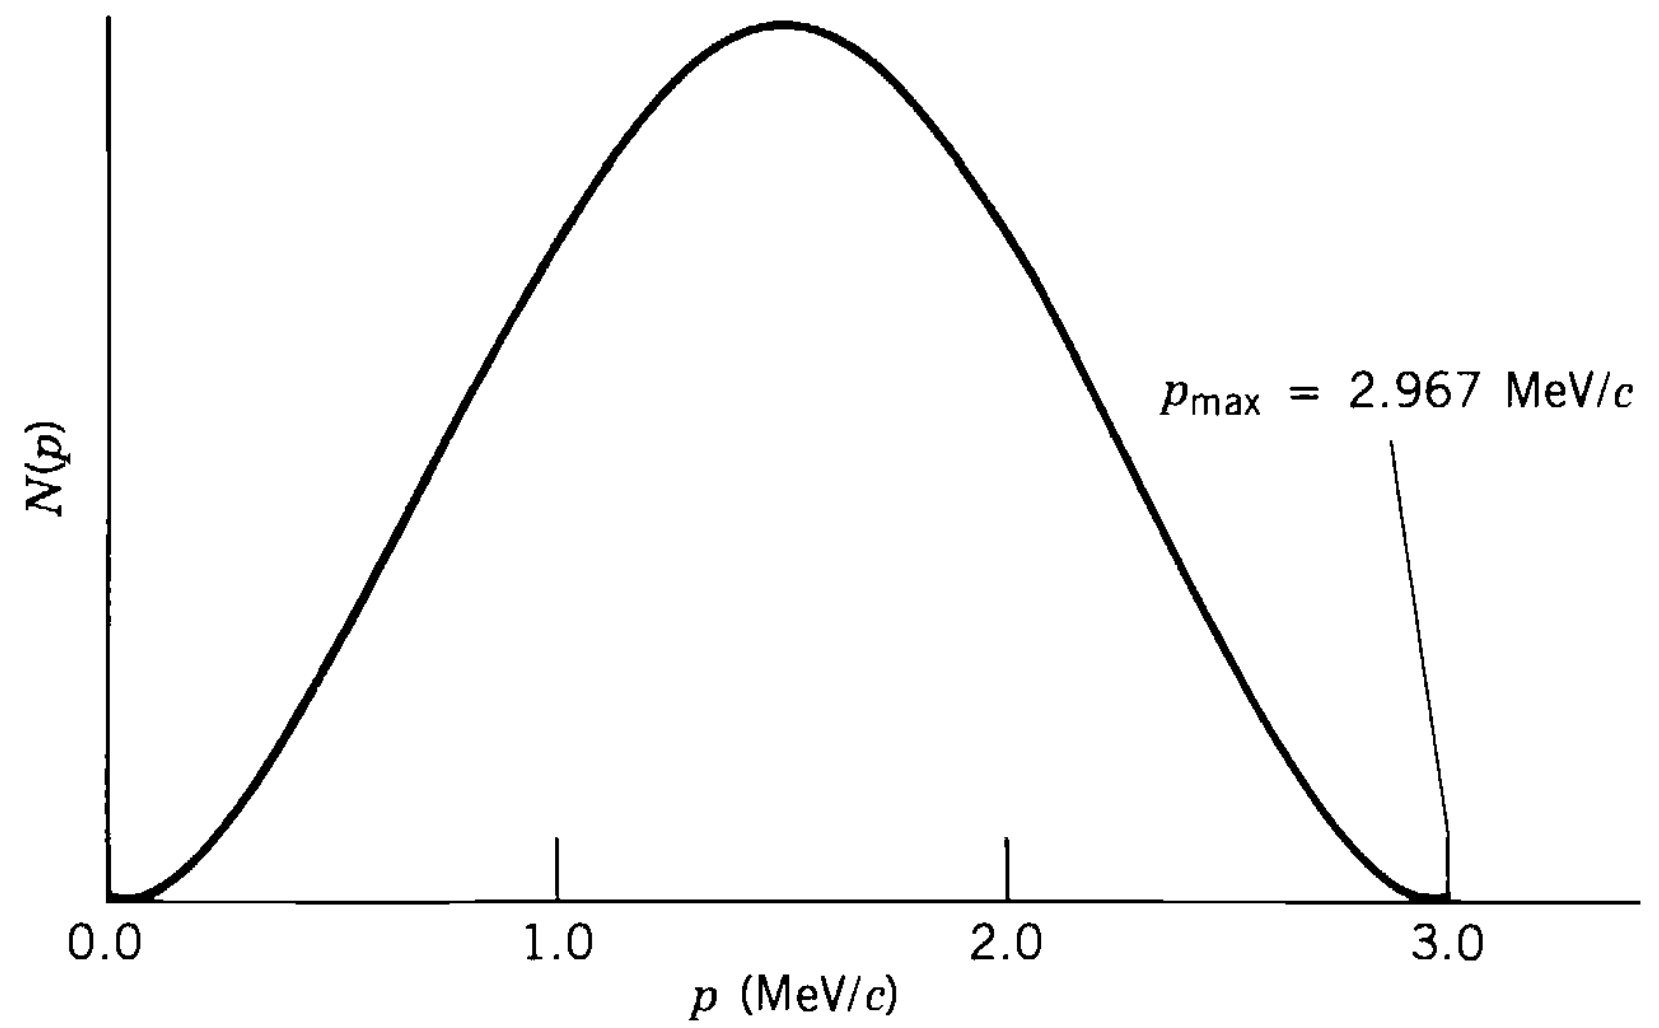
\includegraphics[width=0.45\textwidth]{beta-mom.png}
	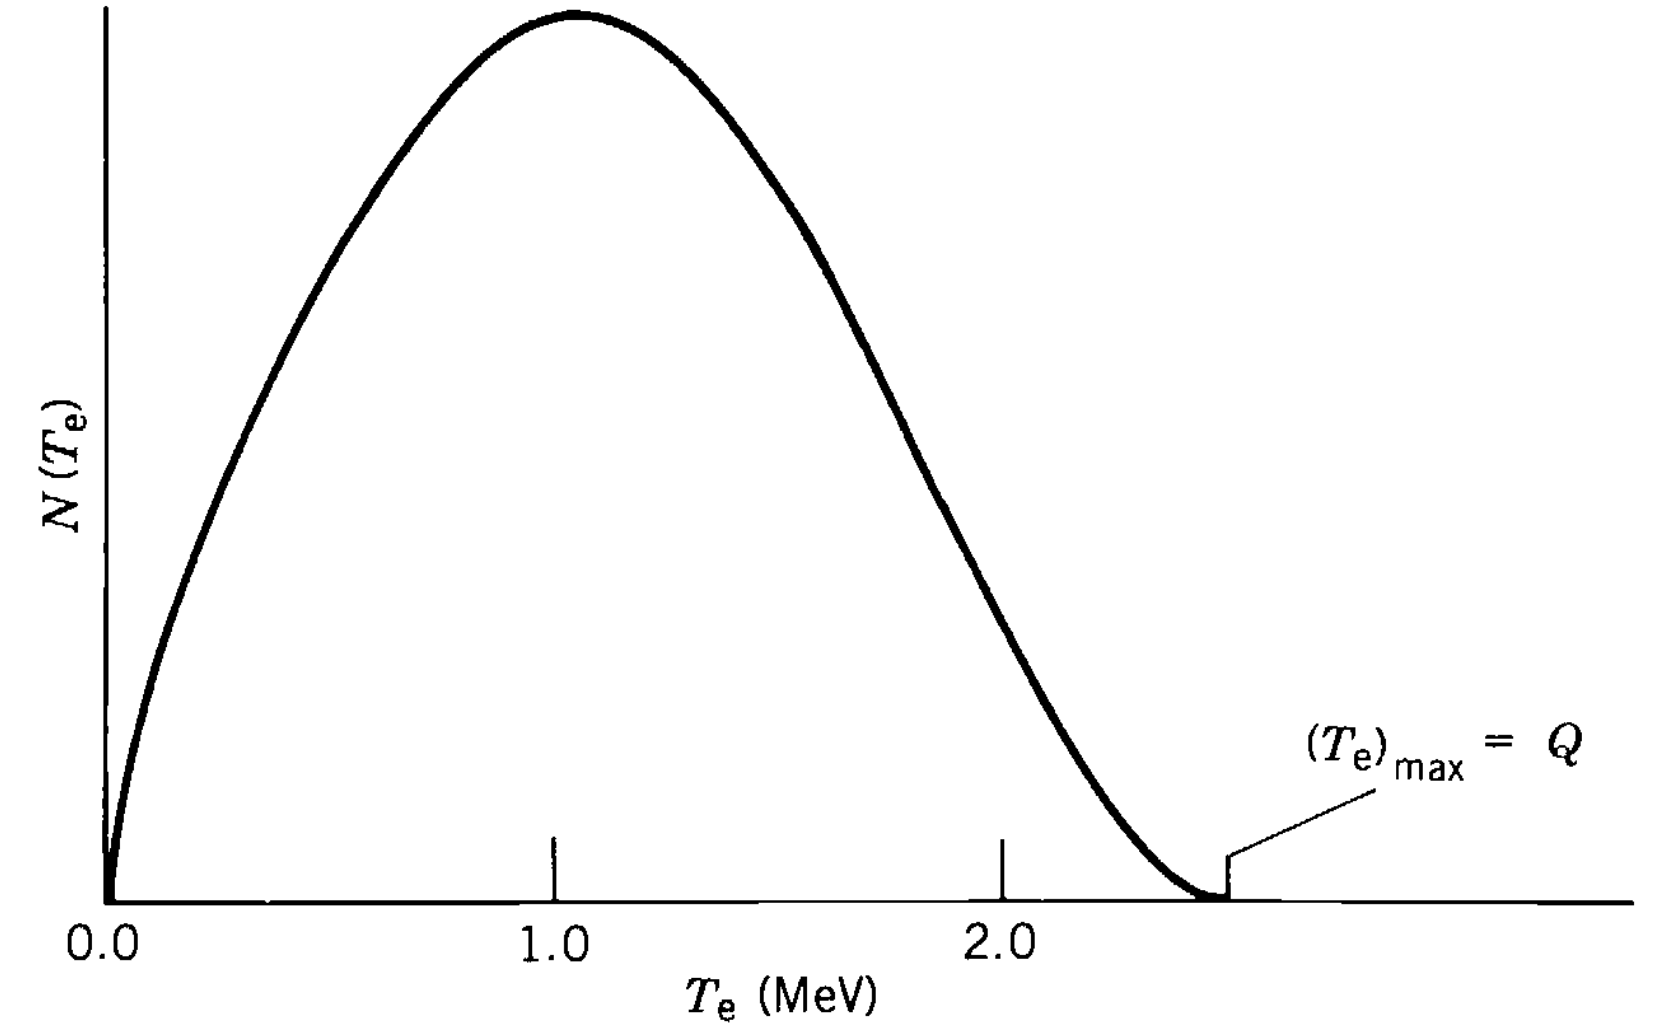
\includegraphics[width=0.45\textwidth]{beta-kin.png}
	\caption{Momentum and energy distributions of electrons from $ \beta $ decay.}
	\label{beta-spectrum}
\end{figure}

Analizzando gli spettri energetici, inoltre, si trova che $ Q_{\beta} \approx Q $: ciò implica che il neutrino ha massa estremamente piccola. Inoltre, per conservazione del momento angolare, è necessario che esso abbia spin semi-intero: considerando ad esempio il decadimento $ \ch{^{14}_6 C} \rightarrow \ch{^{14}_7 N} + e^- + \bar{\nu}_e $, se il neutrino non avesse spin semi-intero si avrebbe una violazione della conservazione di $ I $, dato che entrambi i nuclidi hanno $ I $ intero e l'elettrone ha $ s = \frac{1}{2} $.

\subsection{Teoria di Fermi}\label{fermi-th-sec}

A partire dall'ipotesi del neutrino di Pauli (1931), nel 1934 Fermi formulò una teoria per descrivere il decadimento $ \beta $; in particolare, si fanno le seguenti assunzioni:
\begin{enumerate}
	\item si trascura l'interazione coulombiana tra elettrone e nucleo (valido per nuclei con $ Z < 10 $);
	\item si trascura il nuclear recoil (valido poiché $ m_e \ll M_{\text{nucleo}} $);
	\item si considera il neutrino massless;
	\item si considerano equiprobabili tutte le possibili partizioni dell'energia tra elettrone e neutrino.
\end{enumerate}
Da questi assunti, si ricava che il bilancio energetico del processo è dato da:
\begin{equation}
	E = E_e + E_{\nu} = T_e + m_e c^2 + c p_{\nu}
	\label{eq:2.23}
\end{equation}
dalla quale si trova che $ T_e^{\text{max}} = E - m_e c^2 = Q $. La legge fondamentale postulata da Fermi per descrivere il decadimento è la \textit{golden rule}:
\begin{equation}
	\lambda = \frac{2\pi}{\hbar} \abs{M}^2 \frac{dn}{dE}
	\label{eq:2.24}
\end{equation}
Il termine $ \frac{dn}{dE} $ è dovuto alla natura dello spazio delle fasi e rappresenta la densità degli stati finali possibili per il decadimento ($ dn $ sono gli stati finali energeticamente possibili tra $ E $ ed $ E + dE $), mentre $ \abs{M}^2 $ è detto elemento di matrice dell'operatore di transizione $ \hat{H} $ e stima la probabilità di overlap tra lo stato iniziale e quello finale del sistema:
\begin{equation}
	M \defeq \braket{\psi_{\text{f}} | \hat{H} | \psi_{\text{i}}} = \int_V d^3\ve{x}\, \psi^*_{\text{f}}(\ve{x}) \hat{H} \psi_{\text{i}}(\ve{x})
	\label{eq:2.25}
\end{equation}
dove $ \psi_{\text{f}} = \psi_{\text{Y}} \psi_e \psi_{\nu} $. Il calcolo dell'elemento di matrice è estremamente complicato, specialmente per la difficoltà di calcolare le funzioni d'onda nucleari.\\
Si supponga che nel decadimento l'elettrone venga emesso con momento $ \ve{p}_e $: dato che la direzione di emssione è ininfluente con le semplificazioni fatte, ricordando che l'elemento di volume minimo dello spazio delle fasi è $ h^3 $ si trova che, confinando il sistema in un volume $ V $ (formalità solo per normalizzare le funzioni d'onda), il numero $ dn_e $ di stati elettronici finali con momento tra $ p_e $ e $ p_e + dp_e $ è:
\begin{equation}
	dn_e = \frac{4\pi p_e^2 V}{h^3} dp_e
	\label{eq:2.26}
\end{equation}
Ragionando analogamente per il neutrino, si trova che il numero totale di stati $ dn $ in funzione dei momenti $ p_e $ e $ p_{\nu} $ è:
\begin{equation}
	dn = dn_e dn_{\nu} = \left( \frac{4\pi V}{h^3} \right)^2 p_e^2 dp_e p_{\nu}^2 dp_{\nu}
	\label{eq:2.27}
\end{equation}
Ricordando il vincolo $ E = E_e + E_{\nu} $, si ha che $ cp_{\nu} = E - E_e $ e, fissata $ E_e $, $ dp_{\nu} = \frac{dE}{c} $, quindi:
\begin{equation}
	\frac{dn}{dE} = \left( \frac{4\pi V}{h^3} \right)^2 \frac{1}{c^3} (E - E_e)^2 p_e^2 dp_e
	\label{eq:2.28}
\end{equation}
Si assume $ \abs{M}^2 $ indipendente da $ p_e $, me è necessario considerare una correzione dovuta all'interazione coulombiana a cui è soggetto l'elettrone/positrone: come si vede in Fig. \ref{beta-coul}, la repulsione dei positroni porta ad averne meno ad energie basse, mentre l'attrazione degli elettroni diminuisce quelli ad alta energia. La correzione analitica è data dalla \textit{funzione di Fermi}:
\begin{equation}
	F(Z,E_e) \approx \frac{2\pi \eta}{1 - e^{-2\pi \eta}}
	\label{eq:2.29}
\end{equation}
dove $ \eta $ è il \textit{parametro di Sommerfeld}, che per $ e^{\pm} $ è definito come:
\begin{equation}
	\eta \equiv \mp \frac{Ze^2}{\hbar v_e}
	\label{eq:2.30}
\end{equation}
con $ v_e $ velocità asintotica dell'elettrone/positrone. Per $ \eta \ll 1 $ si ha $ F(Z,E_e) \approx 1 $.\\
È dunque possibile esprimere la probabilità di disintegrazione differenziale grazie alla golden rule:
\begin{equation}
	d\lambda(p_e) = C \abs{M}^2 F(Z,E_e) (E - E_e)^2 p_e^2 dp_e
	\label{eq:2.31}
\end{equation}
con $ C $ una costante. È stato possibile eliminare la dipendenza dal neutrino poiché la sua energia è fissata da quella dell'elettrone/positrone.

\begin{figure}[b!]
	\centering
	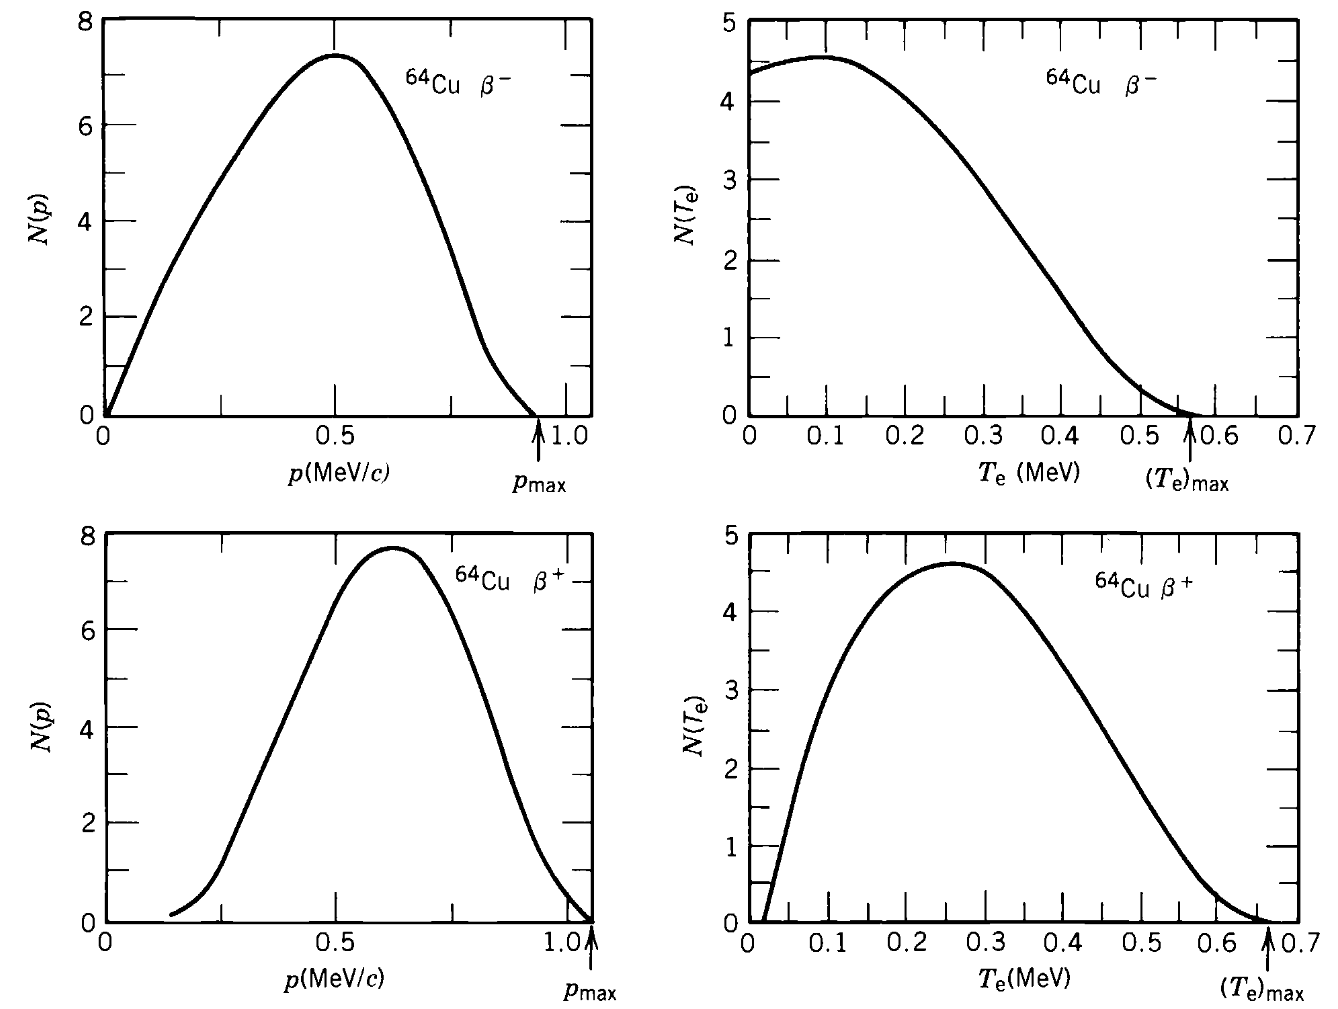
\includegraphics[width=0.70\textwidth]{beta-coul.png}
	\caption{Momentum and kinetic energy spectra of electrons and positrons emitted from $ \ch{^{64}_{29}Cu} $ decay.}
	\label{beta-coul}
\end{figure}

È possibile ottenere $ \lambda $ integrando su $ [0, p_e^{\text{max}}] $, dove il momento elettronico massimo si ottiene ponendo nullo quello neutrinico, ovvero $ p_e^{\text{max}} = \frac{1}{c} \sqrt{E^2 - m_e^2 c^4} $.\\
È inoltre utile definire la \textit{funzione di Fermi-Kurie}:
\begin{equation}
	K(E_e) \defeq \sqrt{\frac{\frac{d\lambda(p_e)}{dp_e}}{p_e^2 F(Z,E_e)}} \propto E - E_e
	\label{eq:2.32}
\end{equation}
Dall'analisi del Fermi-Kurie plot è possibile ottenere informazioni sulla massa del neutrino: infatti, con metodi di regressione lineare è possibile individuare quando $ E - E_e $ si annulla con una buona precisione, mentre misurare in maniera diretta il valore di energia massimo sarebbe complicato.

\subsubsection{Massa del neutrino}

Nel caso in cui si consideri un neutrino di massa non-nulla $ m_{\nu} $, la sua energia va calcolata come:
\begin{equation}
	E_{\nu} = \sqrt{p_{\nu}^2 c^2 + m_{\nu}^2 c^4}
	\label{eq:2.33}
\end{equation}
Differenziando $ p_{\nu}^2 c^2 = (E - E_e)^2 - m_{\nu}^2 c^4 $ e moltiplicando per $ p_{\nu} $, si trova:
\begin{equation}
	p_{\nu}^2 dp_{\nu} = \frac{1}{c^3} \sqrt{(E - E_e)^2 - m_{\nu}^2 c^4} (E - E_e) dE
	\label{eq:2.34}
\end{equation}
Dall'Eq. \ref{eq:2.27}-\ref{eq:2.31}, si trova quindi l'equazione corretta:
\begin{equation}
	d\lambda(p_e) = C \abs{M}^2 F(Z,E_e) \sqrt{(E - E_e)^2 - m_{\nu}^2 c^4} (E - E_e) dE
	\label{eq:2.35}
\end{equation}
Di conseguenza, varia l'andamento di $ K(E_e) $: in particolare, in prossimità di $ E - E_e = 0 $ l'andamento non sarà lineare ma radicale, e diversi valori di $ m_{\nu} $ determineranno end-point energies diverse.\\
Questo è uno dei metodi sperimentali più usati per misurare la massa del neutrino, sebbene nel tempo studi sul decadimento del trizio abbiano portato a risultati diversi: gli ultimi dati dell'esperimento Katrin (Karlsuhe, 2022) pongono $ m_{\nu} < 0.8 \ev $.

\section{Decadimento \texorpdfstring{$ \gamma $}{TEXT}}

Il decadimento $ \gamma $ è un processo elettromagnetico in cui il nucleo diminuisce la sua excitation energy senza variare il numero di protoni e neutroni. Questo decadimento avviene tramite l'emissione di fotoni, i bosoni massless e di spin 1 che mediano l'interazione elettromagnetica, i quali trasportano energie che vanno dai keV alle decine di MeV.\\
Oltre al decadimento $ \gamma $, ci sono altri due modi elettromagnetici di diseccitazione: la pair production, che avviene quando l'emissione di un fotone è proibita dalle selection rules e $ \Delta E > 2m_e = 1.022 \mev $, e l'electron conversion, in cui l'energia da emettere viene ceduta ad un elettrone, il quale viene così emesso dall'atomo (tipicamente elettroni degli orbitali interni). Questi decay modes, però, sono poco probabili, per questo quando si parla di diseccitazione elettromagnetica ci si riferisce sostanzialmente al decadimento $ \gamma $.

\subsection{Caratteristiche del decadimento \texorpdfstring{$ \gamma $}{TEXT}}

Tipicamente il decadimento $ \gamma $ è il decay mode dominante negli stati nucleari eccitati: lo studio dei raggi $ \gamma $ emessi permette di inferire varie proprietà degli stati nucleari coinvolti, come ad esempio lo spin, la parità, il momento magnetico, la vita media etc.\\
Nello studio degli spettri $ \gamma $ bisogna ricordare che è sempre presente un fondo naturale, dovuto al fatto che gli elementi delle principali catene di decadimento (ad esempio quella del $ \ch{^{238}U} $), sebbene decadano $ \alpha $ e $ \beta $, possono venire prodotti non nel loro stato fondamentale ma in uno stato eccitato, dunque prima di proseguire la catena essi decadono $ \gamma $: anche le sorgenti $ \alpha $ e $ \beta $ emettono raggi $ \gamma $.\\
Dato un raggio $ \gamma $ di energia $ E $, ricordando che $ E = h \nu $ e $ \nu \lambda = c $, la sua lunghezza d'onda è:
\begin{equation}
	\lambda = \frac{hc}{E}
	\label{eq:2.36}
\end{equation}
Dunque, un raggio $ \gamma $ di energia $ 1\mev $ (tipico ordine di grandezza) ha una lunghezza d'onda di $ 1240\fm $, ben superiore alle dimensioni del nucleo atomico ($ 6\fm $ per $ A = 100 $).\\
Considerando invece uno stato nucleare eccitato di vita media $ \tau $, dal principio di Heisenberg si può definire la sua \textit{energy width} $ \Gamma $ come:
\begin{equation}
	\Gamma \approx \frac{\hbar}{\tau}
	\label{eq:2.37}
\end{equation}
Per uno stato di vita media $ \tau = 1 \,\text{ps} $ si ha $ \Gamma = 0.66 \cdot 10^{-3} \ev $, che è praticamente infinitesima e trascurabile poiché di vari ordini di grandezza inferiore all'attuale risoluzione dei rilevatori (detector al germanio ha una risoluzione di $ \sim 2\kev $).

\subsubsection{Nuclear recoil}

Si consideri un nuclide di massa $ m $ inizialmente a riposo in uno stato eccitato $ E_0 $: se esso decade in uno stato $ E_1 $ emettendo un raggio $ \gamma $, per la conservazione del momento e dell'energia esso dovrà avere una certa quantità di moto finale $ \ve{p}_r $ di rinculo, determinata da:
\begin{equation*}
	\begin{cases}
		E_0 = E_1 + E_{\gamma} + \frac{p_r^2}{2m} \\
		\ve{0} = \ve{p}_{\gamma} + \ve{p}_r
	\end{cases}
	\quad\Rightarrow\quad p_r = p_{\gamma} = \frac{E_{\gamma}}{c}
\end{equation*}
Il salto energetico $ \Delta E = E_0 - E_1 $ tra i due livelli è dunque:
\begin{equation}
	\Delta E = E_{\gamma} + \frac{E_{\gamma}^2}{2mc^2}
	\label{eq:2.38}
\end{equation}
Per ricavare l'energia del fotone, ricordando che $ \Delta E \ll mc^2 $:
\begin{equation}
	E_{\gamma} = mc^2 \left[ -1 \pm \sqrt{1 + \frac{2\Delta E}{mc^2}} \right] \approx \Delta E - \frac{\Delta E^2}{2mc^2}
	\label{eq:2.39}
\end{equation}
Dato che tipicamente $ \Delta E \sim 1\mev $ e $ mc^2 \sim A \cdot 10^3 \mev $, la correzione dovuta al nuclear recoil è dell'ordine di $ 10^{-5} \Delta E $, dunque in prima approssimazione si può affermare che l'energia del raggio $ \gamma $ è proprio la differenza di energia tra i due stati della transizione:
\begin{equation}
	E_{\gamma} = \Delta E
	\label{eq:2.40}
\end{equation}

\subsection{Emissione di raggi \texorpdfstring{$ \gamma $}{TEXT}}

Un nucleo eccitato emette fotoni quando l'excitation energy non è sufficiente a separare un nucleone dal nucleo (tipicamente servono $ \sim 8\mev $), dunque l'unico modo per diseccitarsi è emettere un fotone (quanto d'energia). Inoltre, ciò può avvenire anche per energie superiori alla soglia di separazione, nel caso in cui l'emissione di nucleone fosse vietata dalle regole di conservazione di parità e/o momento angolare.\\
Dallo studio del pattern di decadimento $ \gamma $ si possono ricavare subito informazioni sulla struttura del nucleo: un pattern regolare indica la presenza di una rotational band, ovvero un nucleo deformato, mentre un pattern irregolare può indicare un nucleo sferico.\\
Il fatto che il nucleo si disecciti tramite emissione di radiazione elettromagnetica si può capire dal fatto che il nucleo è un insieme di cariche che generano un campo elettromagnetico. Si ricordi che la radiazione elettromagnetica può essere generata da una carica oscillante, nel qual caso si parla di \textit{radiazione elettrica} E, o da una corrente/momento magnetico variabile nel tempo, che genera una \textit{radiazione magnetica} M. Inoltre, un campo elettromagnetico variabile generato da cariche e correnti dipendenti dal tempo può essere espresso tramite uno sviluppo in serie di multipoli, ciascuno caratterizzato da una distribuzione angolare di radiazione emessa, che quantisticamente corrispondono ai diversi valori di momento angolare trasportati dal fotone. Dunque, nella descrizione di onde elettromagnetiche, si parla di radiazione di \textit{multipolarità} $ \sigma L $, dove $ \sigma $ può essere E o M, ovvero la natura della radiazione, ed $ L $ è l'ordine di multipolo, ovvero il numero quantico di momento angolare del fotone.\\
A livello nucleare, le varie multipolarità sono dovute a differenti oscillazioni del fluido nucleare: le multipolarità $ \text{E}L $ sono dovute ad una redistribuzione della carica elettrica nel nucleo, mentre quelle $ \text{M}L $ ad una redistribuzione degli spin o dei momenti angolari orbitali dei nucleoni.

\subsubsection{Trattazione semiclassica}

Per studiare la radiazione $ \gamma $ emessa da un nuclide è possibile applicare l'approccio semiclassico, che prevede il calcolo della potenza emessa dai vari ordini multipolari in forma di onde elettromagnetiche: la limitazione di questo approccio è che è valido solo nella \textit{zona di radiazione}, ovvero sviluppando in serie il campo elettromagnetiche ad una distanza molto grande rispetto alle dimensioni della sorgente e alla lunghezza d'onda della radiazione; questa condizione però è sicuramente verificata nel caso del decadimento $ \gamma $. Per una descrizione a qualsiasi distanza è necessario un trattamento completamente quanto-meccanico.\\
In generale, la potenza media (mediata su tutte le direzioni, ovvero su $ \mathbb{S}^2 $) irradiata ad un ordine multipolare $ \sigma L $ è:
\begin{equation}
	P(\sigma L) = \frac{2c}{\epsilon_0} \frac{L + 1}{L [(2L + 1)!!]^2} \left( \frac{\omega}{c} \right)^{2L + 2} \abs{\mathcal{M}(\sigma L)}^2
	\label{eq:2.41}
\end{equation}
dove $ \mathcal{M}(\sigma L) $ è l'elemento di matrice che connette lo stato iniziale a quello finale e che dunque dà la dipendenza dalla struttura nucleare.\\
Per quanto riguarda la distribuzione angolare della radiazione ad un ordine multipolare $ \sigma L $, essa è determinata dal polinomio di Legendre $ P_{2L}(\cos \theta) $: questo rende possibie la determinazione dell'ordine di multipolarità studiando la distribuzione angolare della radiazione. Bisogna inoltre notare che la radiazione elettrica e quella magnetica hanno polarità opposte:
\begin{equation}
	\pi(\text{E}L) = (-1)^{L} \qquad \pi(\text{M}L) = (-1)^{L + 1}
	\label{eq:2.42}
\end{equation}
Ad esempio, la radiazione da dipolo elettrico E1 sarà caratterizzata da:
\begin{equation*}
	P(\text{E}1) = \frac{1}{12\pi \epsilon_0} \frac{\omega^4}{c^3} d^2 \qquad \pi(\text{E}1) = -1
\end{equation*}
dove $ \ve{d} \defeq q\ve{r} $, $ \ve{r} $ vettore di separazione tra le due cariche $ \pm q $. Si vede la parità negativa dal fatto che sotto operatore di parità $ \ve{r} \mapsto -\ve{r} $, dunque $ \ve{d} \mapsto -\ve{d} $.\\
Prendendo invece un dipolo magnetico M1:
\begin{equation*}
	P(\text{M}1) = \frac{1}{12\pi \epsilon_0} \frac{\omega^4}{c^5} \mu^2
\end{equation*}
dove $ \ve{\mu} \defeq q \ve{r}\times\ve{v} $, $ \ve{r} $ posizione e $ \ve{v} $ velocità della carica $ q $ in moto. Sotto operatore di parità $ \ve{r} \mapsto -\ve{r} $ e $ \ve{v} \mapsto -\ve{v} $, dunque $ \ve{\mu} $ rimane invariato.

\subsubsection{Momento angolare}

Dato che il fotone è un bosone di spin 1, esso può sottrarre unità di momento angolare al nucleo in base alla multipolarità della transizione. Dati gli stati iniziale e finale del nuclide, di rispettivo momento angolare $ I_{\text{i}} $ e $ I_{\text{f}} $, dalla conservazione del momento angolare si ottiene la selection rule per il momento angolare $ L $ del raggio $ \gamma $:
\begin{equation}
	\abs{I_{\text{i}} - I_{\text{f}}} \le L \le I_{\text{i}} + I_{\text{f}}
	\label{eq:2.43}
\end{equation}
Dato lo spin 1 del fotone, si ha l'ulteriore vincolo $ L \ge 1 $: di conseguenza, il decadimento $ \gamma $ è proibito per transizioni del tipo $ 0^{\pm} \rightarrow 0^{\pm} $, per i quali sono permesse solo le internal conversions (emissione di un elettrone di conversione) o i decadimenti con più di un fotone (estremamente improbabile). Infatti, la multipolarità E0 (di monopolo) corrisponde ad una distribuzione di carica statica invariante nel tempo, dunque non produce radiazione, mentre M0 non esiste proprio data l'assenza sperimentale di monopoli magnetici.\\
Alcuni nuclidi, come ad esempio $ \ch{^{68}Ni} $, $ \ch{^{90}Zr} $ e $ \ch{^{186}Pb} $, hanno come primo stato eccitato uno stato $ 0^+ $: lo studio di come questi stati decadano al ground state $ 0^+ $ è importante per capire come le diverse forme della superficie nucleare coesistano assieme ad energie simili (dipende da come i nucleoni interagiscono tra loro).

\subsection{Probabilità di transizione}

Data una transizione $ \gamma $ di multipolarità $ \sigma L $, mediata da un fotone di frequenza angolare $ \omega $, si trova la probabilità di transizione come:
\begin{equation}
	T(\sigma L) \equiv \frac{P(\sigma L)}{\hbar \omega} = \frac{2}{\epsilon_0 \hbar} \frac{L + 1}{L [(2L + 1)!!]^2} \left( \frac{\omega}{c} \right)^{2L + 1} B(\sigma L)
	\label{eq:2.44}
\end{equation}
dove si definisce la \textit{probabilità di transizione ridotta} $ B(\sigma L) = \abs{\mathcal{M}_{\text{if}}(\sigma L)}^2 $, indipendente dall'energia di transizione (normalizzato rispetto ad essa) ma dipendente dagli elementi di matrice degli operatori di multipolo tra lo stato iniziale e finale, che è difficile da calcolare dato che non si conoscono con esattezza le funzioni d'onda nucleari.

\subsubsection{Stime di Weisskopf}

Per rendere possibile lo svolgimento analitico del calcolo di $ B(\sigma L) $, si considera il modello a shell (a particelle indipendenti) e si assume che la transizione sia dovuta ad un singolo protone che passa da una shell all'altra: dopo alcune ragionevoli semplificazioni, si ottengono le cosiddette \textit{stime di Weisskopf} per $ B(\sigma L) $.\\
Assumendo una transizione $ \sigma L $ da uno stato eccitato di un nuclide di numero di massa $ A $ al suo ground state:
\begin{equation}
	B(\text{E}L; I_{\text{i}} \rightarrow I_{\text{gs}}) = \frac{(1.2)^{2L}}{4\pi} \left( \frac{3}{L + 3} \right)^2 A^{2L/3} \,e^2 (\text{fm})^{2L}\\
	\label{eq:2.45}
\end{equation}
\begin{equation}
	B(\text{M}L; I_{\text{i}} \rightarrow I_{\text{gs}}) = \frac{10}{\pi} (1.2)^{2L - 2} \left( \frac{3}{L + 3} \right)^2 A^{(2L - 2)/3} \,\mu_N^2 (\text{fm})^{2L - 2}
	\label{eq:2.46}
\end{equation}
Si vede dunque che le probabilità ridotte per transizioni elettriche possono essere espresse in $ e^2 \text{barn}^L $, mentre per transizioni magnetiche in $ \mu_N^2 \text{barn}^{L - 1} $. Queste dipendono dalla multipolarità della transizione, ma non dalla sua energia: la dipendenza da $ E_{\gamma} $ è contenuta nel fattore in Eq. \ref{eq:2.44}. Ad esempio, si trova che $ T(\text{E}1) = 1.0 \cdot 10^{14} A^{2/3} E_{\gamma}^3 $, $ T(\text{E}2) = 7.3 \cdot 10^7 A^{4/3} E_{\gamma}^5 $, $ \dots $, $ T(\text{M}1) = 3.1 \cdot 10^{13} E_{\gamma}^3 $, $ T(\text{M}2) = 2.2 \cdot 10^7 A^{2/3} E_{\gamma}^5 $, $ \dots $\\
Si trova che, in generale, confrontando tra transizioni dello stesso tipo (E o M), la probabilità di transizione $ T $ diminuisce all'aumentare di $ L $, anche di 4 ordini di grandezza, mentre a parità di ordine di multipolo sono predominanti le transizioni elettriche, di 2 o 3 ordini di grandezza.\\
$ T(\sigma L) $ è espresso in $ \text{s}^{-1} $ e può essere identificato nella costante di decadimento $ \lambda $ della transizioni $ \sigma L $; di conseguenza, si ha che la vita media dello stato eccitato è $ \tau = \frac{1}{T(\sigma L)} $: queste variano da $ 10^{-15}\,\text{s} $ a svariati anni, tempi estremamente grandi rispetto al tempo medio in cui un nucleone attraversa il nucleo ($ \sim 10^{-22}\,\text{s} $). Inoltre, se le uniche transizioni ammesse dalle selection rule tra due stati sono ad alto ordine multipolare, la vita media può essere talmente lunga (giorni o anni, mentre tipicamente è $ \sim 1\text{ps} $) che si parla di \textit{stati isomerici}.\\
Il confronto dei valori teorici di Weisskopf con i dati sperimentali è molto importante: una probabilità di transizione molto pià piccola del previsto può indicare che i due stati nucleari iniziale e finale sono molto diversi tra loro, mentre una probabilità molto più grande del previsto può equivalere al fatto che nella transizione sono coinvolti non uno a molti nucleoni. Il confronto avviene esprimendo le probabilità osservate sperimentalmente in Weisskopf units $ B_{\text{sp}} $, ovvero studiando il rapporto $ B(\sigma L) / B_{\text{sp}}(\sigma L) $: questo si attesta circa all'unità nell'intorno delle double shell closures, a riprova che le stime teoriche descrivono bene i nuclei caratterizzati dalle eccitazioni di nucleoni singoli, mentre può assumere valori anche di qualche centinaia per nuclei in cui si hanno stati collettivi, ad esempio quelli caratterizzati da stati vibrazionali di quadrupolo nei nuclidi sferici o nelle rotational bands dei nuclidi deformati.












\end{document}
